\documentclass[11pt,a4paper]{article}
\usepackage[T1]{fontenc}
\usepackage[utf8]{inputenc}
\usepackage{lmodern}
\usepackage[margin=28mm]{geometry}
\usepackage{amsmath,amssymb,amsthm,mathtools}
\usepackage{microtype}
\usepackage{graphicx,tikz}
\usetikzlibrary{arrows.meta,calc,positioning,patterns,decorations.pathreplacing}
\usepackage{enumitem,booktabs,longtable,array}
\usepackage[numbers,sort&compress]{natbib}
\usepackage[colorlinks=true,linkcolor=blue!45!black,citecolor=blue!45!black,urlcolor=blue!45!black]{hyperref}
\hypersetup{pdftitle={Square-lattice FK interfaces and nested loops for 1 <= q < 4},pdfauthor={OpenAI}}
\numberwithin{equation}{section}
\newtheorem{theorem}{Theorem}[section]
\newtheorem{lemma}[theorem]{Lemma}
\newtheorem{proposition}[theorem]{Proposition}
\newtheorem{corollary}[theorem]{Corollary}
\newtheorem{claim}[theorem]{Claim}
\theoremstyle{definition}
\newtheorem{definition}[theorem]{Definition}
\newtheorem{hypothesis}[theorem]{Hypothesis}
\newtheorem{inputresult}[theorem]{Input}
\theoremstyle{remark}
\newtheorem{remark}[theorem]{Remark}
\newtheorem{example}[theorem]{Example}
\newcommand{\C}{\mathbb C}
\newcommand{\R}{\mathbb R}
\newcommand{\Z}{\mathbb Z}
\newcommand{\N}{\mathbb N}
\newcommand{\D}{\mathbb D}
\renewcommand{\H}{\mathbb H}
\newcommand{\eps}{\varepsilon}
\newcommand{\dd}{\mathrm d}
\newcommand{\SLE}{\operatorname{SLE}}
\newcommand{\CLE}{\operatorname{CLE}}
\newcommand{\FK}{\operatorname{FK}}
\DeclareMathOperator{\diam}{diam}
\DeclareMathOperator{\dist}{dist}
\DeclareMathOperator{\supp}{supp}
\DeclareMathOperator{\arccot}{arccot}
\setlist{topsep=4pt,itemsep=2pt,parsep=0pt}
\setlength{\emergencystretch}{2em}
\title{Square-lattice FK interfaces and nested loops\texorpdfstring{\\}{ }for $1\le q<4$}
\author{OpenAI}
\date{September 23, 2026}
\begin{document}
\maketitle
\begin{abstract}
For every fixed $1\le q<4$, critical square-lattice random-cluster
Dobrushin interfaces converge as ordered curves to chordal
$\SLE_{\kappa(q)}$, where $\kappa(q)=4\pi/\arccos(-\sqrt q/2)$,
confirming the Rohde--Schramm prediction in this parameter range.
This holds in every bounded Jordan domain under uniform marked boundary
approximation. The complete nested plane loop collections converge
to whole-plane $\CLE_{\kappa(q)}$ in a spherical matching topology
retaining multiplicities and traversals. At $q=1$ we obtain Cardy's
formula for square-lattice bond percolation with free boundary edges.
\end{abstract}
\tableofcontents
\section{Introduction and precise statements}\label{sec:introduction}

Planar critical models are expected to have conformally invariant scaling
limits.  For random-cluster models this prediction identifies the law of an
interface, the joint law of all surrounding loops, and crossing
probabilities in arbitrary shapes.  These are distinct conclusions: a
limit for one interface does not by itself identify its coupling with
other interfaces, and convergence of loop traces on compact sets does not
by itself retain multiplicities, nesting, or complete traversals.

The random-cluster representation of Fortuin and Kasteleyn
\citep{FortuinKasteleyn1972} places percolation, Ising, and Potts models
in a common family with a real cluster weight.  Its planar loop and
transfer-matrix descriptions belong to the work of Temperley and Lieb
\citep{TemperleyLieb1971} and Baxter, Kelland, and Wu
\citep{BaxterKellandWu1976}.  Exact-solution and Coulomb-gas methods supplied
much of the prediction of critical behavior
\citep{Baxter1973,Nienhuis1984}.  We use that finite algebraic lineage,
and prove the analytic estimates needed to pass from the square-lattice
law to its conformal curve limits.

Schramm's characterization of conformally invariant interfaces led to
Schramm--Loewner evolution \citep{Schramm2000}.  Cardy's crossing prediction
\citep{Cardy1992} was proved by Smirnov for critical site percolation on
the triangular lattice \citep{Smirnov2001}; Camia and Newman subsequently
constructed its full continuum loop limit \citep{CamiaNewman2006Full}.
For FK-Ising, Smirnov's fermionic observable \citep{Smirnov2010} and the
isoradial analysis of Chelkak and Smirnov \citep{ChelkakSmirnov2012} led
to convergence of the Dobrushin interface to $\SLE_{16/3}$
\citep{ChelkakDCHonglerKemppainenSmirnov2014}.  Kemppainen and Smirnov
proved convergence of the boundary-touching FK-Ising loops
\citep{KemppainenSmirnov2019}, and then joint convergence of the full loop
ensemble and its exploration tree in bounded wired domains
\citep{KemppainenSmirnov2016FullScalingLimit}.

For general cluster weights, Duminil-Copin, Kozlowski, Krachun,
Manolescu, and Oulamara proved asymptotic rotational invariance of
critical square-lattice FK for $1\le q\le4$
\citep[Theorem~1.2]{DCKKMO2026Rotation}.
This establishes rotational invariance without identifying the limiting
interfaces or loop collections as SLE or CLE.  It is background for the
present result, whose identification proceeds through the four-change
observable.

There are also prior public claims for square-lattice bond percolation.
The preliminary preprint of Tsai, Yam, and Zhou
\citep{TsaiYamZhou2013SquareBond} claims $\SLE_6$ convergence of its
exploration path.  Zhou's later preprint \citep{Zhou2024SquareBond}
claims full-curve $\SLE_6$ convergence and Cardy convergence for its
stated crossing event under Condition C,
which imposes mesoscopic straight boundary segments and separation
conditions.  These are overlapping $q=1$ claims.  The statements here
include every uniformly approximated marked Jordan domain in the
specified lattice convention, every fixed $1\le q<4$, and the complete
nested whole-plane ensemble with multiplicities and traversal order.

For general cluster weights, the parafermionic program of Smirnov
\citep{Smirnov2010}, the work of Riva and Cardy \citep{RivaCardy2006},
and the criticality applications of Duminil-Copin
\citep{DuminilCopin2012Parafermion} establish the importance of local
winding identities.  Riva and Cardy explicitly distinguish such
identities from continuum holomorphicity, which also requires
regularity.  Chelkak and Smirnov's four-boundary-change construction
\citep[Section~6]{ChelkakSmirnov2012} supplies a further antecedent at
$q=2$.  The main analytic task here is to close this regularity gap for
the four-change observable throughout $1\le q<4$, and then to retain
the resulting tests after exploration.

The probabilistic inputs have similarly distinct roles.  Positive
association comes from the FKG inequality
\citep{FortuinKasteleynGinibre1971}.  Beffara and Duminil-Copin identify
the self-dual critical point \citep{BeffaraDuminilCopin2012};
Duminil-Copin, Sidoravicius, and Tassion prove continuity and buffered
crossing estimates \citep{DuminilCopinSidoraviciusTassion2017}.
We use the isoradial crossing estimates of Duminil-Copin, Li, and
Manolescu \citep{DCLM2019Isoradial} for transfer diagrams, and the
rough-quad and six-arm estimates of Duminil-Copin, Manolescu, and
Tassion \citep{DMT2021Fractal} for moving boundaries.  Their exact
parameter and boundary-condition ranges are stated below.

The continuum loop laws are built from branching SLE
\citep{Sheffield2009Exploration,MillerSheffield2016IG1,MillerSheffield2016IG3};
the simple-loop characterization \citep{SheffieldWerner2012} belongs
to the complementary simple regime.  For the nonsimple regime used
here, the large-domain construction and sphere invariance are supplied
by \citet{MillerWatsonWilson2015} and \citet{GwynneMillerQian2021}.
Our task is to identify the lattice tree and its complete loops with
these laws.  In doing so we distinguish convergence of drivers, ordered
curves, loop sets, and loop collections retaining multiplicity.
The results concern the nearest-neighbor square lattice in its ordinary
Euclidean embedding and its original random-cluster probability law.

\subsection{The model and its boundary conventions}
\label{intro:model}

Fix a real number $1\le q<4$ and put
\begin{equation}\label{intro:parameters}
 p_q=\frac{\sqrt q}{1+\sqrt q},
 \qquad
 \kappa(q)=\frac{4\pi}{\arccos(-\sqrt q/2)}.
\end{equation}
The inverse cosine has values in $[0,\pi]$.  Thus $4<\kappa(q)\le6$,
with $\kappa(1)=6$ and $\kappa(q)\downarrow4$ as $q\uparrow4$.  On a finite graph $G=(V,E)$,
let $\xi$ be a partition of designated boundary vertices.  For
$A\subseteq E$, let $k_\xi(A)$ be the number of components of $(V,A)$
after identification within each block of $\xi$, including isolated
vertices.  The random-cluster law is
\begin{equation}\label{intro:finite-law}
 \phi_{G,q}^{\xi}(A)
 =\frac{1}{Z_{G,q}^{\xi}}
 p_q^{|A|}(1-p_q)^{|E|-|A|}q^{k_\xi(A)}.
\end{equation}
An \emph{actual open path} always consists of open edges of $G$.
Identification in $\xi$ is used to compute the probability weight and
does not supply an additional edge in such a path.

Let $D$ be a bounded Jordan domain.  A lattice approximation at mesh
$\delta_n\downarrow0$ is the bounded interior $D_n$ of a simple closed
nearest-neighbor polygon on $\delta_n\Z^2$.  Its graph $G_n$ has every
lattice vertex in $\overline{D_n}$ and every nearest-neighbor edge whose
closed segment is contained in $\overline{D_n}$.  In particular, boundary
edges are part of $G_n$.

For two marked boundary points $a,b$, we require counterclockwise
parametrizations $\beta_n,\beta:[0,1]\to\C$, injective on $[0,1)$,
such that
\begin{gather}\label{intro:marked-jordan}
 \beta_n(0)=\beta_n(1)=a_n,\qquad \beta_n(1/2)=b_n,\qquad
 \beta(0)=\beta(1)=a,\qquad \beta(1/2)=b,\\
 \sup_{t\in[0,1]}|\beta_n(t)-\beta(t)|\longrightarrow0.\notag
\end{gather}
The free arc $F_n$ goes counterclockwise from $a_n$ to $b_n$; the other
arc $W_n$ goes counterclockwise from $b_n$ to $a_n$.  Wire together all
vertices of $W_n$, including the two marked endpoints.  All other
boundary vertices remain singleton blocks.  Remove from the sampled edge
set the boundary edges of $W_n$ and declare those edges open for the
interface drawing.  This is equivalent on all remaining edges to
\eqref{intro:finite-law} with the same wired partition: the endpoints of
each removed edge were already identified.  Edges on $F_n$ remain random.

The medial graph has vertices at the midpoints of primal edges, with
medial edges joining the midpoints of consecutive sides of a lattice
square.  At an open primal edge the four incident medial half-edges are
paired in quarter turns around the adjacent dual faces; at a closed
primal edge they are paired around the primal endpoints.  At the
boundary one uses the turns between the primal wired arc and its
complementary dual wired arc.  There is a unique medial strand between
the two changes of boundary condition.  We orient it from $a_n$ to $b_n$
and denote it by $\eta_n$.  This is the usual Dobrushin construction
\citep[Section~5.2.2]{DC2017Lectures}.  Occurrence order at a twice-visited
medial vertex is part of the curve.  The tile drawings used later preserve
this order and differ from the straight medial drawing by at most a
constant times $\delta_n$ in uniform curve distance.

For continuous oriented curves $\gamma_1,\gamma_2:[0,1]\to\C$, write
\begin{equation}\label{intro:curve-metric}
 d_{\mathrm{curv}}(\gamma_1,\gamma_2)
 =\inf_{\varphi_1,\varphi_2}
   \sup_{0\le t\le1}
   |\gamma_1(\varphi_1(t))-\gamma_2(\varphi_2(t))|,
\end{equation}
where the infimum is over increasing homeomorphisms of $[0,1]$.
Zero-distance curves are identified.  Chordal $\SLE_\kappa$ in $(D;a,b)$
is the conformal image of the upper-half-plane Loewner trace driven by
$\sqrt\kappa B_t$ from $0$ to $\infty$, with $B$ a standard Brownian
motion.  The remaining positive dilation of the conformal coordinate
does not change this law.

\subsection{Complete loop collections}
\label{intro:collections}

Let $\phi_q^0$ be the weak limit of \eqref{intro:finite-law} in increasing
square boxes of $\Z^2$ with free boundary conditions.  Form its complete
medial interface collection, using the same local pairings as above, and
then scale the embedding by $\delta$.  Denote the resulting collection
by $\Gamma_\delta$.  It contains every loop at every nesting level.
The elementary circuit argument in Section~\ref{sec:preliminaries}
shows that its discrete interfaces are almost surely finite.

Individual loops are unrooted and unoriented continuous maps of the
circle into the Riemann sphere $\widehat\C$.  Their distance is the
infimum of the uniform spherical distance over circular
orientation-preserving homeomorphisms and reversal, with zero-distance
representatives identified.  We retain distinct loops even when their
images coincide.  For two collections, an $\eps$-matching is a partial
bijection that covers all loops of spherical diameter greater than
$\eps$ in both collections, has matched-loop distance at most $\eps$,
and leaves only loops of diameter at most $\eps$ unmatched.  Convergence
of collections means the existence of such matchings with
$\eps\downarrow0$.  The continuum law in the next statement is the
standard nested whole-plane $\CLE_\kappa$ in this topology.

\begin{theorem}[Interfaces and all nested loops]
\label{intro:main}
For every fixed real $1\le q<4$, the following assertions hold.
\begin{enumerate}[label=\textup{(\roman*)}]
\item For every bounded Jordan domain $D$ with distinct boundary marks
$a,b$, and every approximation satisfying
\eqref{intro:marked-jordan}, the Dobrushin strand $\eta_n$ converges in
law, in \eqref{intro:curve-metric}, to chordal $\SLE_{\kappa(q)}$ from
$a$ to $b$ in $D$.
\item Under the specified free infinite-volume law,
$\Gamma_\delta$ converges in law as $\delta\downarrow0$ to the nested
whole-plane $\CLE_{\kappa(q)}$, in the spherical collection topology
just defined.  The limit is M\"obius invariant.
\end{enumerate}
Both conclusions hold along every mesh sequence.  No uniformity in $q$
is asserted.
\end{theorem}

The word ``critical'' refers to the edge parameter $p_q$, whose
criticality is established in \citet{BeffaraDuminilCopin2012}.
This gives a positive resolution, for $1\le q<4$, of the FK-to-SLE
prediction in \citet[Conjecture~9.7]{RohdeSchramm2005} and
\citet[Problem~2.6]{Schramm2007Problems}.  Those formulations also include
$0<q<1$; the result proved here is the stated parameter-restricted part.
The Jordan-domain theorem includes the square-domain formulation of
\citet{RohdeSchramm2005}.
The parameter $q=4$ is outside the scope of this article.  The strict
angular and six-arm estimates in the proof are used only at fixed
$q<4$.

\subsection{Square-lattice bond crossings}
\label{intro:crossings}

For four distinct counterclockwise boundary marks $a,b,c,d$ of $D$,
require the same uniform convergence as in
\eqref{intro:marked-jordan}, with the respective four marks at
parameters $0,1/4,1/2,3/4$.  Sample \emph{all} edges of $G_n$
independently with probability $1/2$, including every boundary edge, and
make no identifications or external connections.  Let $C_n$ be the
event of an actual open path from the closed counterclockwise arc
$[a_n,b_n]$ to the closed counterclockwise arc $[c_n,d_n]$.

\begin{theorem}[Cardy's formula for square-lattice bond percolation]
\label{intro:cardy}
Let $\psi:D\to\H$ send $a,c,d$ to $0,1,\infty$, and put
$x=\psi(b)\in(0,1)$.  Under the boundary and approximation conventions
above,
\begin{equation}\label{intro:cardy-formula}
 \lim_{n\to\infty}\mathbb P(C_n)
 =\frac{\displaystyle\int_0^x[t(1-t)]^{-2/3}\,\dd t}
        {\displaystyle\int_0^1[t(1-t)]^{-2/3}\,\dd t}.
\end{equation}
\end{theorem}

Theorem~\ref{intro:cardy} proves the square-lattice bond-percolation form
of Cardy's prediction with the free-boundary convention specified here.
We obtain it directly from the alternating four-change calculation and
a deterministic comparison on a common lattice graph.  In particular,
its proof supplies the boundary transfer for the actual crossing event;
it does not infer continuity of that event from a curve limit.

The same Cardy function also governs limiting annealed closed-cell crossing
probabilities in critical Poisson--Voronoi percolation in every fixed
bounded Jordan quadrilateral~\citep[Theorem~1.1]{OpenAIVoronoiCardy2026}.

\subsection{Square-lattice bond critical exponents}
\label{intro:percolation-exponents}

Write $\mathbb P_p^\square$ for independent bond percolation on $\Z^2$,
and put $B_R=\{z\in\C:|z|<R\}$.  Let
$\pi_1(R)=\mathbb P_{1/2}^\square(0\leftrightarrow\Z^2\setminus B_R)$.
For $k\ge1$, let $\pi_{2k}(r,R)$ be the $\mathbb P_{1/2}^\square$-probability
that $2k$ disjoint
actual primal-open and dual-open paths, cyclically alternating in
color, join $\overline B_r$ to $\C\setminus B_R$.  Here a dual-open
edge crosses a closed primal edge.  For the open cluster $C(0)$, set
\begin{align*}
 \theta(p)&=\mathbb P_p^\square(|C(0)|=\infty),\\
 \chi(p)&=\mathbb E_p^\square[|C(0)|;\ |C(0)|<\infty],\\
 \xi(p)^2&=\frac{1}{\chi(p)}
   \sum_{x\in\Z^2}|x|^2
   \mathbb P_p^\square(0\leftrightarrow x,\ |C(0)|<\infty)
   \qquad(p\ne\tfrac12).
\end{align*}
Thus $\chi$ is the truncated susceptibility and $\xi$ is the
second-moment correlation length.

\begin{corollary}[Square-bond arm and thermodynamic exponents]
\label{intro:bond-exponents}
For every fixed $k\ge1$ and every sufficiently large fixed $r$,
\begin{equation}\label{intro:bond-arm-exponents}
 \pi_1(R)=R^{-5/48+o(1)},\qquad
 \pi_{2k}(r,R)=R^{-(4k^2-1)/12+o(1)}
 \qquad(R\to\infty).
\end{equation}
Moreover,
\begin{equation}\label{intro:bond-thermodynamic-exponents}
\begin{aligned}
 \theta(p)&=(p-\tfrac12)^{5/36+o(1)}
   &&(p\downarrow\tfrac12),\\
 \chi(p)&=|p-\tfrac12|^{-43/18+o(1)}
   &&(p\to\tfrac12,\ p\ne\tfrac12),\\
 \xi(p)&=|p-\tfrac12|^{-4/3+o(1)}
   &&(p\to\tfrac12,\ p\ne\tfrac12).
\end{aligned}
\end{equation}
\end{corollary}

Section~\ref{sec:percolation-exponents} proves this consequence by
buffered annular comparisons using the complete loop limit, followed
by square-bond arm quasi-multiplicativity and the near-critical
scaling relations.  The arm assertion is for even, cyclically
alternating words; it makes no assertion for odd or other color words.
None of these exponent claims is made for $q\ne1$.

\subsection{Proof structure and technical contributions}

For $1\le q<4$, use the parameters
\begin{equation}\label{intro:lambda-rho}
 d=\sqrt q=2\cos\lambda,\qquad
 \rho=\lambda/\pi,\qquad 0<\lambda\le\pi/3.
\end{equation}
The first part of the proof determines an alternating-boundary
connection probability.  Four marked points divide the boundary into
arcs $A,B,C,D$, with the first and third assigned one color and
the other two the opposite color.  We study the event of an actual
path of the first color from $A$ to $C$.  Section~\ref{sec:fourchange} defines the
auxiliary finite law with four unmatched medial ends and no extra
pairing weights, and computes its limiting probability $f(\chi)$ when
the boundary marks have half-plane coordinates $0,\chi,1,\infty$,
$0<\chi<1$.  Completing the two designated arcs by separate
deterministic wires gives instead $f/(f+d(1-f))$.  We keep this
normalization change explicit before returning to actual FK crossings.

\paragraph{Positive comparisons before complex observables.}
Section~\ref{sec:preliminaries} identifies the capped tile law exactly
with the random-cluster law and establishes the collar and passage-count
comparisons used later.  It keeps actual components distinct from
boundary partition blocks.  Bulk box crossing at $q\le4$ and the stronger
up-to-boundary crossing estimates for $q<4$ have different roles
\citep{DCLM2019Isoradial,DMT2021Fractal}.  Section~\ref{sec:exponents}
derives the local exponent inequalities needed to control corner, tip,
and source factors.  All complex currents are subsequently estimated in
these positive laws.

\paragraph{Angular transfer and boundary holomorphicity.}
The four-change construction gives a discrete complex field depending
on an interior probe; its boundary values can be computed exactly.
To identify its limit with the conformal boundary map, we must prove
that every subsequential limit $h$ is holomorphic.  The finite row and
path calculations in Sections~\ref{sec:angular} and \ref{sec:current}
supply an angular decay estimate.  We apply it to two copies of the
field placed on opposite sides of a wall, one probed inside and the
other outside.  Repeated reflections keep the external states in
their norms, and the logarithmic estimates pay their complete costs.

The resulting mixed difference estimate tends to zero after division
by the mesh squared.  Closing the finitely many wall gaps and separating
the distant exterior copy yields
$\bar\partial h(z)\,\partial_jJ(u)=0$ in distributions, where $J$ is
the limiting exterior field and $\partial_j$ is a coordinate derivative.
The prescribed boundary values make $J$ nonconstant, so a suitable
exterior test forces $\bar\partial h=0$.
Sections~\ref{sec:pairedwall}--\ref{sec:holomorphic} prove these steps,
including control of the comparison factors through the successive limits.
The boundary-value calculation of Section~\ref{sec:fourchange} then
identifies the connection probability.

\paragraph{From fixed polygons to marked Jordan domains.}
The first calculation is made in rational orthogonal polygons with
specified lattice corner parities.  Proposition~\ref{jordan:transfer}
in Section~\ref{sec:jordan} extends it to arbitrary uniform marked
Jordan approximations.  Easier and harder comparison quads are drawn
on the same lattice and compared on their common edges.  Monotonicity
and a deterministic
comparison of actual paths sandwich its crossing probability between
their limits.  This step also proves the $q=1$ Cardy statement with all
boundary edges sampled freely.

\paragraph{Moving domains and the chordal driver.}
The fixed-shape formula must remain useful after a random exploration.
Section~\ref{sec:movingtests} proves this transfer using a finite chart
approximation and an averaged six-arm estimate under the original
switch law.  It does not require a uniform six-arm theorem in every
possible explored domain.  Section~\ref{sec:chordal} first normalizes a
shrinking test into a bounded martingale and then transfers it to the
true Dobrushin law.  Two tests identify the driver and its bracket.
Tightness and a separate traversal argument give the Euclidean uniform
curve conclusion of Theorem~\ref{intro:main}(i) for $q<4$.

\paragraph{Joint branches and loop identities.}
Sections~\ref{sec:peeling}--\ref{sec:loops} construct a target tree by
uniform-walled peeling.  They establish the reflected angular dynamics,
exclude forcepoint variation supported on endpoint times, and identify
independent continuation noises after separation, conditional on the
common causal history at separation.  The resulting branching SLE description is then matched
to the original discrete loops: winding information determines loop
labels, while additional estimates determine full traversal order.
An escape bound upgrades convergence in bounded windows to the
spherical matching topology for every nesting generation.

\subsection{Conventions on constants and limits}

Every theorem is for a fixed $q$.  Constants may depend on $q$,
macroscopic shapes, positive separations, and an explicitly fixed
finite set of tests.  Mesh limits are taken with those data fixed;
auxiliary separations, gaps, cutoffs, and localization parameters are
removed in the stated order.  A claim uniform over random exploration
histories is made only where the corresponding comparison has been
proved.  In particular, convergence in probability over histories is
not replaced by a deterministic estimate for every history.

The proof uses established public results at their stated hypotheses.
It uses no theorem about an annealed random planar map, no random
embedding, and no transfer from a random-map metric limit to the square
lattice.  The finite Dobrushin experiments and the free infinite-volume
experiment are different probability spaces; the theorems assert their
separate convergence and require no coupling between their samples.

\section{Tiles, positive laws, and localization}\label{sec:preliminaries}

Fix $1\le q<4$ and write
\begin{equation}\label{prelim:parameters}
 d=\sqrt q=2\cos\lambda,\qquad \rho=\lambda/\pi,
 \qquad 0<\lambda\le\pi/3.
\end{equation}
All constants may depend on this fixed parameter and on the fixed geometric
shapes under consideration. In particular, none of the estimates below is
asserted uniformly as $q\uparrow4$.

We first express the tile model in terms of positive FK laws, keeping
actual paths distinct from boundary identifications.  The resulting
crossing and comparison estimates will control how local changes to
walls and loop weights affect observations outside their neighborhoods.

\subsection{Tiles and boundary caps}

This positive loop description is the planar random-cluster
representation \citep{FortuinKasteleyn1972}, in the finite diagrammatic
tradition of \citet{TemperleyLieb1971} and \citet{BaxterKellandWu1976}.
We give the exact counting with our boundary convention before using
it in probability comparisons.

We use a square tile array whose corner sites alternate between primal
($\mathsf P$) and dual ($\mathsf D$) sites. The primal lattice consists of the
primal diagonals, so its mesh is $\sqrt2$ times the tile-edge length. Rotating
the tile coordinates gives the prescribed orientation of the primal square
lattice. Each tile carries one of the two noncrossing pairings of its four
side midpoints, called \emph{ports}. Pairing around the dual corners declares
the primal diagonal open; the other pairing declares the dual diagonal open.
An \emph{actual color path} uses these open diagonals and never uses boundary
identifications as edges. A strand has an actual primal path on one side and
an actual dual path on the other.

The two local pairings are shown in Figure~\ref{prelim:switch-figure}.

\begin{figure}[htbp]
\centering
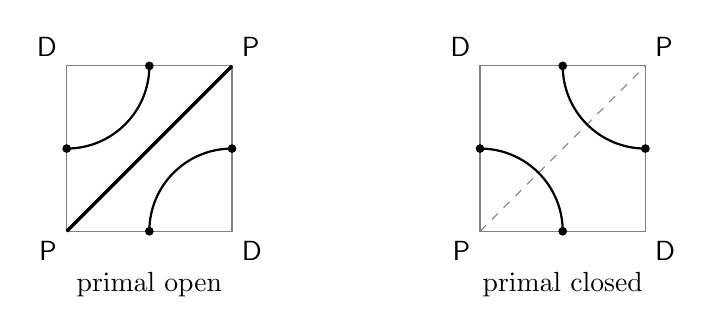
\begin{tikzpicture}[scale=1.05]
 \begin{scope}
  \draw[gray] (0,0) rectangle (2,2);
  \draw[very thick] (0,0)--(2,2);
  \draw[thick] (0,1) arc[start angle=-90,end angle=0,radius=1];
  \draw[thick] (1,0) arc[start angle=180,end angle=90,radius=1];
  \node[below left] at (0,0) {$\mathsf P$};
  \node[above right] at (2,2) {$\mathsf P$};
  \node[above left] at (0,2) {$\mathsf D$};
  \node[below right] at (2,0) {$\mathsf D$};
  \foreach \x/\y in {0/1,1/0,2/1,1/2}
    \fill (\x,\y) circle (1.5pt);
  \node at (1,-.65) {primal open};
 \end{scope}
 \begin{scope}[xshift=5cm]
  \draw[gray] (0,0) rectangle (2,2);
  \draw[dashed,gray] (0,0)--(2,2);
  \draw[thick] (1,0) arc[start angle=0,end angle=90,radius=1];
  \draw[thick] (2,1) arc[start angle=-90,end angle=-180,radius=1];
  \node[below left] at (0,0) {$\mathsf P$};
  \node[above right] at (2,2) {$\mathsf P$};
  \node[above left] at (0,2) {$\mathsf D$};
  \node[below right] at (2,0) {$\mathsf D$};
  \foreach \x/\y in {0/1,1/0,2/1,1/2}
    \fill (\x,\y) circle (1.5pt);
  \node at (1,-.65) {primal closed};
 \end{scope}
\end{tikzpicture}
\caption{The two tile switches. The solid diagonal is an open primal
edge; the dashed diagonal records the absent primal edge. The curved
arcs specify the pairing of ports and hence the order of strand
occurrences when a medial vertex is visited twice.}
\label{prelim:switch-figure}
\end{figure}


For topological arguments, draw the two arcs of a switch disjointly within
its tile, normally to the sides at their ports. This drawing and the straight
medial drawing can be parametrized piece by corresponding piece, preserving
the order of occurrences at a double visit. Their uniform distance is at
most twice the tile diameter. Thus these local changes of drawing disappear
in the curve topology of the theorem.

A wall cuts tile connections at ports. Distinct sectors at a wall corner
have distinct copies of that corner, as on a surface cut open. The end of a
finite slit has one sector of angle $2\pi$. All shapes in the tile arguments
are unions of whole tiles; separating repeated boundary incidences by a
small thickening leaves their combinatorics unchanged.

Partition each boundary component into intervals of alternating designated
wire colors. Within an interval, pair the two intervening ports between
successive occurrences of the designated color, including eligible end
vertices. These are the \emph{local caps}. A genuine change leaves one
unmatched port, on the side whose color differs from the change vertex.
Use the analogous cyclic caps on a boundary component without changes.
Intervals will always be much longer than one mesh.

A \emph{positive cap completion} joins the unmatched ports around the primal
intervals in the added boundary disk. Equivalently, wire each primal
interval separately, with a dual sea between these wires. This adds only
boundedly many connections beyond the local caps when the number of changes
is bounded. It adds no primal identification on a dual interval.

\begin{lemma}[The positive loop law]\label{prelim:loop-law}
On a genus-zero tile surface with positive cap completions, the switch
weight $d^\ell$, where $\ell$ counts completed medial loops, is proportional
to the critical FK weight with the corresponding boundary partition.
Conditional laws on common subdomains are therefore FK laws with induced
partitions. The same assertion holds after interchanging the colors.
On a torus without caps the two weights differ by a factor bounded in terms
of $q$ alone.
\end{lemma}

\begin{proof}
Draw noncrossing exterior primal trees realizing the designated
identifications and thicken the resulting open primal graph. Its perimeter
is the medial loop collection, apart from a fixed number of exterior
components. Euler's formula gives the configuration-dependent part of the
perimeter count as
\[
 \ell=2k_\xi(A)+|A|+\text{constant}.
\]
Since $d^2=q$ and $p_q/(1-p_q)=d$, the weights agree up to a constant
independent of $A$. The domain Markov property gives the conditional-law
statement. On a torus the thickened graph has Euler characteristic
$|V|-|A|=2k-\ell-2g$, with $g\le1$, so the additional factor is bounded.
\end{proof}
\subsection{Crossing estimates and finite plane loops}

We use two distinct crossing inputs. The buffered bulk box-crossing theorem
for canonical weights on doubly periodic isoradial graphs applies for
$1\le q\le4$ \citep[Theorem~1.1]{DCLM2019Isoradial}. Square rhombi have
canonical odds $\sqrt q$, so this includes our square lattice. For example,
for fixed $a>0$, horizontal crossing of
$[-an,an]\times[-n,n]$ inside
$[-(a+1)n,(a+1)n]\times[-2n,2n]$ has probability bounded away from zero
and one, uniformly in the boundary partition on the larger rectangle.
The same theorem gives equality of the free and wired infinite-volume
laws. Hence planar duality at these self-dual odds preserves the plane
loop law, including when a tile translation exchanges the two colors.

When a crossing must reach a domain wall, we use the stronger theorem for
critical square FK with $1\le q<4$: a discrete simple-polygon quad of
bounded continuum extremal distance has an actual open crossing with
probability bounded away from zero, uniformly in its boundary partition
\citep[Theorem~1.2]{DMT2021Fractal}. We do not apply this statement at $q=4$.
FKG and the domain Markov property apply because $q\ge1$; duality supplies
the corresponding statements for the other color.

Here is the concrete wall application needed below. A tile-coordinate
rectangle contains a nearest-neighbor quad of either color graph with
staircase sides within boundedly many mesh layers of its boundary.
The continuum extremal distance required by the theorem is bounded for
bounded aspect ratio. Indeed, straight segments parallel to the crossing
direction join the staircase electrodes through a transverse band whose
width is comparable to the rectangle's width. Their lengths are at most
a constant times its length. Integrating their metric lengths across
this band and applying Cauchy--Schwarz bounds the extremal distance by
the same aspect-ratio constant. The discrete resistance is also bounded:
distribute a unit flow among disjoint zigzag paths whose number is
comparable to the width in mesh units and whose lengths are bounded by
a constant times the length in mesh units. At an electrode on a wall,
the last crossing vertex can
be connected to a wall vertex of the same color using boundedly many fresh
edges. Conditional finite energy bounds the extra cost below uniformly.
Keep the electrode away from the ends of its designated wall interval.

Crossings in a buffered piecewise rectangular corridor follow by using
strips of width a fixed fraction of its clearance and overlapping end
squares. Transversal crossings in these squares join successive
longitudinal crossings; FKG combines the finitely many requirements of one
color. This constructs wall-to-wall paths in annular sectors with openings
$\pi/2,\pi,3\pi/2,2\pi$, including between the two banks of a slit, as
well as circuits in a full annulus. Different colors in tile-disjoint
sectors can be imposed successively by their conditional lower bounds.
All paths here are actual paths. Radii may use tile sup-norm rims, and all
buffers have fixed relative width and sufficiently large fixed mesh width.

\begin{lemma}[Finiteness in the plane]\label{prelim:finite-loops}
For every fixed $1\le q<4$, all medial strands of the specified free
infinite-volume square FK law are almost surely finite loops.
Finite deterministic surgeries admit positive normalized loop laws with
the FK conditional laws of Lemma~\ref{prelim:loop-law}.
\end{lemma}

\begin{proof}
Buffered bulk crossing gives a conditional probability bounded below for
an actual primal circuit around any fixed box in each of successively
separated annuli. The probability of missing the first $m$ such screens
is at most $(1-c)^m$, regardless of the exterior partition. The same
argument gives arbitrarily large actual dual circuits. These two colors
of screens prevent a medial strand meeting the box from escaping to
infinity. Taking the countable union over boxes proves finiteness.

A surgery at finitely many tile connections changes only finitely many
loops at a fixed mesh. Relative to the unmodified plane law, its weight
ratio is $d^{\Delta\ell}$, bounded above and below by constants that may
depend on this finite set of connections. Normalization defines its
positive law. Equivalently, exhaust by planar domains; the same circuit
argument makes the local completion independent of remote boundaries.
Lemma~\ref{prelim:loop-law} then gives the conditional law.
\end{proof}

\subsection{Comparison through a collar}

\begin{lemma}[Bounded densities across a collar]\label{prelim:collar}
Suppose two positive laws have the same graph in a collar between radii
$r$ and $16r$. In this collar the graph is a full annulus, or a bounded
number of sectors separated by straight coordinate walls; coincident slit
banks are allowed. Their deterministic wire portions agree there. Only
boundedly many wire blocks traverse the collar, and no other
identifications jump it. One radial side faces an arbitrary unknown
partition, whereas the graph and deterministic wires toward the other
side are fixed. The marginal densities on edges beyond that other side
are mutually bounded by a constant independent of scale and of the far
graph. Equivalently, their expectations of every nonnegative remote
function are comparable with this same constant.

The conclusion also holds for a fixed-shape rectangular bulk collar
shielding a long box, with a constant depending on its shape.
\end{lemma}

\begin{proof}
First work on a finite graph and a finite remote edge set. Split each
through wire transversally, preserving its connections on each side and
retaining just one representative connection across the cut. The unknown
data induce a partition $\xi$ at their section. Include all common
deterministic wires for every choice of $\xi$.

For two ordered partitions, the likelihood ratio of the coarser law to
the finer law is increasing: the rank of the additional identifications
decreases as open components merge. Write $R$ for this full likelihood
ratio. Its marginal ratio on a remote edge set $E_0$ is
\[
 \mathbb E_{\rm fine}[R\mid\omega|_{E_0}].
\]
Opening remote edges increases both $R$ and the conditional FK law on
the other edges, by partition monotonicity. Thus this marginal ratio is
increasing as well. Consequently its maximum is attained at the all-open
configuration and its minimum at the all-closed configuration. It is
enough to compare those two events for the maximal and minimal partitions;
every other partition lies between them.

An actual primal crosscut in every sector, or a primal circuit in the
annulus, screens the remote graph with uniformly positive probability.
Such screens can be discovered from the unknown side without examining
edges strictly beyond them. In a sector, explore all actual dual paths
from its unknown-facing arc and query edges incident to the reached dual
vertices. If a primal wall-to-wall crossing exists, the search does not
reach the remote arc. The elementary complementary crossing alternative
then places a blocking primal path among the queried edges: otherwise,
setting the unqueried primal edges closed would produce a dual crossing.
The alternative follows by tracing the perimeter of the actual component
reachable from the starting side; corner gap vertices belong to the arcs
when their color permits. The annular version is the alternative between
a primal circuit and a radial dual connection. Perform the searches in a
subcollar leaving space before both sections. Reversing colors gives the
dual searches as well.

Condition on a successful primal search under the minimal law. Each
screen is already connected. Joining all screens and the bounded number
of through-wire representatives requires only boundedly many additional
block identifications. Each has an unnormalized weight ratio in
$[q^{-1},1]$, hence changes expectations by a bounded density factor.
The resulting partition dominates every partition transmitted from the
unknown side. In particular it dominates the maximal law restricted at
this same screen geometry, without requiring that law to contain the
screen. The positive probability of the search proves the desired
comparison of all-open probabilities.

For all-closed probabilities, make the actual dual searches under the
maximal law. No actual primal path crosses these screens. Only the
boundedly many through-wire representatives can still transmit ties;
remove these ties at bounded cost. The resulting free cut is
stochastically smaller on the remote graph than any other imposed cut
partition, including the restriction of the minimal law. This proves
the decreasing-event comparison. The extremal likelihood-ratio argument
now gives the assertion for every remote event and every nonnegative
remote function. Exhaustion proves the infinite-exterior version.
For a rectangular bulk collar use the corresponding enclosing-circuit
searches.
\end{proof}

\begin{lemma}[Relative comparison]\label{prelim:relative-collar}
Under the hypotheses of Lemma~\ref{prelim:collar}, suppose successive
collars have one of the following geometries:
\begin{enumerate}[label=(\roman*)]
\item a full annulus, or one sector whose through wires are precisely
continuous primal wire portions along its side rays;
\item two sectors, with primal wires along both side rays of one sector
and no through wires in the other, and no further fixed contacts
between the sectors.
\end{enumerate}
After $m$ further collars of a sufficiently large fixed radius ratio,
the remote expectations of every fixed nonnegative function under two
possible unknown-side laws have ratio
$1+O((1-c)^m)$, or both expectations vanish. The conclusion holds in
either radial direction, also after positive modifications or tilts
supported on the unknown side.
\end{lemma}

\begin{proof}
Use a radius ratio such as $256$ to leave two subcollars of the preceding
type. Lemma~\ref{prelim:collar}, applied nearer the unknown side, gives a
common marginal part of uniformly positive mass on the other subcollar.
Couple those configurations identically on a fixed fraction of a
reference marginal. In case~(i), additionally impose a primal screen
meeting and joining every through wire. In case~(ii), impose a primal
screen on the wired side and a dual screen on the other side. These
requirements have uniformly positive conditional probability. On their
occurrence the partition transmitted to the next section depends only
on the shared configuration: every route through the unknown region
must enter and leave through a primal screen already connected to its
through wires, and the other sector transmits no primal connection.

For a nonnegative remote function, take the largest and smallest
expectations over partitions at each successive section. Conditioning
nests these intervals of possible expectations. The common part just
constructed contracts their difference by a factor $1-c$. Their ratio
is bounded initially by Lemma~\ref{prelim:collar}; iterating therefore
gives the stated relative estimate. A positive unknown-side tilt is a
mixture over the same partitions. In particular, when propagating away
from a gap, wire connections made or lost inside that gap belong to the
unknown partition, which explains the need for both colors of screen
in case~(ii).
\end{proof}

\subsection{Passages and positive local tilts}

Raw strands use only tile switches and stop when they reach a wall port.
A passage count in a buffered annulus counts disjoint strand passages
through its prescribed inner and outer rims; the outer buffer allows
cropping at both rims.

\begin{lemma}[Exponential passage moments]\label{prelim:passages}
In any fixed buffered annulus or sector of the preceding types, a raw
passage count $X$ satisfies
\begin{equation}\label{prelim:passage-moment}
 \mathbb E[\exp(BX)\mid\text{exterior}]\le C_B
 \qquad(0\le B<\infty),
\end{equation}
uniformly in scale and in exterior states inducing the specified graph
and arbitrary boundary partition. The same holds for a fixed finite
family of macroscopic passage counts in a fixed geometry.
\end{lemma}

\begin{proof}
First obtain one positive exponential rate. Disjoint simple radial
strand subarcs split a slightly cropped annulus into ordered strips.
Along each passage is an actual primal crossing path. Paths in distinct
strips cannot join in the cropped graph, because open primal edges cannot
cross the intervening medial separators. Choose the endpoint rim bands
strictly inside the region traversed by the separators. Thus $X$ passages
force at least $X/2-O(1)$ different crossing components in the actual
cropped graph.

Explore complete actual components successively from one rim, ignoring
all external identifications when deciding membership in a component.
After a component is removed, its incident unexplored boundary edges
are closed. The surviving FK law is dominated by full wiring at the
original rims and walls; removing vertices can only decrease actual
crossings. Even with this full wiring an actual dual blocker across the
cropped annulus has probability at least $c>0$. Conditional on every
successful discovery, the chance of another crossing is therefore at
most $1-c$. The number of components has a geometric tail, proving
\eqref{prelim:passage-moment} for one $B>0$.

To obtain any fixed rate, divide the radial distance into $J$ separated
slices of thickness comparable to $r/J$. Cover a middle rim in each slice
by $O(J)$ small boxes whose buffered annuli remain within the slice.
Use wall-centered boxes near a straight wall and smaller bulk boxes
elsewhere, counting the two sides of a wall separately. The overlap graph
has a bounded coloring independent of $J$. Every original passage crosses
one small annulus in each slice, so
\[
 JX\le\sum_i X_i,
\]
with $O(J^2)$ counts having the first exponential bound. Conditional
iteration within each color class, followed by H\"older across the
bounded number of colors, gives a rate $c'J$. Here iteration uses the
same bound conditional on every configuration outside each buffer;
it does not require independence between buffers. Choose $J$ arbitrarily
large but fixed. Before these boxes fit in the mesh, a deterministic
finite-size bound suffices. A finite covering by bulk, straight-wall,
and corner buffers gives the macroscopic version: a strand segment of
the designated diameter must leave one box of an inner cover whose
outer buffer is much smaller than that diameter.
\end{proof}

Let $N_j$ count raw nests wholly inside radius $r_j$, where the radii are
dyadic and the local sector geometry extends beyond the largest radius
by a buffer. A nest is a closed loop surrounding a bulk site, or an arc
joining the opposite side rays around a boundary gap, corner, change, or
slit tip. Then
\begin{equation}\label{prelim:nest-increments}
 0\le N_j-N_{j-1}\le X_j,
\end{equation}
where $X_j$ is a finite family of passage counts in a band near $r_j$.
Its buffer is disjoint from $B_{r_{j-k}}$ for a fixed $k$. Indeed a newly
included nest either travels a fixed fraction of the radius or goes
around the point within the band. At a slit tip, reaching the other bank
without approaching the tip requires traversing the full-angle sector.
Small-box coverings away from the center give the asserted $X_j$.
Start the levels at a fixed mesh radius so the initial count is bounded.

\begin{lemma}[Local tilt bounds]\label{prelim:tilts}
For fixed $b>0$, put
\[
 F_j=\mathbb E b^{N_j},\qquad
 d\nu_j=F_j^{-1}b^{N_j}\,d\mathbb P.
\]
The ratios $F_j/F_{j-1}$ are bounded above and below uniformly.
Under $\nu_j$, the shell counts $X_i$ at and beyond the outer tilt
level, $i\ge j$, have all fixed exponential moments uniformly bounded.
The assertions remain conditional on exterior data of the specified
geometry and allow adjoining a fixed family of passage counts with
buffers at or beyond that level.
\end{lemma}

\begin{proof}
The case $b=1$ is Lemma~\ref{prelim:passages}. For $0<b<1$, set
$D_i=\log(F_{i-1}/F_i)\ge0$. Jensen's inequality and the exponential
bound give, for any sufficiently small fixed $\varepsilon>0$,
\begin{align*}
 D_i
 &\le |\log b|\,\mathbb E_{\nu_{i-1}}X_i\\
 &\le\varepsilon\log
       \mathbb E_{\nu_{i-1}}
          \exp\bigl(|\log b|X_i/\varepsilon\bigr)\\
 &\le C_\varepsilon+
       \varepsilon\sum_{i-k<l<i}D_l.
\end{align*}
In the last inequality, drop decreasing factors back to level $i-k$.
The remaining tilt is supported outside the buffer of $X_i$, so the
conditional passage bound applies. Choose $\varepsilon(k-1)<1$;
induction bounds every $D_i$. Dropping the same bounded number of levels
then proves every asserted exponential moment.

For $b>1$, choose $B>k\log b$ as large as desired and induct on $j$ that
$\mathbb E_{\nu_j}e^{BX_i}\le C_*$ for $i\ge j$. When $i\ge j+k$,
the tilt and the buffer are disjoint. Otherwise let $j_0=i-k<j$.
The normalizing increment from $j_0$ to $j$ is at least one, so
\[
 \mathbb E_{\nu_j}e^{BX_i}
 \le\mathbb E_{\nu_{j_0}}
 \exp\left(BX_i+(\log b)\sum_{j_0<l\le j}X_l\right).
\]
Give each summand in the sum H\"older weight $\log b/B$ and use the
inductive bound at the earlier tilt $j_0$. The remaining H\"older
factor is an exponential moment of $X_i$ at a larger fixed rate,
whose buffer is disjoint from the tilt at $j_0$. The right side is at
most $C C_*^{k\log b/B}$, which closes the induction for sufficiently
large $C_*$. Negative levels mean no tilt. The moment bounds give the
ratio bounds using \eqref{prelim:nest-increments}. The argument is
unchanged after adjoining the indicated passage counts.
\end{proof}

Consequently the expectations of these local weights and their fixed
powers have logarithms of size $O(\log n)$ up to radius $O(n^C)$ in mesh
units. Changing a cutoff
radius by a fixed factor costs a bounded ratio. Spatially separated local
tilts can be treated successively by conditioning on their disjoint
patches, or by Lemma~\ref{prelim:collar}. Finally, log convexity between
a given power and twice that power shows that increasing the power by
$\varepsilon$ costs only $n^{O(\varepsilon)}$.

\begin{lemma}[Absorbing macroscopic errors]\label{prelim:absorb}
Suppose $Y_n\ge0$, $\mathbb E Y_n\ge n^{-A}/C$, and
$\mathbb E Y_n^2\le Cn^A$, whereas $X_n\ge0$ has uniformly bounded
exponential moments at every fixed rate. For fixed $C_0\ge1$ and every
$\varepsilon>0$,
\[
 C_\varepsilon^{-1}n^{-\varepsilon}
 \le
 \frac{\mathbb E[Y_n C_0^{\pm X_n}]}{\mathbb E Y_n}
 \le C_\varepsilon n^{\varepsilon}.
\]
\end{lemma}

\begin{proof}
Choose $\eta>0$ so that $\eta\log C_0<\varepsilon$ and split at
$X_n=\eta\log n$. On the first event the multiplicative factor lies
between $n^{-\varepsilon}$ and $n^{\varepsilon}$. Cauchy--Schwarz
and the exponential moment bound at an arbitrarily large fixed rate make
both $\mathbb E[Y_n;X_n>\eta\log n]$ and
$\mathbb E[Y_n C_0^{X_n};X_n>\eta\log n]$ smaller than any prescribed
inverse power after accounting for the polynomial second moment.
Choose that power larger than $A+1$. Division by the stated lower bound
for $\mathbb E Y_n$ proves both estimates, enlarging constants for
bounded $n$.
\end{proof}

\subsection{Comparing slit partition functions}

\begin{lemma}[Surface partition comparison]\label{prelim:surface}
Let finitely many straight finite wall segments have fixed macroscopic
shapes and positive mutual separation. Complete each as a positive
isolated boundary slit. Let $Z_s$ be its partition function relative to
the unmodified plane law, and $Z_{\rm all}$ the corresponding partition
function with all slits. Uniformly in the mesh,
\begin{equation}\label{prelim:surface-factorization}
 Z_{\rm all}\asymp\prod_s Z_s.
\end{equation}
Reversing every cap-wire polarity on both banks of a straight isolated
segment with boundedly many changes alters $Z_s$ by a bounded factor.
The same comparison holds for a segment and its image, with transported
cap data, under a symmetry of the homogeneous tile lattice, with the two
color names exchanged when the symmetry exchanges the color lattices.
\end{lemma}

\begin{proof}
Enclose each segment in its own patch with a vacant bulk tile collar and
room for a further disjoint buffer. Let $X_s$ be a passage count through
that collar. Compare the incremental loop change $\Delta\ell_s$ of
the slit surgery with $\Delta\ell_s^\circ$ computed after closing the
patch ports by the same arbitrary pairing before and after the surgery.
Their difference is $O(X_s)$. To see this, cut the segment ports. The
background pairing is determined within the patch except for ends whose
strand first traverses the collar. There are $O(X_s)$ such ends, and
changing their pairing changes either completed cycle count by at most
their number, also when other surgeries have been made outside.

Put $G_s=d^{\Delta\ell_s^\circ}\mathbf1_{\{X_s\le K\}}$.
For fixed sufficiently large $K$, simultaneous truncation has probability
bounded below under the normalized law with all completed slits, by
Lemma~\ref{prelim:passages}. On the truncated event the surgery weights
and their local versions are comparable. Therefore
\[
 Z_{\rm all}\asymp\mathbb E_0\prod_sG_s,
 \qquad Z_s\asymp\mathbb E_0G_s,
\]
where $\mathbb E_0$ is the unmodified plane expectation. Apply
Lemma~\ref{prelim:collar} successively to the separated patch factors
to obtain \eqref{prelim:surface-factorization}.

Translate an isolated segment by one tile step in its tangent direction.
This is a symmetry of the homogeneous plane loop law, with duality
interchanging the colors when needed. Its shifted local caps agree with
the reversed caps except at boundedly many ports near tips and changes.
Their remaining pairings differ on only boundedly many ends, which has
bounded cycle-count cost. Applying such a lattice symmetry to the isolated
slit and its cap data gives the last assertion.
This is a comparison of partition functions; it does not assert bounded
pointwise density for changing all pairings along a wall.
\end{proof}

\section{Logarithmic short-distance comparisons}\label{sec:exponents}

Only the strict range $1\le q<4$ is considered in this section. We require
inequalities between logarithmic costs, not the existence of limiting
critical exponents. Put
\begin{equation}\label{exp:parameters}
 \Delta=\frac{\pi}{2\lambda}-\frac32,\qquad
 s=\Delta+1,\qquad t=-\Delta,\qquad
 f(g)=\frac{\sin((2-g)\lambda)\sin((1+g)\lambda)}
                 {\sin(2\lambda)\sin\lambda}.
\end{equation}
In the local experiments below, the cutoff radius is comparable to $n$
in mesh units, the specified local geometry extends beyond it by a fixed
buffer, and the exterior has any fixed compatible positive completion.

\subsection{Local costs and their conventions}

At a flat change of wire color, let $P(n)$ be the logarithm of the
probability of an actual arm of the gap vertex's color reaching the
cutoff radius. Let $N$ count raw arcs straddling the change, from one
side ray to the other, wholly inside that radius, and set
\[
 D_*(n)=\log\mathbb E[d^N].
\]
At a corner without a wire flip, write $i=0$ if the gap color agrees
with the designated wire color and $i=1$ otherwise. For a convex
right-angle corner and a reentrant right-angle turn respectively, define
\[
 C_i(n)=\log\mathbb E[f(1/2)^{N/2}],\qquad
 L_i(n)=\log\mathbb E[f(-1/2)^{N/2}],
\]
where again $N$ counts local straddling raw arcs. Finally, at a bulk
vertex, let $N$ count closed raw nests surrounding it and set
\begin{equation}\label{exp:bulk-weights}
 F_\pm(a;n)=\mathbb E[u_\pm(a)^N],\qquad
 u_\pm(a)=\frac{\cos((1\pm a)\lambda)}{\cos\lambda},
\end{equation}
for fixed
\begin{equation}\label{exp:charge-range}
 0<a<1,\qquad (1+a)\lambda<\pi/2.
\end{equation}
We usually suppress $n$. In particular,
$D_*\ge0$, $C_i\ge0$, and $L_i\le0$: comparing the products of
sines at their common mean gives $f(1/2)>1$ and
$0<f(-1/2)<1$.

\begin{lemma}[Local conventions and strict arm decay]\label{exp:local-costs}
Changing a cutoff radius by a fixed factor, changing the fixed compatible
exterior completion, applying a tile-lattice symmetry to the experiment, or
interchanging both color names and wire designations changes each of
these logarithms by $O(1)$. The expectations of the local weights,
their fixed powers, and the same arm indicator have logarithms of size
$O(\log n)$. For some $c>0$,
\begin{equation}\label{exp:strict-arm}
 P(n)\le-c\log n+O(1).
\end{equation}
\end{lemma}

\begin{proof}
For nest weights these claims, apart from the signs already noted, are
Lemmas~\ref{prelim:collar} and~\ref{prelim:tilts}. Symmetries of the
local loop weights and caps give the geometric and color symmetries.
At a flat change reflection exchanges the two assignments relative to
the gap color. Bending or erasing distant cap connections changes only
the possible exterior partition.

We give the arm argument because it concerns actual connectivity. In a
tile half-box, boundary regions separated by raw boundary-to-boundary
arcs are precisely the actual color components touching boundary gaps.
Closed interior loops cannot split these boundary classes. If the region
at the marked gap does not reach the outer rim, some raw arc with both
ends on the flat wall straddles the gap. One way to see this is to form
the tree of regions separated by the disjoint arcs. The wall and rim
walks both traverse the tree path between their common end regions.
A wall visit to a region absent from the rim excursion is entered and
left across the same separating edge within the wall portion. Conversely,
a straddling arc cuts off the gap and its actual color paths. Thus absence
of all straddling arcs inside radius $r$ forces an arm to a comparable
radius, and an arm to a larger fixed multiple excludes all such arcs.

Arm probabilities at constant multiples of a radius are comparable.
Given the shorter arm, impose a same-color wall-to-wall screen in an
intermediate annulus and a crossing from its inner side to the desired
outer radius. The arm meets the screen and the added crossing meets it;
FKG and the wall crossing estimates give a uniform extension cost.
The construction is valid under arbitrary distant boundary data.
Starting from a bounded-mesh event and iterating gives a polynomial
lower bound. Conversely, actual opposite-color screens in separated
annuli obstruct the arm and have uniformly positive conditional
probability. Their iteration gives \eqref{exp:strict-arm}. Dual-color
requirements use FKG for decreasing primal events. No wire identification
has been used as an edge of an arm.
\end{proof}

For clarity, a one-sided error denoted $o(\log n)$ in an upper bound
means an allowance
\begin{equation}\label{exp:error-convention}
 \varepsilon\log n+O_\varepsilon(1)
 \quad\text{for every fixed }\varepsilon>0.
\end{equation}
Its constants may depend on all fixed charges and geometric choices.

\begin{proposition}[Three logarithmic comparisons]\label{exp:comparisons}
With the definitions above,
\begin{align}
 2P+2D_*+4(C_0+C_1)&\le o(\log n),\label{exp:rectangle-budget}\\
 C_0+C_1+L_0+L_1&\le o(\log n),\label{exp:corner-budget}\\
 P+\sum_j\log\frac{F_-(a_j)}{F_+(a_j)}
   &\le o(\log n),\label{exp:charge-budget}
\end{align}
where the finite list of fixed charges in the last inequality satisfies
\eqref{exp:charge-range} and $\sum_j a_j=1$.
\end{proposition}

We prove the proposition in three finite auxiliary geometries. Their
common algebra and cap bookkeeping are recorded first. The rectangle
compares the flat-change and convex-corner costs; the long cylinder
pairs convex with concave corners; the charged cylinder compares the
bulk endpoint weights. Reversing all wire designations in each geometry
cancels the positive partition-function ratios between its two winding
expansions.

\subsection{The two winding expansions}

Orient every switch strand and, for either global sign, assign the turn
weight $\exp(\pm i\rho W/2)$, where $W$ is its signed turn. Give both
switches the common coefficient $\sin(\lambda/2)/\sin\lambda$ and sum
consistent orientations. The resulting real arrow tensor is identical
for the two signs. Indeed it requires two incoming arrows. For adjacent
incoming positions only one pairing works and its two turns cancel;
for opposite positions the two pairing contributions sum to
$2\cos(\lambda/2)$. Thus every finite contraction, with any prescribed
boundary spin factors and inserted edge matrices, has the same value
in these two expansions. Common tile coefficients will always cancel.

Traverse a boundary with the domain on its left. Let $\theta_j$ be a
lift of its inward normal angle at port $j$, continued by the boundary
turn at a corner. For spin $c=+1$ or $-1$ according as the arrow points
inward or outward, use
\begin{equation}\label{exp:boundary-spin}
 b_j(c)=(2\sin\lambda)^{-1/2}
          \exp\{ic(\rho\theta_j/2+\lambda h_j)\}.
\end{equation}
A raw arc from port $i$ to port $j$ bounding a disk against the
intervening forward boundary interval has turn
$\theta_j-\theta_i-\pi$: close it against that interval, using the
normal endpoint tangents. Summing its two orientations cancels curvature
in the positive-sign expansion and gives
\begin{equation}\label{exp:arc-weight}
 w(h_i-h_j),\qquad
 w(m)=\frac{\cos((m-1/2)\lambda)}{\sin\lambda}.
\end{equation}
For the negative-sign expansion set $h'_j=-h_j-\theta_j/\pi$;
its weight is $w(h'_i-h'_j)$.

Take $h_j=H_j+\Delta\mathbf1_{\{j\text{ high}\}}$, where $H$ is
piecewise constant. A port is high if its immediately preceding gap
vertex in the interval has the designated wire color. Across a wire
flip the adjacent ports are both high or both low. Since the ports
strictly inside a disk arc's boundary interval pair among themselves,
its endpoint high statuses are opposite for an even number of flips
and equal for an odd number. Thus
$h_i-h_j$ is the sum of the drops of $H$ plus $r\Delta$, where
$r=\pm1$ for an even number of flips (positive when the first port is
high) and $r=0$ otherwise. In the negative-sign expansion, high ports
refer to the complementary wires; base drops are negated and augmented
by the boundary turn divided by $\pi$. The identities
\begin{equation}\label{exp:staggered-weights}
 w(g+\Delta)=\frac{\sin((2-g)\lambda)}{\sin\lambda},
 \qquad
 w(g-\Delta)=\frac{\sin((1+g)\lambda)}{\sin\lambda}
\end{equation}
give weights $d,1$ at zero drop.

\begin{lemma}[Local cap elimination]\label{exp:cap-elimination}
For disk arcs whose boundary intervals contain at most one wire flip,
their positive cap-loop factors are $d$ for a zero-flip high starting
port and $1$ for a zero-flip low starting port or a one-flip arc, up to
a bounded overall loop-count error and an error $d^{O(X)}$ for remaining
macroscopic arcs. A nest of $N$ straddling arcs at a corner of turn
$g\pi$ without a wire flip has negative-expansion weight relative to
its caps comparable to $f(g)^{N/2}$.
\end{lemma}

\begin{proof}
Take a family of disk arcs closed under the arcs inside their disks,
with no holes, and remove them from the inside outward. Removing two
adjacent remaining endpoints creates a loop exactly when their exterior
partners already pair them; otherwise reconnect those partners.
The caps still pair successive high-low ports on each remaining
interval, with arbitrary pairings of its unmatched ends. A high-low arc
within an interval creates one loop. A low-high arc merely transports
the pattern. Across a flip, equal high statuses transport an unmatched
end without creating a loop. If two transported unmatched ends were
already tied, the extra loop erases an entire remaining interval. There
are boundedly many such exceptions; also allow the final bounded error
for a no-flip circle. The unremoved boundary loops are at most the number
of remaining arcs.

Include all sufficiently small arcs, together with arcs inside their
disks. Any others contribute a macroscopic passage count $X$ in boundary
bands. Along a local straddling nest the starting parities alternate,
because ports between consecutive starts pair internally on that side.
The two relative weights in \eqref{exp:staggered-weights} multiply to
$f(g)$ after division by the corresponding cap weights $d$ and $1$.
One unpaired factor is bounded. This proves the claimed $f(g)^{N/2}$
comparison. Cutoff patches are disjoint with wider buffers, and a
straddling arc omitted because it exits its patch is charged to $X$.
\end{proof}

\subsection{A rectangle: the flat-change and convex-corner costs}

\begin{proof}[Proof of \eqref{exp:rectangle-budget}]
Take a convex tile rectangle with both side lengths comparable to $n$.
Put a change in the middle of the bottom side and another in the middle
of the top side. Give $H$ drops $s,t$ at these changes and no others.
Since $s+t=1$ and the total boundary turn is $2\pi$, the factors
\eqref{exp:boundary-spin} are periodic around the contour.

In the positive-sign expansion, an arc not separating the changes uses
an interval containing neither change and has its ordinary cap weight.
An arc enclosing one change has $w(s)=w(t)=1$. Closed interior loops
have weight $d$. Lemma~\ref{exp:cap-elimination} and
Lemma~\ref{prelim:passages} therefore bound the spin partition function
above by a constant times the positive cap partition $Z_+^{\rm cap}$.
The latter includes the common tile coefficients.

In the negative-sign expansion the change drops are $-s,-t$ and each
convex corner contributes $1/2$. An arc containing neither change has
an interval containing at most two corners and has positive weight for
both high statuses. An arc separating the changes can use the interval
containing the $s$ mark and $k$ corners; its weight is
$\sin(k\lambda/2)/\sin\lambda$. These weights are nonnegative and
vanish exactly for $k=0$, namely a straddling arc on the bottom side.
Let $E$ be the event that the $s$-gap vertex has an actual path of its
color to another side of the rectangle. Every weight is strictly
positive on $E$, and the local straddles at $t$ have weight $d$.
Relative to the cap law with the complementary wires, the spin
partition is consequently at least
\begin{equation}\label{exp:rectangle-lower}
 \mathbb E_-
 \left[\mathbf1_E d^{N_t}
    \prod_{v\text{ corner}} f(1/2)^{N_v/2}
    C^{-(1+X)}\right].
\end{equation}
Here $X$ counts macroscopic boundary passages. For instance, choose all
small arcs below a fixed diameter fraction so their disks contain at
most one feature. The cap elimination accounts for those arcs, and
remaining factors on $E$ lie in a fixed finite set of positive values.

Without $C^{-(1+X)}$, the expectation in
\eqref{exp:rectangle-lower} is bounded below by a constant times
\[
 \exp\left(P+D_*+\sum_v C_{i(v)}\right).
\]
Indeed the separated positive local factors compare conditionally by
Lemma~\ref{prelim:collar}. After conditioning on their small patches,
extend the local $s$ arm through a fixed corridor avoiding those patches
to another side, by the screens and crossing extensions in
Lemma~\ref{exp:local-costs}. The remaining law is FK with an induced
partition. Lemma~\ref{prelim:absorb} loses only
$n^\varepsilon$ upon reinstating the passage factor, because all local
first and second moments have polynomial cost by
Lemma~\ref{prelim:tilts}.

Choose odd horizontal tile length and even vertical tile length. The
four corners then have the same relative gap-versus-wire type, since
the left and right sides belong to opposite wire intervals. Compare the
two tensor expansions and repeat on this very same rectangle with every
wire polarity reversed. The ratios
$Z_+^{\rm cap}/Z_-^{\rm cap}$ cancel upon multiplication. One run has
four type-$0$ corners and the other four type-$1$ corners; both have the
same $P,D_*$ up to bounded changes of local convention. Taking logarithms
proves \eqref{exp:rectangle-budget} with the error convention
\eqref{exp:error-convention}.
\end{proof}

\subsection{A long cylinder: balancing the two corner turns}

\begin{proof}[Proof of \eqref{exp:corner-budget}]
Take a tile cylinder whose spatial period has two positive coordinate
components, each comparable to $n$, with even sum. In a lift, its lower
boundary repeats all the east steps followed by all the north steps.
The upper boundary is a parallel translated copy at transverse distance
of order $Kn\log n$, where $K$ will be a sufficiently large fixed
constant. Each boundary has one convex and one concave corner. There
are no wire flips and $H$ is constant. Use positive caps for the
reference laws and free periodic spin contraction, with no flux
projection, for the tensor. The normal-angle lift is periodic.

Every same-boundary raw arc bounds a disk against the boundary interval
it cuts off. Its lifted endpoint interval spans less than one period:
otherwise its endpoints and those of a translate would interleave,
forcing intersecting arcs. Its positive-expansion weights are ordinary
cap weights, and its negative-expansion drops are $0$ or $\pm1/2$,
so those weights are positive. A contractible interior loop has weight
$d$. An essential loop has total turn zero and hence weight $2$; the
zero-turn assertion follows by isotopy of a simple generator in the
flat cylinder.

Reserve bottom and top bands of width $O(n)$ containing all boundary
features and their enlarged buffers. In the empty middle strip let
$k_0$ count essential closed medial loops wholly within that strip, and
put
\begin{equation}\label{exp:middle-tilt}
 M=(2/d)^{k_0}.
\end{equation}
It depends only on middle-strip tiles and is at least one. Under either
positive cap law,
\begin{equation}\label{exp:middle-moments}
 \mathbb E M^p\le n^{O_p(K)}\qquad(p<\infty).
\end{equation}
To prove this, cover the middle strip by $O(K\log n)$ buffered bulk
boxes of size a small fraction of the period. Each essential loop
supplies a passage, and conditional iteration of
Lemma~\ref{prelim:passages} with a bounded coloring proves the bound.
Essential loops omitted from $M$, macroscopic boundary arcs, and other
macroscopic loops approaching features are charged to a count $X$ in
the enlarged boundary bands. This $X$ has all fixed exponential moments
uniformly, independently of $K$.

Let $T$ be the event of a raw arc joining the two boundaries. Then
$M=1$ on $T$, and
\begin{equation}\label{exp:through-rarity}
 \mathbb P_\pm(T)\le C n^{-cK}.
\end{equation}
Indeed, in each successive transverse band of width comparable to the
period, actual crossings can form a noncontractible cycle of one color.
Use a necklace of overlapping strip crossings with transversal joins;
its buffers are injective on the cylinder. In the lift the connected
crossings continue through every translate, and their projection
contains a noncontractible cycle. FKG and crossing estimates give a
uniform conditional success probability. Such a cycle blocks $T$, so
iteration through order $K\log n$ bands proves
\eqref{exp:through-rarity}.

The positive expansion has absolute partition value at most
\[
 Z_+^{\rm cap}\,\mathbb E_+[M C^{1+X}].
\]
Off $T$, the negative expansion is positive and its integrand relative
to $Z_-^{\rm cap}$ is at least
\[
 M\prod_v f(g_v)^{N_v/2}C^{-(1+X)},
 \qquad g_v\in\{1/2,-1/2\}.
\]
On $T$, its absolute integrand is bounded by the same local factors
times $C^{1+X}$, without $M$. These statements are
Lemma~\ref{exp:cap-elimination}; through arcs are macroscopic, so their
bounded weights are included in $X$. H\"older, the polynomial local
tilt bounds, and \eqref{exp:through-rarity} bound the possible signed
through contribution by $n^{-c'K+O(1)}$ relative to its caps.

Condition on the middle-strip tiles and use the separated feature
patches to compare the positive main expectation, without its $X$
factor, to
\[
 (\mathbb E_-M)
 \exp\left(\sum_{v:g_v=1/2}C_{i(v)}+
           \sum_{v:g_v=-1/2}L_{i(v)}\right).
\]
It is bounded below by an inverse power of $n$ whose exponent is
independent of $K$, because $M\ge1$. Choose $K$ large enough that the
through error is negligible. Now keep $K$ fixed and apply
Lemma~\ref{prelim:absorb}, using \eqref{exp:middle-moments}, to absorb
all $C^{\pm X}$ factors at an arbitrarily small power loss.

Choose the two boundary wire colors and run the comparison, then
repeat with both colors reversed on exactly the same cylinder, cutoffs and
middle strip. Tensor equality cancels the two ratios of
$Z_\pm^{\rm cap}\mathbb E_\pm M$ when the inequalities are multiplied.
The two runs together count twice each of $C_0,C_1,L_0,L_1$.
Taking logarithms and dividing by two proves
\eqref{exp:corner-budget}.
\end{proof}

\subsection{A charged cylinder: the bulk costs}

\begin{proof}[Proof of \eqref{exp:charge-budget}]
Use a cylinder with straight horizontal boundaries, with even horizontal
period comparable to $n$, and lower boundary traversed eastward. Put the
two flat changes on the bottom, separated by order $n$, and no change
on top. Place the finitely many bulk points $z_j$ at mutually separated
distances of order $n$ in the bottom band. Their buffered cutoff patches
are disjoint; make the band wide enough to leave clear corridors nearer
the bottom. The height is again of order $Kn\log n$.

Draw tile-edge strings from the $s$-gap to each $z_j$ and multiply the
spin crossing its string by $\exp(-i\lambda a_j c)$, where $c=+1$
denotes an arrow along the left normal of the oriented string step.
Use raw drops $s-1,t$ for $H$ on the lower boundary, with total zero,
and constant $H$ on top. Oriented intersections give the following
sign convention: in the positive expansion, a string of charge $-a_j$
shifts a boundary disk arc's cosine argument, in units of $\lambda$,
by $+a_j$ for a launch in its interval and by $-a_j$ for an endpoint
in its disk. The boundary child lies to the arc's right when the arc
is followed from the earlier to the later port. Thus the local effective
bottom drops are $s,t$; in the negative expansion they are $-s,-t$,
with $a=\sum_{z_j\text{ in disk}}a_j$ added for the endpoints inside.

For a boundary disk arc the negative-expansion numerators, over the
common denominator $\sin\lambda$, are
\begin{equation}\label{exp:charged-table}
\begin{array}{c|l}
 \text{number of enclosed flips}&\text{numerators}\\ \hline
 0&\sin((2-a)\lambda),\quad\sin((1+a)\lambda)\\
 1&\sin(a\lambda)\quad[s],\qquad
      \sin((2-a)\lambda)\quad[t]\\
 2&\sin((3-a)\lambda),\quad\sin(a\lambda).
\end{array}
\end{equation}
The interval spans less than one period, so each change is counted at
most once. Top boundary disks use the zero-flip row. Since $0\le a\le1$
and $0<\lambda\le\pi/3$, every entry is nonnegative. A vanishing
entry always belongs to a child interval containing $s$; this includes
the additional zero $\sin(3\lambda)=0$ at $q=1$ in the two-flip row.
Contractible closed loops in the negative expansion have relative weight
$\cos((1-a)\lambda)/\cos\lambda>0$; their interior is on the left
for counterclockwise orientation. The two expansions therefore give
the prescribed local weights $u_\pm(a_j)$. Essential loops have
positive weight $2\cos(a\lambda)$, where $a$ is the charge separated
from the launches, and loops in the empty middle strip have weight $2$.
Keep $M$ as in \eqref{exp:middle-tilt}.

Let $E$ be the event that the $s$-gap vertex connects by actual paths
of its color to a noncontractible open cycle. Construct that cycle near
the bottom, before the conditioned endpoint patches and middle strip.
Conditionally on those patches and the middle,
\[
 \mathbb P_-(E\mid\text{patches and middle})\gtrsim e^P.
\]
This follows from the local arm comparison, same-color FKG and crossing
extension, and the periodic necklace construction used for
\eqref{exp:through-rarity}. On $E$ no child disk arc can cut off $s$,
since the noncontractible cycle cannot fit behind it, and there is no
through arc.

Set $U_\pm=\prod_j u_\pm(a_j)^{N_j}$ and let $Y_\pm$ be the spin
integrands relative to their respective positive cap laws. Local cap
and loop counting gives
\begin{align*}
 |Y_+|&\le M U_+ C^{1+X},\\
 Y_-&\ge M U_- C^{-(1+X)}\quad\text{on }E,\\
 Y_-&\ge0\quad\text{off }T.
\end{align*}
The local $t$-straddles in the negative expansion contribute $d$ each,
which may be discarded in this lower bound. A loop whose endpoint
enclosure differs from a local nest has a macroscopic passage near a
feature: a contractible disk containing $z_j$ must separate it from
the bottom. Thus it is charged to $X$, with all cutoffs small compared
with the feature separations. On the through event $T$ one still has
\[
 |Y_-|\le U_-d^{N_t}C^{1+X},\qquad M=1.
\]
All these local costs are polynomial and the through probability is
$O(n^{-cK})$, so choose $K$ fixed and large to dominate the signed
through error.

Conditioning and Lemma~\ref{prelim:collar} compare the separated local
factors to $\prod_jF_\pm(a_j)$, the middle factor to
$\mathbb E_\pm M$, and the event $E$ to its lower arm cost $e^P$.
Lemma~\ref{prelim:absorb} removes the passage errors at $n^\varepsilon$
cost. Repeat with every wire designation reversed, using the same
domain, strings, drops, cutoffs and $M$. Equality of the two tensor
expansions cancels both cap and middle-factor ratios upon multiplying
the two comparisons. The resulting inequality is
\[
 2P+2\sum_j\log\frac{F_-(a_j)}{F_+(a_j)}
 \le o(\log n),
\]
which gives \eqref{exp:charge-budget}.
\end{proof}

\subsection{The polygon budget}

We now combine the rectangle and corner comparisons for a polygon with
balanced corner types, retaining a strictly negative contribution from
the arm logarithm $P$.  The final assertion records the separate charge
estimate in the form needed below.

\begin{corollary}[Balanced corner parities]\label{exp:polygon-budget}
Let a fixed simple rectilinear polygon have $m$ concave and $m+4$
convex true corners, with wire changes in side interiors. It has tile
approximants differing by $O(1)$ mesh units such that at least
$\lfloor m/2\rfloor$ corners of each relative wire type occur in each
of the convex and concave sets, also after global wire reversal.
For these approximants,
\begin{equation}\label{exp:polygon-saving}
 3P+D_*+\sum_{v\,\mathrm{convex}}C_{i(v)}
       +\sum_{v\,\mathrm{concave}}L_{i(v)}
 \le\frac12P-\frac32D_*+o(\log n).
\end{equation}
Each fixed family of negative endpoint charges with magnitudes summing
to one has total wrong-to-correct local logarithmic cost at most
$-P+o(\log n)$.
\end{corollary}

\begin{proof}
First prescribe the desired relative corner types for one designation.
There remain at least four spare convex corners, one of which adjusts
the parity of the sum of the absolute corner parities. If $b_i$ denotes
the integer coordinate parity of side $i$, a corner between sides
$i-1$ and $i$ has parity $p_i=b_{i-1}+b_i$ modulo two. This cyclic
system is solvable exactly when $\sum_i p_i=0$ modulo two. Choose the
side coordinates with those parities within boundedly many mesh units
of the prescribed ones. For the fixed simple polygon, sufficiently
small independent shifts preserve simplicity. Global wire reversal
just exchanges the relative types.

Pair the balanced convex and concave sets and apply
\eqref{exp:corner-budget}. If $m$ is even, four convex terms remain;
if $m$ is odd, five convex terms and one nonpositive concave term remain.
Since $C_i\ge0$, Equation~\eqref{exp:rectangle-budget} implies
\[
 P+D_*\le o(\log n),\qquad
 C_i\le-\tfrac12(P+D_*)+o(\log n).
\]
The first inequality permits paying for five convex terms even when
only four remain, at an additional one-sided $o(\log n)$ error.
This yields \eqref{exp:polygon-saving}. The same first inequality is
the corresponding flat budget when there are no corner factors.
The endpoint-charge assertion is exactly
\eqref{exp:charge-budget}.
\end{proof}

\section{Angular transfer and its two leading modes}\label{sec:angular}

Throughout this section, $1\le q<4$, $d=\sqrt q=2\cos\lambda$,
$\rho=\lambda/\pi\in(0,1/3]$, $v=\pi/2$, and $Q=-e^{i\lambda}$.
The argument has two parts. We first construct a Hilbert space from
infinite-plane row correlations and prove an angular estimate there. We
then identify its scalar products with reflection across diagonal cuts
of the physical square array. Boundary conditions enter the resulting
estimate through the norms of the exterior states.

\subsection{Rows, twists, and the estimate}

The local row algebra is the six-vertex form of the planar loop
transfer formalism \citep{TemperleyLieb1971,BaxterKellandWu1976}.
Its finite identities are verified below; the infinite-plane
reflection space and the angular decay estimate require the additional
analytic arguments of this section.

In the spin basis $+,-$, set
\[
 J=\begin{pmatrix}0&1\\1&0\end{pmatrix},\qquad
 L_-=|-\rangle\langle+|,\quad L_+=|+\rangle\langle-|,
 \qquad K(\zeta)=\operatorname{diag}(\zeta,\zeta^{-1}).
\]
Here and below twists satisfy $|\zeta|=1$. In the ordered pair basis
$++,+-,-+,--$, let
\begin{equation}\label{bulk:R}
 R(u)=\begin{pmatrix}
 a(u)&0&0&0\\0&b(u)&1&0\\0&1&b(u)&0\\0&0&0&a(u)
 \end{pmatrix},\qquad
 a(u)=\frac{\sin(\lambda-u)}{\sin\lambda},\quad
 b(u)=\frac{\sin u}{\sin\lambda}.
\end{equation}
Time and space steps have unit length and angles $\alpha_t$ and
$\omega_j$. Their successive sums give a rhombic tile array; initially
$0<\omega_j-\alpha_t<\pi$. A spin is positive when its arrow points
along the left normal of the corresponding step. If $h_0,h_1$ are the
two time sides before and after advancing in space, and $s_0,s_1$ the
two space sides before and after advancing in time, the tile tensor
has output indices $(h_0,s_1)$, input indices $(h_1,s_0)$, and value
$R(\rho(\omega_j-\alpha_t))$.

On a spatial circle of even size $N$, write
\begin{equation}\label{bulk:finite-row}
 T_N^D(\alpha)=\operatorname{Tr}_c
 D_cR_{c0}(\rho(\omega_0-\alpha))\cdots
 R_{c,N-1}(\rho(\omega_{N-1}-\alpha)).
\end{equation}
The auxiliary index is $c$. At the seam, $D_{x,y}$ uses the spin $x$
from tile $-1$ and $y$ from tile $0$. Let $\Omega_N$ be the positive
unit Perron vector of the untwisted rows on the zero-total-spin
sector, and $\Lambda_N(\alpha)$ their eigenvalue. Normalized rows are
$A_N^D(\alpha)=T_N^D(\alpha)/\Lambda_N(\alpha)$.
Their common Perron data, and the limiting operators $A^D(\alpha)$,
are constructed below. In the homogeneous transverse array
$\omega_j=v$, put
\begin{equation}\label{bulk:MN}
 \begin{aligned}
 P_\zeta(z)=A^{K(\zeta)}(z),\qquad
 M(z)&=e^{i\tau\rho z}A^D(z),\\
 N(z)&=M(z)P_\zeta(z)+P_\xi(z)M(z),
 \end{aligned}
\end{equation}
where
\begin{equation}\label{bulk:charges}
 \zeta/\xi=Q^\epsilon,\quad \epsilon\in\{-1,1\},\qquad
 (D,\tau)=(L_-,\epsilon)\ \text{or}\ (L_+,-\epsilon).
\end{equation}
The two summands of $N$ describe the two possible positions of a
source in two consecutive rows of the same angle. Products act from
right to left: rows before the source carry twist $\zeta$, and rows
after it carry twist $\xi$. Thus a source in the second row gives
$MP_\zeta$, whereas one in the first gives $P_\xi M$. The phase in
$M$ records the direction of the source row. Section~\ref{sec:current}
will identify this sum with a two-step path increment; here we prove
the row estimate independently of the path's exterior geometry.

\begin{theorem}[Angular transfer estimate]\label{bulk:angular-estimate}
Fix a compact interval $I\subset(-v,v)$. Let $B_{\rm in}$ be a
product of $P_\zeta$ rows and $B_{\rm out}$ a product of $P_\xi$ rows,
at real angles in $[-v,v]$. Suppose each product contains at least
$n\ge1$ angles in $I$. Uniformly for $x,y\in[-v,v]$,
\begin{align}
 \|B_{\rm out}N(x)B_{\rm in}\|&\le Cn^{-1+\rho},
 \label{bulk:low-estimate}\\
 \|B_{\rm out}\{N(x)-e^{i\tau(x-y)}N(y)\}B_{\rm in}\|
 &\le Cn^{-1-\rho}.\label{bulk:high-estimate}
\end{align}
The constant depends on $q$ and $I$. Boundedly many additional pairs
of before-twist rows may be inserted immediately to the right of
$N$, and additional pairs of after-twist rows immediately to its
left. The two terms in \eqref{bulk:high-estimate} may use different
such insertions; on each side their counts must be even. The
constant may depend on a bound for these counts. Multiplication of
$D$ by a common scalar multiplies the bounds by its absolute value.

The same estimates hold in the physical square array sliced in a
diagonal time direction: its time angles are $\pm\gamma_0$, where
$\gamma_0=\pi/4$, and its space angles alternate between
$\pi-\gamma_0$ and $\gamma_0$. The exterior states may contain any
finite number of physical row and spin insertions outside the
sandwich. A scalar contraction is bounded by the displayed rate
times the two reflection norms, with the squares centered on a cut
included in its reflection kernel.
\end{theorem}

The improvement in the second estimate comes from removing one angular
mode, not from assuming that the exterior states have bounded norms.
We first construct the plane reflection space and continue its rows
analytically in the angle. Boundary unitarity then controls the scalar
spectral functions near modulus one. A product of $n$ strict rows
selects spectral energies of order $n^{-1}$. On those low bands,
endpoint reversal singles out the mode $e^{i\tau x}$ with bound
$O(n^{-1+\rho})$; the next odd mode and the remaining errors have
bound $O(n^{-1-\rho})$.
The combination in \eqref{bulk:high-estimate} cancels the former.
The final subsection transfers this estimate, with its exterior norms,
to diagonal cuts of the physical square array.

\subsection{Row algebra and the infinite-plane state}

The finite-dimensional identities used throughout are
\begin{align}
 R_{12}(x-y)R_{13}(x)R_{23}(y)
 &=R_{23}(y)R_{13}(x)R_{12}(x-y),\label{bulk:YB}\\
 R(u)R(-u)&=(1-b(u)^2)I,\label{bulk:inversion}\\
 J_cR(u)^{t_c}J_c&=R(\lambda-u).\label{bulk:crossing}
\end{align}
For completeness, the nontrivial one-minus block of
\eqref{bulk:YB} is symmetric precisely by the three sine identities
\[
 b(x-y)+a(x)b(y)=b(x)a(y),\qquad
 b(y)+a(x)b(x-y)=b(x)a(x-y),
\]
\[
 a(x)+b(x-y)b(y)=a(x-y)a(y).
\]
Spin reversal gives the one-plus block; the remaining blocks are
scalar. The other identities follow directly from \eqref{bulk:R}.
Sliding the intertwiner in \eqref{bulk:YB} through two complete rows
shows that transfers with a common diagonal twist commute: the
intertwiner preserves total spin and hence commutes with the tensor
square of that twist. For arbitrary insertions $D,E$, the same
operation conjugates $D\otimes E$ by a two-spin intertwiner.
Expanding the conjugated matrix in matrix units expresses the
exchanged rows as a finite sum with new insertions. Its coefficients
are analytic wherever that intertwiner is invertible. Division by
the scalar Perron eigenvalues preserves this exchange identity.

For strict angles, the untwisted transfer is primitive on each
total-spin sector. It has positive diagonal entries; moreover an
auxiliary spin can swap with any chosen opposite pair of site
spins, without swapping at the other sites. Such exchanges connect
the sector. Commutation therefore gives common positive left and
right Perron vectors. In the homogeneous array, auxiliary
transposition reverses the product in \eqref{bulk:finite-row}, since
the distinct site operators commute. Equation \eqref{bulk:crossing}
then gives
\begin{equation}\label{bulk:adjoint}
 A^D(\alpha)^*=A^{J\overline D J}(-\alpha)
 \qquad(\alpha\in\mathbb R).
\end{equation}
The corresponding finite-volume identity makes the left and right
vacua equal.

More explicitly, a formal row word $h$ specifies a finite list
$(D_1,\alpha_1),\ldots,(D_m,\alpha_m)$ of matrices and strict angles.
Its finite-circle vector and vacuum coefficient are
\[
 h_N=A_N^{D_m}(\alpha_m)\cdots A_N^{D_1}(\alpha_1)\Omega_N,
 \qquad \langle\Omega_N,h_N\rangle.
\]
For two such words $h,g$, the proposed Gram form is
\[
 \langle h,g\rangle=\lim_{N\to\infty}\langle h_N,g_N\rangle.
\]
The following lemma establishes these limits. The empty word becomes
$\Omega$, and prefixing a row to the operator product defines its left
action. A bare vacuum coefficient means the same limit with the empty
word in the first slot; the adjoint identity expresses every Gram
coefficient as such a coefficient of a longer word.

\begin{lemma}[Plane kernels]\label{bulk:plane-kernels}
Finite words of homogeneous normalized strict-angle rows have
limiting Gram matrices as $N\to\infty$. Their quotient and completion
give a separable Hilbert space $\mathcal H$ with unit vector $\Omega$
and bounded left row actions satisfying
\begin{equation}\label{bulk:row-bound}
 \|A^D(\alpha)\|\le2\|D\|.
\end{equation}
Bare vacuum coefficients are continuous in strict angles and are
unchanged by a common translation of all time angles, as long as
the translated angles remain in $(-v,v)$.
\end{lemma}

\begin{proof}
We first identify the plane state, including the effect of the
zero-spin projection. Take periodic lists of time and space angles
in a strict range, with the two direction ranges ordered and
transversely separated in a half-circle. Use tori whose period
sizes are even multiples of the list periods. The resulting
rhombic square array is embedded and has bounded angles. Indeed
the cyclic order at each vertex gives local injectivity, while
averages of runs of either family have uniformly positive length
and uniformly transverse directions. Thus index distances control
Euclidean distances in both directions, giving properness and
global embedding.

Expand each $R$ into its two adjacent-side pairings with oriented
turn weight $e^{i\rho W/2}$. The pairing at the corner between the
two positive steps, and at its opposite corner, has coefficient
$a(u)$; the other pairing has coefficient $b(u)$. For example, the
mixed entry follows from
$a(u)e^{iu}+b(u)e^{-i(\lambda-u)}=1$ and its conjugate. In a
single-pairing entry the two turns cancel. A contractible loop
therefore has weight $d$. An essential simple oriented torus loop
has total turn zero. All essential loops are parallel up to
orientation. Their number $k$ is even, by the even intersection
parities with both period cycles and primitivity of their common
homology class. The allowed orientation count after projection
onto zero spin on either chosen quantum section is
\begin{equation}\label{bulk:essential-count}
 \chi=2^k\quad\text{if the intersection is zero},\qquad
 \chi=\binom{k}{k/2}\quad\text{otherwise}.
\end{equation}
Since $d<2$, there is $c(d)>0$ such that
$c(d)d^k\le\chi\le2^k$ for every even $k$.

Replacing $\chi$ by $d^k$ gives the canonical isoradial FK law,
up to the bounded torus genus factor of Lemma
\ref{prelim:loop-law}. To check the parameter, the relative
open weight at a primal corner between the positive steps is
$\sqrt q\,b/a$, and at the other primal corner it is
$\sqrt q\,a/b$. If $\gamma$ is the angle at the primal corner, the
odds divided by $\sqrt q$ are
\[
 \frac{\sin(\rho\gamma)}{\sin(\rho(\pi-\gamma))}.
\]
This is the canonical weight, with the complementary-angle
convention of \cite[Equation~(1.1), Theorem~1.1, and Equation~(1.3)]{DCLM2019Isoradial}. That theorem applies
to these fixed doubly periodic bounded-angle isoradial grids. It
gives uniqueness and buffered crossing estimates, uniformly over
the boundary partition on the outer buffer. The bulk passage-count
argument of Lemma \ref{prelim:passages} consequently applies
on each such grid. No estimate as an angle degenerates is used.

Here is why the essential-orientation tilt does not change the
local limit, even for unbounded aspect ratios. Let $r\le R$ denote
the shorter and longer period sizes. Cover the torus by $O(R/r)$
buffered boxes of size a small fraction of $r$, with a bounded
number of disjoint-buffer colors, so that every essential loop
crosses one of them. Include $O(R/r)$ translates, by medium periods,
of a target annulus about the query. Let $Y$ be the sum of the
passage counts in this cover. For each fixed $c>0$, conditional
passage moments, iteration within each color, and H\"older's
inequality give
\begin{equation}\label{bulk:torus-moment}
 \mathbb E e^{cY}\le e^{C_cR/r},\qquad k\le Y.
\end{equation}
The density of the tilted law is bounded above by $C e^{c_0Y}$
before normalization and its normalizing denominator is bounded
below. Consequently
$\mathbb E_{\rm tilt}e^Y\le C e^{CR/r}$, and Jensen's inequality
gives $\mathbb E_{\rm tilt}Y\le CR/r$. Translation invariance then
bounds the expected count at the target annulus uniformly.

Condition on the exterior of its inner box. The number of exterior
excursions from that boundary to distances comparable to $r$ before
returning is tight. If it is at most $K$, changing the filling
can alter only $O(K)$ essential loops: every affected loop must
leave the injective chart along such an excursion. The common
homology class can change only when no essential loop remains
unaffected. Thus the ratios of the genus and orientation tilt over
all fillings are bounded in terms of $K,q$. For the binomial case
this also follows directly by comparing central binomial
coefficients with indices differing by $O(K)$; a switch between
the two cases in \eqref{bulk:essential-count} can occur only when
there are $O(K)$ essential loops. The conditional inner law is
therefore comparable with FK under the induced partition.
Apply this density comparison once to the whole event that an arm or
medial strand from a fixed window reaches distance comparable to $r$.
On the event of at most $K$ exterior excursions, its conditional
probability is at most $C(K,q)$ times the corresponding FK bound.
Successive buffered circuits make that FK bound tend to zero as
$r\to\infty$. The excursion count is tight, so the complementary
probability becomes arbitrarily small by then letting $K\to\infty$.
No density factor is accumulated separately at each circuit scale.

Now condition outside a large fixed test box containing the query,
and let $z_0$ be its center. Choose a fixed $\eta>0$ so small that the
torus metric ball $B_T(z_0,2\eta r)$ has an injective planar lift;
the transverse period bounds above give this uniform choice. For large
$r$ the fixed box lies in $B_T(z_0,\eta r/2)$. The preceding escape
estimate shows that, with probability tending to one, no exterior
actual component or medial arc incident to the box reaches the rim of
$B_T(z_0,\eta r)$. Every such object is connected and meets the box,
so their entire union, together with every possible filling of the
box, lies in the same injective disk $B_T(z_0,2\eta r)$. Only exterior
components and arcs incident to the box can be changed by a new filling.
Every changed primal component is therefore planar, so its genus
contribution is unchanged; every changed medial loop is contractible.
The essential loop count, homology class, and orientation factor
therefore remain fixed. The conditional law of the filling is ordinary
FK. Letting the test box grow, comparison of increasing
cylinder events with free and wired laws and uniqueness identifies
the local plane law.

The same conclusion holds with finitely many marked matrices
$D_i$. Given the unoriented pairing, the absolute marked
orientation ratio is at most $\prod_i2\|D_i\|$: only marked loops
are broken, each newly cut arc has at most two orientations,
unaffected contractible loops retain weight $d$, and any residual
flux constraint has no more orientations than the central count
in \eqref{bulk:essential-count}. When all marked strands stay in
a fixed window, they do not encounter the distant flux projection.
The absence of escaping strands therefore proves marked local
convergence too.

Sending the time length to infinity first gives the
Perron-normalized coefficient at fixed spatial circumference.
Sending the circumference to infinity, and diagonalizing the two
limits, gives the stated plane coefficient. Any finite word can
be included in a periodic list; unmarked filler rows disappear
from its normalized longitudinal vacuum coefficient.

There is also a transverse quantization. Take a circle in the time
index, transfer in decreasing space index, and let the auxiliary
space spin flow in increasing time. The same difference relation
makes the untwisted transverse transfers commute and gives common
Perron data. The seam marks of the original word become one
tensor-product quantum insertion. If the time circle has length $L$,
write this insertion as $\mathcal D_L=\bigotimes_{t=0}^{L-1}D_t$,
where $D_t=I$ at unmarked times, using the seam-index convention of
\eqref{bulk:finite-row}. Let $\ell_L,r_L$ be the common left and right
zero-spin Perron vectors of the untwisted transverse transfers.
Sending the transverse cylinder length to infinity gives the normalized
coefficient
\[
 \frac{\langle\ell_L,\mathcal D_L r_L\rangle}
      {\langle\ell_L,r_L\rangle}.
\]
The transverse Perron eigenvalues cancel between the marked and
unmarked partitions. Their common eigenvectors, and hence this
coefficient, do not depend on the strict transverse angles. Sending
$L\to\infty$ gives the same plane coefficient as the longitudinal
limit already identified; this is why changing transverse angles
does not change it. Rotating both families and
then returning the transverse angles to $v$ proves common
time-angle translation invariance. Continuity follows from the
finite-box FKG sandwich and uniqueness as a common finite periodic
medium varies; sufficiently large fixed circuits at the limiting
medium control long marked strands, and all remaining local
orientation factors are continuous.

Finite-volume positivity now gives the limiting Gram form. To
prove boundedness before completing, let $h$ be a formal word
vector and set $T=(A^D)^*A^D$, with the adjoint understood first
as the reflected formal row in \eqref{bulk:adjoint}. The
marked expansion bounds
$\|T^jh\|^2\le C_h(2\|D\|)^{4j}$. Iterated Cauchy--Schwarz applied
to the positive form $\langle h,Th\rangle$ gives
\[
 \|A^Dh\|^2
 \le \|h\|^{2-2^{1-m}}
       \|T^{2^{m-1}}h\|^{2^{1-m}}.
\]
Letting $m\to\infty$ gives \eqref{bulk:row-bound}; the same inequality
shows that null vectors remain null. Continuity of kernels, and
words with rational angles and matrix entries, give separability.
\end{proof}

We may initially enlarge this construction by finite-position
quantum spin insertions and shifts. Moving a shift through a word
only translates finitely many markings, so the same proof gives
the enlarged Gram space and bounds. In that space the endpoint
rows are already defined by
\begin{equation}\label{bulk:endpoint-rows}
 A^D(v)=SD_0,\qquad
 A^D(-v)=(JD^tJ)_0S^{-1},
\end{equation}
where $(S\sigma)_j=\sigma_{j+1}$. These formulas follow from
$R(0)$ being the swap and \eqref{bulk:crossing}; their vacuum
eigenvalue is one. We next show that these endpoints preserve the
original cyclic space $\mathcal H$.

\subsection{A self-adjoint angle generator}

For a formal word $h$, translate all its angles by $t$ and call the
result $V_th$, for $t$ in a neighborhood of zero where the word is
strict. Reflection in its Gram formula negates the angles in the
reflected word. Common translation invariance therefore gives
\begin{equation}\label{bulk:hankel}
 \langle V_th,V_sg\rangle=\langle h,V_{s+t}g\rangle
\end{equation}
whenever both sides are defined. These curves are continuous. If
$h$ is null, then
$\|V_th\|^2=\langle h,V_{2t}h\rangle=0$ for small $t$, so the
translation is locally well defined on actual vectors.

\begin{lemma}[Angle generator]\label{bulk:boost}
There is a self-adjoint operator $B$ on $\mathcal H$ such that
$V_th=e^{tB}h$ locally for each word $h$. Ordinary strict-angle words
form a graph core for $B$. Each family $A^D$ extends to a bounded
holomorphic operator function on $|\operatorname{Re}z|<v$, with
\begin{equation}\label{bulk:imaginary-covariance}
 A^D(x+ib)=U_bA^D(x)U_{-b},\qquad U_b=e^{ibB}.
\end{equation}
\end{lemma}

\begin{proof}
For each word $h$, the function
$f_h(t)=\langle h,V_th\rangle$ is continuous and exponentially
convex on a sufficiently small interval: every permitted Hankel
matrix is a Gram matrix by \eqref{bulk:hankel}. The interval
Bernstein--Widder theorem, in the form of
\cite[Theorem~3.4 and Corollary~3.5, p.~735]{BuescuPaixao2018}, represents
$f_h$ as a Laplace transform of a positive measure with finite
integrals throughout that interval. In particular it is analytic
near zero. Inner products of finite differences of $V_th$ are
the corresponding differences of $f_h(s+t)$. Their limits show
that all Hilbert-space derivatives $h^{(k)}$ exist and satisfy
\begin{equation}\label{bulk:analytic-vector-bound}
 \|h^{(k)}\|^2=f_h^{(2k)}(0)
 \le C_h(2k)!r_h^{-2k}.
\end{equation}
The Taylor series recovers the vector curve: this follows by
comparing its inner products and its squared norm using
\eqref{bulk:hankel}.

On the span of all these derivative vectors, define
$B_0h^{(k)}=h^{(k+1)}$. The cross versions of
\eqref{bulk:hankel} make this well defined and symmetric. More
explicitly, if a linear combination of derivatives vanishes, its
proposed derivative has zero inner product with every word by
differentiating the cross identity; density makes that derivative
zero. The same identity gives symmetry between derivative
vectors. The domain is dense and invariant. Bound
\eqref{bulk:analytic-vector-bound}, also with $k$ replaced by $k+j$,
implies that every vector in this domain is analytic for this same
operator: for some $t>0$ its series
$\sum_{j\ge0}t^j\|B_0^jh^{(k)}\|/j!$ converges. Nelson's analytic-vector theorem \citep[Lemma~5.1]{Nelson1959}, in the
form stated in \citet[Definition~4.7 and Theorem~4.8]{Neeb2011}, makes $B_0$
essentially self-adjoint. Denote its closure by $B$.

Finite differences of ordinary words approximate $h^{(k)}$ both
in norm and after applying $B$, by the Taylor series just obtained.
Ordinary words are thus a graph core. The vector series gives
$V_th=e^{tB}h$ for small real $t$ on each word.

For fixed $D$, the row family is strongly continuous, by the Gram
continuity and uniform bound. The word identity
$A^D(x+t)V_th=V_t(A^D(x)h)$ yields, weakly on the graph core,
\[
 \frac{d}{dx}\langle g,A^D(x)h\rangle
 =\langle Bg,A^D(x)h\rangle-\langle g,A^D(x)Bh\rangle.
\]
Integrate this equality and approximate $g,h$ in graph norm to
extend it to $\operatorname{Dom}B$. The extension in
Equation~\eqref{bulk:imaginary-covariance} then satisfies the Cauchy--Riemann
equations between domain vectors, with continuous partial
derivatives. Its uniform bound $2\|D\|$ extends weak holomorphicity
from that dense set to all vectors, hence gives bounded operator
holomorphicity throughout the strip.
\end{proof}

Words whose angles all lie in the middle third $(-v/3,v/3)$ already
span densely: test orthogonality to them and apply analyticity
successively in every argument of a word. For a fixed twist,
analytic continuation of the commuting-row identity and
\eqref{bulk:adjoint} gives
\begin{equation}\label{bulk:P-star}
 [P_\zeta(z),P_\zeta(w)]=0,\qquad
 P_\zeta(z)^*=P_\zeta(-\overline z).
\end{equation}
Thus this family lies in an abelian von Neumann algebra.  Decompose
its representation into cyclic summands, or equivalently into a direct
integral with multiplicity spaces: each algebra element acts on a fiber
by a scalar times the identity, while Hilbert-space vectors remain
vector-valued on that fiber.  The cyclic representation and spectral
calculus are recalled in \citet[Sections~3.8 and 4.3]{Peterson2020OperatorAlgebras}.
Its simultaneous spectral variables can therefore be chosen as scalar functions
$f(z)$, analytic almost everywhere on the strip, bounded by $2$,
and satisfying $f(-\overline z)=\overline{f(z)}$. To obtain one
common exceptional set, start with a multiplication representation
of the algebra generated by countably many arguments in a dense
set, and use the norm-bounded Taylor series on countably many
discs. Covariance \eqref{bulk:imaginary-covariance} says that
$f(z)\mapsto f(z+ib)$ preserves the spectral measure class.

\subsection{Continuation through the two edges}

To estimate long products of rows, we next need uniform control of
their scalar spectral functions up to the two boundary lines of the strip.

\begin{lemma}[Scalar continuation in a fixed band]\label{bulk:edge-band}
Almost every spectral function $f$ extends analytically and
without zeros to bands of one fixed positive width about the
lines $\operatorname{Re}z=\pm v$. It has modulus one on those lines
and satisfies $|f(z)|\le1$ in the intervening strip. At any specified
point of the strip, the set of spectral functions vanishing there
has measure zero.
\end{lemma}

\begin{proof}
We first obtain a uniform finite-volume vacuum estimate. Temporarily
write $T_D(u)=T_N^D(v-u/\rho)$. For $u$ in a fixed sufficiently
small complex disc about zero, both
\begin{equation}\label{bulk:division}
 T_D(u)T_I(u)^{-1},\qquad T_I(u)^{-1}T_D(u)
\end{equation}
are holomorphic with norms at most $C\|D\|$, uniformly for all
sufficiently large $N$.

To prove the first assertion, multiply by the transfer
$\widetilde T_I(-u)$ having reversed auxiliary order. Fold its
auxiliary index $c'$ by transposition. The product is the
two-auxiliary partial trace of
$(D\otimes I)\prod_jG_j$, in increasing site order, where
\[
 G_j=R_{cj}(u)R_{c'j}(-u)^{t_{c'}}.
\]
The line spanned by $|++\rangle+|--\rangle$ is invariant in the
auxiliary space, and on this line $G_j$ is
$r(u)I$, where $r(u)=1-b(u)^2$, by inversion. At $u=0$ the range
of $G_j$ is entirely in that line tensored with the site, by the
swap identity. In the common triangular decomposition, $G_j/r(u)$
has identity on this line, a complementary diagonal block of
norm at most $C|u|$, and a bounded off-diagonal block. A product of
these matrices has uniformly bounded norm, since the
off-diagonal block is bounded by a geometric series. Its partial
trace without $D$ differs from the identity by at most
$C(C|u|)^N$: the off-diagonal block has zero partial trace, the
line block gives the identity, and the remaining diagonal product
has the stated norm. This partial trace is invertible on one
fixed disc, proving the first bound in \eqref{bulk:division}.
Reversing the product in $G_j$ gives the same argument with the
invariant covector, proving the second. Crossing gives the
corresponding bounds near $u=\lambda$.

The common vacuum is an eigenvector of $T_I(u)$ by analyticity,
and its eigenvalue is nonzero in these discs. Hence
$A_N^D(z)\Omega_N$ has a uniform vector bound in discs of a fixed
radius about $z=\pm v$. Pairing with each fixed limiting word,
normal-family compactness gives analytic subsequential limits;
their values on the interior fix them uniquely. The vector norm
bound identifies these limits with a bounded holomorphic
$\mathcal H$-valued function. To identify its endpoint values, Cauchy's
derivative estimate on a smaller fixed disc gives, uniformly in $N$,
\[
 \bigl\|(A_N^D(x)-A_N^D(e))\Omega_N\bigr\|
 \le C_D|x-e|,\qquad e\in\{-v,v\},
\]
for real interior $x$ sufficiently close to $e$. The enlarged Gram
construction includes the endpoint swap vectors from
\eqref{bulk:endpoint-rows} and their mixed scalar products with strict
row words. Passing to those Gram limits preserves the squared norm
inequality. Letting $x\to e$ therefore identifies the continued vacuum
vector with the swap vector strongly in the enlarged space. This is
convergence in the angle, not a claim of strong convergence between
different finite-circle spaces.

Now commute this endpoint row through a word with all angles in
$(-v/3,v/3)$. Each exchange uses an intertwiner whose inverse is
analytic on one fixed disc about the endpoint, independent of the
word: the middle-third angle restriction keeps its parameter
uniformly away from inversion zeros. The exchange expresses the
result as a finite sum of bounded interior rows applied to the
continued vacuum vectors. It follows that the endpoint preserves
$\mathcal H$ and that $A^D(z)h$ continues holomorphically on this
same disc for every middle-third word $h$. Its bound may depend
on the word, because the number of exchanges does. This does not
alter the radius. Strong convergence of interior rows to the
endpoint holds first on this dense set and then on all of
$\mathcal H$, by the uniform interior operator bound.

Choose a countable dense set of middle-third words $h_j$, and a
finite equivalent measure in the spectral representation of
$P_\zeta$. If $r$ is the common continuation radius, write the
continued vector as $F_j(z)=\sum_{k\ge0}a_{jk}(z-v)^k$ at the
right endpoint. For $r'<R<r$, Cauchy's estimate gives
\[
 \|a_{jk}\|_{L^2}\le M_{j,R}R^{-k},\qquad
 \sum_{k\ge0}(r')^k\|a_{jk}\|_{L^2}<\infty.
\]
Since the measure is finite, the corresponding pointwise series
of fiber norms is summable almost everywhere. Intersect these
full-measure sets over the countable core and a countable family
of smaller radii. We obtain pointwise holomorphic vector series
on the same disc for every $j$. The left endpoint is identical.
On its interior portion the vector equals $f(z)h_j$.
Analyticity consequently makes the continued fiber proportional
to $h_j$ everywhere. At almost every spectral point at least one
vector in the countable dense set is nonzero; ratios using any
such vector agree on the interior and hence throughout the disc.
This constructs the scalar continuation with one common radius.

The swap formulas show that $P_\zeta(v)$ and $P_\zeta(-v)$ are
unitary inverses. Strong boundary convergence and
\eqref{bulk:imaginary-covariance} give unitary horizontal limits
at $\pm v+ib$. For countably many $b$ within the continuation
discs, the scalar value there has modulus one almost everywhere.
Continuity gives modulus one on each full vertical diameter.
Schwarz reflection across that diameter now implies
$f(z)\overline{f(2v-\overline z)}=1$, and the analogous identity
at $-v$, throughout the symmetric disc. Thus there are no zeros
there. Rational imaginary translations preserve null sets and
cover both boundary lines by discs of the same radius. This gives
the asserted fixed bands.

The bounded-function maximum principle on the strip gives
$|f|\le1$. Finally each nonzero analytic $f$ has isolated zeros,
so Fubini's theorem shows that on a fixed vertical orbit almost
every argument has no zero for almost every spectral function.
The covariance of the spectral measure class transfers this
null-set assertion to any prescribed point of that orbit.
\end{proof}

\subsection{Inner factorization and low spectral bands}

Use $w=e^{iz}$ to map $|\operatorname{Re}z|<v$ to the right
half-plane. We keep the notation $f$ for the resulting function.
Lemma \ref{bulk:edge-band} says that $f$ is inner, continues through
every finite nonzero point of the imaginary axis, and that all its
zeros satisfy
\begin{equation}\label{bulk:zero-cone}
 \operatorname{Re}w_j\ge c|w_j|
\end{equation}
for one $c>0$ independent of the spectral point. The disk
factorization and its boundary-spectrum description
\cite[pp.~1367--1368, Equations (1)--(2)]{AiDongJiang2019}, transported
by $(w-1)/(w+1)$, therefore give
\begin{equation}\label{bulk:inner-factorization}
 f(w)=\eta e^{-aw-b/w}\prod_j\beta_j(w),\qquad
 a,b\ge0,\quad |\eta|=1.
\end{equation}
Here $\beta_j$ is $(w-w_j)/(w+\overline{w_j})$ with the canonical
constant phase, chosen positive at $w=1$ when $w_j\ne1$.
The zeros satisfy the half-plane Blaschke condition
$\sum_j\operatorname{Re}w_j/(1+|w_j|^2)<\infty$.
There is no other singular factor: analytic continuation across
the rest of the boundary excludes singular measure there, leaving
only atoms at $0$ and $\infty$. Under the Cayley map these two
atoms give exactly $b/w$ and $aw$.

Suppose $-\log|f(1)|\le s$, where $s>0$ is sufficiently small.
There is then no zero at $1$, and evaluation of
\eqref{bulk:inner-factorization} gives
\begin{equation}\label{bulk:zero-budget}
 a+b+\frac12\sum_j
 \log\left(1+\frac{4\operatorname{Re}w_j}{|1-w_j|^2}\right)\le s.
\end{equation}
The cone condition implies, with a fixed constant,
\begin{equation}\label{bulk:small-large}
 a+b+\sum_j\min\{|w_j|,|w_j|^{-1}\}\le Cs.
\end{equation}
Indeed, for $r=|w_j|$, the fraction inside the logarithm is at least
$4cr/(1+r)^2$, and the resulting logarithm is bounded below by a
positive constant times $\min(r,r^{-1})$.

Choose $c_1>0$ sufficiently small. On the half-annulus
\begin{equation}\label{bulk:annulus}
 c_1^{-1}s<|w|<c_1/s,\qquad |\arg w|\le\pi/2,
\end{equation}
$f$ and $f^{-1}$ are bounded by fixed constants. On the unit
semicircle,
\begin{equation}\label{bulk:near-sign}
 f(w)=f(1)+O(s).
\end{equation}
To see both assertions directly, \eqref{bulk:small-large} separates
every zero into $|w_j|\le Cs$ or $|w_j|^{-1}\le Cs$. For a small
zero the ratio $\beta_j(w)/\beta_j(1)$ differs from one by at most
$C(1+|w|^{-1})|w_j|$; for a large zero its error is at most
$C(1+|w|)/|w_j|$. Their logarithms are summable and uniformly
bounded on \eqref{bulk:annulus}, after decreasing $c_1$.
The exponential factor is controlled by
$a|w-1|+b|w^{-1}-1|$. On $|w|=1$ the same estimates are $O(s)$.
This proves the claims, including bounded invertibility.

For a twist $\zeta$, define the nonnegative spectral operator
\[
 H_\zeta=-\log|P_\zeta(0)|,\qquad
 E_\zeta(s)=\mathbf1_{[0,s]}(H_\zeta).
\]
The no-zero assertion of Lemma \ref{bulk:edge-band} makes this
definition unambiguous almost everywhere. Since $P_\zeta(0)$ is
self-adjoint, split $E_\zeta(s)$ further according to its sign,
denoting these projections by $E_\zeta^\sigma(s)$,
$\sigma=\pm1$. Equations \eqref{bulk:annulus}--\eqref{bulk:near-sign}
say that the compressed $P_\zeta$ is boundedly invertible on the
half-annulus and
\begin{equation}\label{bulk:sign-approx}
 P_\zeta(w)E_\zeta^\sigma(s)
 =\sigma E_\zeta^\sigma(s)+O(s)
 \quad (|w|=1,\ \operatorname{Re}w\ge0).
\end{equation}

\subsection{Reversal, Laurent modes, and the sandwich}

The low-band estimates now control the surrounding twisted rows.  It
remains to identify the leading angular mode of $N$ and the improved
decay obtained by canceling it in \eqref{bulk:high-estimate}.

The endpoint formulas give the exact reversal identity
\begin{equation}\label{bulk:reversal}
 M(v)+P_\xi(v)M(-v)P_\zeta(v)=0.
\end{equation}
For example, if $D=L_-$, then
$K(\xi)DK(\zeta)=(\zeta/\xi)D$ and
\[
 e^{-i\tau\rho v}(\zeta/\xi)=-e^{i\tau\rho v}.
\]
The raising case is the analogous computation, with
$\tau=-\epsilon$. The identity at $-v$ follows using the inverse
endpoint twists. Imaginary covariance extends these relations
after every common imaginary shift: both $M$ terms acquire the
same scalar multiplier. Boundary convergence is strong.

Compress $M$ between the low bands of the two twists:
\[
 M_c(w)=E_\xi(s)M(w)E_\zeta(s).
\]
For $\operatorname{Re}w<0$ define it from the right half-plane by
\begin{equation}\label{bulk:gluing}
 M_c(-w)=-P_\xi(w)^{-1}M_c(w)P_\zeta(w)^{-1},
 \qquad \operatorname{Re}w>0,
\end{equation}
where the inverses are only on the stated low bands. The two
versions of \eqref{bulk:reversal} give equality on both imaginary
rays. Uniform bounds and strong boundary continuity allow weak
holomorphic gluing, for instance by Morera's theorem on small
rectangles crossing the rays. Thus $M_c$ is holomorphic on the
full annulus \eqref{bulk:annulus}. Throughout it,
\begin{equation}\label{bulk:Mc-bound}
 \|M_c(w)\|\le C|w|^{\tau\rho}.
\end{equation}

Write its Laurent expansion as $\sum_{j\in\mathbb Z}w^jM_{c,j}$.
Cauchy estimates on circles near the inner or outer edge give
\begin{equation}\label{bulk:Laurent}
 \|M_{c,j}\|\le C(C's)^{|j-\tau\rho|}.
\end{equation}
On $|w|=1$, summing these estimates yields
\begin{align}
 \|M_c(w)\|&=O(s^\rho),\label{bulk:Mc-small}\\
 \frac{M_c(w)-M_c(-w)}2
 &=w^\tau M_{c,\tau}+O(s^{1+\rho}),\qquad
 \|M_{c,\tau}\|=O(s^{1-\rho}).\label{bulk:odd-mode}
\end{align}
Here the nearest odd integer to $\tau\rho$ is $\tau$; the next
possible distance is $1+\rho$. This is where $0<\rho\le1/3$ is
used in the ordering of the relevant exponents.

Refine the left and right low bands by signs $\sigma_\xi,\sigma_\zeta$.
If the signs agree, \eqref{bulk:gluing} and
\eqref{bulk:sign-approx} imply
$M_c(-w)=-M_c(w)+O(s)\|M_c(w)\|$ on the unit semicircle.
By \eqref{bulk:Mc-small}, its even part is $O(s^{1+\rho})$.
On this block,
\[
 E_\xi^{\sigma_\xi}(s)N(w)E_\zeta^{\sigma_\zeta}(s)
 =2\sigma_\xi w^\tau M_{c,\tau}+O(s^{1+\rho}).
\]
If the signs disagree, the two leading signs in
$M_cP_\zeta+P_\xi M_c$ cancel, giving $O(s^{1+\rho})$ directly.
Consequently, on the full low bands,
\begin{align}
 \|E_\xi(s)N(x)E_\zeta(s)\|&\le Cs^{1-\rho},
 \label{bulk:low-band}\\
 \|E_\xi(s)\{N(x)-e^{i\tau(x-y)}N(y)\}E_\zeta(s)\|
 &\le Cs^{1+\rho}.\label{bulk:high-band}
\end{align}
All real $x,y\in[-v,v]$ correspond to the closed unit semicircle.
A product of an even bounded number of extra rows is $I+O(s)$ on
each sign block, by \eqref{bulk:sign-approx}. Its error multiplied
by \eqref{bulk:Mc-small} is $O(s^{1+\rho})$. This proves exactly
the same conclusions with the extra pairs stated in Theorem
\ref{bulk:angular-estimate}, even if the two terms use different
pairs.

To finish the sandwich estimate, decompose each $H_\zeta,H_\xi$
into $[0,n^{-1}]$, dyadic intervals above $n^{-1}$ up to a small
fixed threshold, and the remaining interval. Schwarz--Pick gives,
uniformly for $x$ in the fixed compact interval $I$,
\[
 1-|f(x)|\ge c_I(1-|f(0)|).
\]
One can obtain this directly from the pseudohyperbolic contraction
between $0$ and $x$; their hyperbolic distance stays bounded on
$I$. A band with lower endpoint $u$ below the fixed threshold is
therefore damped by the $n$ strict steps by $e^{-cnu}$; the
remainder is damped exponentially in $n$. All other rows are
contractions, including the endpoint rows. Apply
\eqref{bulk:low-band} or \eqref{bulk:high-band} with $s$ the larger
of the two band upper endpoints. The double dyadic sum of
\[
 C\max(u,u',n^{-1})^\beta e^{-cn(u+u')},
 \qquad \beta=1-\rho\ \text{or}\ 1+\rho,
\]
is at most $C_\beta n^{-\beta}$. Terms involving a remainder band
use the uniform unrestricted row bound and are exponentially
small. This proves \eqref{bulk:low-estimate} and
\eqref{bulk:high-estimate} in the homogeneous representation.

\subsection{Diagonal cuts and the physical reflection norm}

It remains to prove the final assertion of Theorem
\ref{bulk:angular-estimate}. Work in the diagonal time frame and
write
\[
 \gamma_0=\pi/4,\quad X=e^{-i\gamma_0},\quad
 Y=e^{i\gamma_0},\quad H=-X,\quad L=Y.
\]
Space steps alternate $H,L$, starting with $H$; time steps are
$X$ or $Y$. Put $R_*=R(\lambda/2)$ and let
\begin{equation}\label{bulk:G}
 G=\prod_j\bigl(\operatorname{swap}R_*\bigr)_{2j,2j+1}.
\end{equation}
The factors act on disjoint pairs. Each is positive definite:
its middle block has eigenvalues $1\pm b(\lambda/2)>0$, and the
two outer entries are $a(\lambda/2)>0$. Use $G$ as the
finite-circle metric. Directly from the collapsed tiles,
\begin{equation}\label{bulk:diagonal-rows}
 T_N^D(\gamma_0)=D_{N-1}SG,\qquad
 T_N^D(-\gamma_0)=(JD^tJ)_0S^{-1}G.
\end{equation}

Here is the geometry behind both the metric and these formulas.
The lower slice has vertices $p,p-X,p+Y-X,\ldots$.
Reflection in the cut through $p$, perpendicular to time, gives
upper order $L,H$. For lower spins $(c_0,c_1)$ and upper spins
$(d_0,d_1)$, the intervening square kernel is
\[
 (R_*)_{-c_0,d_0;-d_1,c_1}
 =(\operatorname{swap}R_*)_{d_0,d_1;c_0,c_1}.
\]
Shifting the slice origin by $Y$ or $X$ puts the seam at site $-1$
or $0$ respectively, with reversed conventions in the latter
case. Equivalently, every second indexed tile has collapsed.
A coincident-step tile gives $R(0)$, the swap; an opposite-step
tile gives $R(\lambda)$, which imposes
$h_0=-s_1,\ h_1=-s_0$, with weight one. Its duplicate sides are
therefore spin identifications. The adjoint for the $G$ metric
exchanges the two time steps and sends $D$ to $J\overline D J$.

Both untwisted operators $S^{\pm1}G$ are primitive on the
zero-spin sector. Over a complete shift cycle, paired bonds of
both parities are available. One can hold every pair or swap a
chosen adjacent opposite pair, and such swaps connect the sector.
The transfers commute, have a common positive right Perron
vector, and have the same eigenvalue: their relation by $S^2$
and uniqueness make the vector $S^2$-invariant. Their left
Perron data are its $G$-dual. Normalize the vacuum to unit
$G$ norm.

These degenerate indexed arrays are exactly physical square
tori; they need no limiting estimates for degenerate rhombi.
To check this in both quantizations, let $p_t$ follow a periodic
sequence of $X,Y$ steps with even period size, and set
\[
 q_{2j}=j(Y-X),\qquad q_{2j+1}=q_{2j}-X.
\]
The uncollapsed tiles of the array $p_t+q_j$ biject with the
physical squares centered at each time level. The collapsed
identifications join duplicate physical edges as just described.
There are no free cycles consisting solely of duplicates:
each collapsed pair uses a time edge, which by the alternating
space pattern is also incident to an uncollapsed tile. Hence
zero-spin projection on either an unmarked zigzag slice or a
periodic time path is precisely the corresponding physical flux
projection. Marks at the time seam mark that physical path.
The periods preserve parity and are uniformly transverse, so
the torus-to-plane argument of Lemma \ref{bulk:plane-kernels}
applies directly to these square kernels.

For clarity, the transverse period product is primitive too.
Prescribe arbitrary zero-sum spin sequences on the time paths
$p_t$ and $p_t+m(Y-X)$. Interpret them as increments of integer
heights with consistent sublattice parity, periodically bounded
on the two lifted paths. Each path is geodesic in the square
graph with steps $X,Y$, so its own heights are $1$-Lipschitz.
Between the two paths the graph distance is at least $|m|$:
if the time-level difference is $\ell$, the two lower bounds
are $|\ell|$ and $2|m|-|\ell|$. Thus for all sufficiently large
$|m|$ the prescribed heights together are $1$-Lipschitz.
Extend them by the minimum of the integer distance cones
$h(a)+\operatorname{dist}(a,\cdot)$ from prescribed vertices $a$.
This extension is time-periodic; its parity is fixed, so every
edge increment is exactly $\pm1$. It gives an allowed spin
configuration of positive weight across the transfer strip.
Therefore a sufficiently large power of either oriented
two-space-step transfer has all entries positive. The
difference relation makes this period product commute with
the untwisted transfer at strict transverse angle $v$ on the
same time chain; the intertwiners involved are invertible.
They consequently share Perron data. Seam-marked transverse
vacuum coefficients agree with those at that strict angle.

Construct the limiting Gram space with the $G$ metric, allowing
the two endpoint rows, local site matrices, and $S^2$.
The adjoint of a site matrix, conjugated by $G$, is still local
and bounded. The preceding physical cylinder limits and the
marked moment argument give the Gram limits and bounded row
actions. Let $\mathcal H_*$ be the closed subspace generated
by seam words in $A^D(\pm\gamma_0)$ alone. Their Gram kernels
are the homogeneous transverse kernels, by the adjoint formula,
the transverse Perron comparison, and then the plane limit.
Thus $\mathcal H_*$ identifies isometrically with the subspace
of $\mathcal H$ generated by those words.

This subspace also contains the physical states required in
the theorem. It is reducing for $P_1(\pm\gamma_0)$. Those
operators have dense range there, because their adjoints have
no kernel by the no-zero assertion at the specified interior
angles. The finite-row identities give
\[
 S^2P_1(-\gamma_0)=P_1(\gamma_0).
\]
Both shifts by two therefore preserve $\mathcal H_*$, first
on a dense range and then by continuity. Equation
\eqref{bulk:diagonal-rows} with arbitrary $D$ similarly shows
that site matrices at $-1$ and $0$ preserve it; shifting by two
gives every finite site. Every physical edge between tiles
lies on a time-level zigzag slice, so arbitrary finite physical
modifications are such site insertions interleaved with layer
transfers. They belong to $\mathcal H_*$. For ordinary
homogeneous slicing the same assertion follows from the
endpoint shifts; several time-edge insertions on a strict
row can also be moved to one seam by commuting through finite
strings of invertible $R$ matrices and expanding their matrix
elements.

Finally, reflection in a time-level cut, followed by complex
conjugation and arrow reversal, matches lower spins to upper
spins through the intervening kernel $G$. Normalize by the
unmarked vacuum, or equivalently by the unit $G$ vacuum and
one common Perron factor per layer. The squared norm of a
lower state is then exactly the vacuum expectation ratio
of its reflected configuration. Between two cuts, transfer
from the lower slice of the first to the lower slice of
the second, and glue to the reflected future there using
$G$. Strings immediately below and above the last cut act
on the respective states and leave this kernel unchanged.
The homogeneous estimate restricted to $\mathcal H_*$ is
therefore the asserted diagonal estimate. This completes the
proof of Theorem \ref{bulk:angular-estimate}.

\section{Local path calculus for the current}\label{sec:current}

The transfer estimate applies to a lattice current because its
path dependence can be removed locally. This section proves the
needed tensor identities and records the phase bookkeeping when
a current is placed between two diagonal cuts.

\subsection{A path primitive and its deformation rule}

Direct a simple path $\mathcal C$ of tile edges from its initial
point. Measure each crossing spin using the left normal of the
path step. At a crossing, a matrix has row index on the right tile
and column index on the left tile. Lift the tangent angle
continuously along a rounded version of the path, starting with a
specified lift. Define its primitive $\mathcal J(\mathcal C)$ by
summing over the choice of one marked step:
\begin{itemize}
\item at that step insert $e^{i\rho\alpha}L_-$, where $\alpha$
      is the lifted tangent angle;
\item on all preceding steps insert $K(Q)$;
\item on all later steps insert the identity.
\end{itemize}
Thus both strand arrows at the marked crossing point away from it.
All insertions are additional to the tile tensors. Other primitives
and other marked insertions are kept outside the deformation
corridor, unless their order is explicitly included.

\begin{lemma}[Local deformation]\label{cur:deformation}
In the positive winding expansion, the primitive is invariant,
pairing by pairing, under simple-path isotopies that continue its
initial lift, keep its endpoints in their regions, and avoid the
other insertions. The statement is a tensor identity for arbitrary
outside spins. A pure diagonal string obeys the corresponding
deformation rule without a source.
\end{lemma}

\begin{proof}
Draw the strands smoothly and disjointly, with transverse path
crossings. At a marked crossing use the tangent-angle lift rotated
by less than $\pi/2$ to the orthogonal crossing direction; this
agrees with the lattice convention at a tile edge. Sliding the
source on its strand while its tangent changes by $b$ changes the
sum of the turns of the two departing pieces by $-2b$.
The winding factor is consequently multiplied by $e^{-i\rho b}$,
which cancels the change of the marker gauge. All other spin
constraints and prefix factors correspond directly.

A generic isotopy also creates or removes a pair of crossings at
a tangency. Terms marked elsewhere are unchanged because the
two new diagonal factors cancel. The two terms marked at the
new crossings cancel one another. To check the sign, orient a
test tangent $\beta$ of the strand approximately in the path
direction near tangency, so crossings $1,2$ occur in that order
both along the path and along this test direction. With the
source at crossing $2$, let $c_1$ be the signed spin at crossing
$1$; the strand there travels opposite to $\beta$, away from the
source. The orthogonalized lifts satisfy
\begin{equation}\label{cur:tangency-lift}
 (\alpha_2-\beta_2)-(\alpha_1-\beta_1)=-c_1\pi.
\end{equation}
For example, when the first path tangent is clockwise from
$\beta$, the offsets are $-\pi/2,+\pi/2$ and $c_1=-1$; the other
case reverses the signs. The ratio of the marker gauge times
the source-piece winding factors is therefore $e^{-ic_1\lambda}$.
The extra prefix factor is $Q^{c_1}$, and
\[
 e^{-ic_1\lambda}Q^{c_1}=-1.
\]
The outside constraints and factors of the two terms are
identical. This proves the cancellation.

A generic isotopy has only isolated tangencies of this kind,
besides transverse slides, and can be chosen to keep all fixed
insertions disjoint. This proves the primitive identity. For a
pure diagonal string, only the first cancellation is needed;
equivalently it is the tile ice-conservation identity.
\end{proof}

\subsection{Boundary-tree coefficients}

We use the boundary factors from Section \ref{sec:exponents}.
For reference, if $\theta_j$ is the lifted inward normal at port
$j$, $h_j$ its real height parameter, and $c=\pm1$ is its
inward/outward arrow sign, they are
\[
 b_j(c)=(2\sin\lambda)^{-1/2}
       \exp\{ic(\rho\theta_j/2+\lambda h_j)\}.
\]
Consider a disk, order its boundary from a flat gap $p$, and
assume there are no obstructing extra strings. Start a path from
$p$ toward an interior vertex $z$ with initial tangent lift
strictly between the positive boundary tangent and that tangent
plus $\pi$. Every boundary arc bounds a child interval not
containing $p$; these arcs form the separator tree of the
complementary regions.

\begin{lemma}[Tree evaluation]\label{cur:tree-weights}
For an arc $e:i\to j$ bounding its child interval, put
$m=h_i-h_j$ and
\begin{equation}\label{cur:weights}
 \begin{aligned}
 w_e&=\frac{\cos((m-\tfrac12)\lambda)}{\sin\lambda},&
 k_e&=-\frac{\cos((m+\tfrac12)\lambda)}{\sin\lambda},\\
 a_e&=e^{-i\lambda(h_i+h_j)},&
 c_*&=\frac{e^{-i\lambda}}{2\sin\lambda}.
 \end{aligned}
\end{equation}
For each fixed pairing, the primitive to $z$ is the sum over a
marked edge of the separator-tree path from $p$ to the region of
$z$: use $k_e$ on earlier edges, $c_*a_e$ on the marked edge, and
$w_e$ on every other boundary arc. Unmarked internal loops have
weight $d$, and a marked closed loop contributes zero.

For a pure $K(Q)$ string to $z$, use $k_e$ on the full
separator-tree path and $w_e$ off it. An internal loop enclosing
$z$ then has weight $-2$ instead of $d$. The parity of the number
of such loops records the color change from the boundary-tree
region to the lattice color of $z$.
\end{lemma}

\begin{proof}
By Lemma \ref{cur:deformation}, for each pairing we may choose a
simple path crossing minimally the boundary arcs separating $p$
from $z$, followed, if necessary, by the nested closed loops.
Such paths exist in the disk regions cut out by the disjoint
arcs and loops. A sole outward source on a closed loop is
inconsistent with the remaining arrow constraints, so it gives
zero.

For a parent-to-child crossing, the boundary-ordered arc travels
along the positive normal of the path. Let $\beta$ be its
tangent lift, continued from $\theta_i$. The correct lift relation
is the exact identity
\begin{equation}\label{cur:exact-angle}
 \beta-\alpha=\pi/2,
\end{equation}
without a multiple of $2\pi$. To verify this, close a simple curve
by taking the boundary from $p$ to $i$, the arc to the crossing,
and the reversed path back to $p$. Its positive full turn, with
the left right-angle turns at the port and crossing and the
short turn at $p$, is $\beta-\alpha+3\pi/2$. It equals $2\pi$,
proving \eqref{cur:exact-angle}.

For an outward source the sum of strand turns is
$\theta_i+\theta_j-\pi-2\beta$. Multiplying its winding weight by
the two outward boundary factors and by $e^{i\rho\alpha}$ gives
\[
 \frac1{2\sin\lambda}
 e^{-i\lambda(h_i+h_j)}
 e^{i\rho(\alpha-\beta-\pi/2)}
 =c_*a_e.
\]
Summing the two orientations of an unmarked arc gives $w_e$.
If a prefix string crosses it, multiplication by $K(Q)$ changes
that sum to $k_e$. These are precisely the tree weights in
\eqref{cur:weights}.

For a pure string, the same calculation holds on every separating
boundary arc. A counterclockwise enclosing loop has intersection
factor $Q^{-1}$, so the sum of its two orientations is
$e^{i\lambda}Q^{-1}+e^{-i\lambda}Q=-2$.
Crossing each such medial loop switches the adjacent color,
which proves the final parity assertion.
\end{proof}

\subsection{Reflection and two-step increments}

Reflect in a line of angle $\phi$, and combine this operation
with complex conjugation and arrow reversal. Relative to the
mirrored step direction, spins are unchanged, while the left and
right tiles are exchanged. Consequently the reflected primitive
has the form
\[
 L_+,\ K(Q^{-1}),\qquad e^{i\rho\alpha'},
 \qquad \alpha'=2\phi-\alpha,
\]
up to a common scalar. It obeys the reflected local deformation
identities, using the opposite winding expansion. In the notation
of \eqref{bulk:charges}, it has $\epsilon=-1$ and still $\tau=1$.
Further reflections alternate between these two types. Moreover,
a high difference with coefficient
$e^{i(\arg d_1-\arg d_2)}$ becomes the same expression with the
reflected directions $d'_1,d'_2$.

A \emph{low stencil} is a primitive increment on a straight
two-step extension from a vertex $z$. A \emph{high stencil} is
the difference of two such increments in distinct tile-axis
directions $d_1,d_2$, with coefficient
$e^{i(\arg d_1-\arg d_2)}$ on the subtracted term.
Both extensions have one common arriving prefix with fixed lift.
The local path choices are simple and extensible.

\begin{proposition}[Extraction in a clear slab]\label{cur:slab-estimate}
Suppose a diagonal-time slab of macroscopic thickness about a
low or high stencil contains no other non-diagonal tensors or
endpoints. Diagonal chains may cross the slab. The stencil has an
intact neighborhood disjoint from all other chains except its
own prefix, and the slab has spare margins for routing and cuts.
Bounded lattice errors are permitted inside these margins.
Then the stencil contraction can be written as the corresponding
low or high expression in Theorem \ref{bulk:angular-estimate},
between exterior states independent of the choice of stencil
term. Only boundedly many compensating pairs of rows and a
common bounded scalar are introduced.

In particular, if the two clear parts of the slab contain at
least $n$ physical steps, its scalar contraction is bounded by
$Cn^{-1+\rho}$ for a low stencil, and by $Cn^{-1-\rho}$ for a
high stencil, times the two exterior reflection norms. Reflected
stencils satisfy the same statement.
\end{proposition}

\begin{proof}
There are two matters to check: the compared paths must have
common endpoints, and rerouting the other charges must contribute
the same phase to every possible source position.

Let $a,b$ be the two positive-time unit steps, namely $X,Y$ in
the diagonal slicing. An increment in a negative direction is
exactly the negative of the corresponding forward increment
ending at $z$. This rewriting is local, even if previous cuts
have been made. Choose a point on the common prefix in the
intact neighborhood, express each increment as a difference of
two complete primitives from that point, cancel their common
initial marked terms, and apply Lemma \ref{cur:deformation}
inside the neighborhood. Thus no earlier path or cut is altered.

Use the following common endpoints for the high stencil:
\begin{itemize}
\item For directions $a,b$, start at $z$ and append two
      after-twist steps in the other direction to end at
      $z+2a+2b$.
\item For directions $-a,-b$, start at $z-2a-2b$, prepend
      two before-twist steps in the other direction, and end
      at $z$.
\item For directions $a,-b$, use the trajectory starting at
      $z-2b$ with steps $b,b,a,a$.
\end{itemize}
The case $-a,b$ is the same with $a,b$ interchanged.
Backward differencing changes the relative sign exactly as
required to obtain the coefficient for the two positive
directions.

Approach the common start by the same prefix, with a final
positive-direction segment. A simple replacement can first bend
around the stencil and approach from the required side, even
when the original prefix arrived from later times. In a box
with spare room, choose lattice corridors preserving the
entrance and reserve a clear rectangle for the last positive
steps. All marker lifts now differ by the short angle between
$a$ and $b$ in their common time frame; no extra $2\pi$ turn
is introduced. The low case is the same construction with one
increment. The explicit prefix charge is $Q^\epsilon$, with
$\epsilon=1$ or $-1$ according to the reflected type.

We next consolidate diagonal chains in the clear band. Keep as
common background every chain except the explicit prefix
steps between the common start and the marker. In particular,
the charge arriving at the common start is included in this
background. Using real charges modulo $2\pi$, route it to carry
a total phase $\zeta$ on a common positive-time seam before
the start, and a phase $\xi$ from the start through the
comparison block and to the future seam. These are the net
oriented charges through ordinary sections, and
\[
 \zeta/\xi=Q^\epsilon.
\]
All endpoints are preserved. Joining and funneling the chains
can be done outside the sandwich cuts but inside the larger
vacant margins, including transverse lattice displacements.
Choose the cuts through level vertices of the positive-time
seam with many positive steps on each side. This construction
does not require a monotone path between the original remote
cut positions.

Inside the comparison rectangle, first route the $\xi$
background along one common skirt on the higher-space-coordinate
side of both positive-step paths, avoiding every possible
marker. In $X,Y$ coordinates it runs around the northwest side
of the small positive rectangle between the common endpoints.
Tile ice conservation then moves this skirt onto either
compared path, always on the same, left spin side of a broken
source edge. At a marker it therefore multiplies $L_-$ or
$L_+$ on a fixed side by the diagonal twist. This multiplication
is one common scalar.

It remains to justify that the change from the original
background routing to this common skirt has a common phase.
Their difference is a closed tile-edge chain in the larger
slab, hence a weighted sum of face boundaries. Tile ice
conservation cancels every face contribution except at a
source edge, whose signed spin jump is fixed and equal to
two relative to its positive step. All prospective source
edges lie in the same winding region of this common
closed-chain difference. Indeed other original chains avoid
the intact neighborhood; the chosen prefix approaches the
common start from the past without entering the positive
rectangle; the replacement before the start follows that
same final incoming line with net charge $\zeta$; and the
common skirt and outgoing seam stay outside the rectangle.
No edge of the routing difference separates the interiors
of two possible marker edges. Extend the coincident clear
incoming and outgoing parts by many lattice edges if needed.
The face coefficient seen by the source is consequently
identical in every stencil term. Summing conservation gives
one common phase. There are no contributions from other
defects, since all changes remain inside the clear band and
its margins. The same reasoning can be phrased as a sequence
of path slides consistently kept on one side of the entire
marker rectangle. Every phase remains unitary.

We have now obtained exactly the before- and after-twist
operators in \eqref{bulk:MN}, with their required relative
phase, the compensating even pairs described above, and
one common bounded scalar. The two exterior states are
independent of which term is used. Theorem
\ref{bulk:angular-estimate} gives the claimed bound.

For later repeated cuts, note also how these states glue.
A consolidated chain at a diagonal cut ends at a shared
level vertex. Reflection conjugates its charge to the
inverse in the mirrored direction, preserving the spin
convention. Joining after reversing path direction therefore
continues with the same charge and creates no endpoint at
the cut. At preliminary tile-axis cuts, route the chains
transversely over the line through its level vertices, with
no segment lying on the line inside the spare margin; the
same argument applies. Reflections preserve the high or
low type at every other intact stencil point. This proves
the reflected assertion and the compatibility needed for
successive extractions.
\end{proof}

The proposition is a local norm estimate. In later applications
the number of available clear slabs and the sizes of their
exterior norms are estimated separately by the positive
partition comparisons; the local extraction itself makes no
uniform bound on those norms.

\section{The four-change observable and its boundary values}
\label{sec:fourchange}

Throughout Sections~\ref{sec:fourchange}--\ref{sec:holomorphic}, let
$1\le q<4$, $d=\sqrt q=2\cos\lambda$, and $\rho=\lambda/\pi$.
The construction has two distinct parts.  We first determine the boundary
values of a disk observable by an exact calculation on its boundary-arc
tree.  We then prove its holomorphicity by placing two copies on opposite
banks of a wall.  The boundary identification in
Proposition~\ref{four:conditional-map} is explicitly conditional until
Theorem~\ref{hol:disk} supplies this last premise.

\subsection{Boundary data and the open-cap law}

The winding-field construction follows the parafermionic approach of
\citet{Smirnov2010} and \citet{RivaCardy2006}.  Alternating four-boundary-change
observables were used for FK-Ising in \citet[Section~6]{ChelkakSmirnov2012}.
Here we compute the finite boundary tree for every fixed $1\le q<4$;
the later reflection argument supplies its continuum holomorphicity.

Let $\Omega$ be a fixed simple orthogonal polygon in tile coordinates,
with four distinct boundary points $p,b,c,d_0$ in counterclockwise order,
each in the relative interior of a side.  Write $A,B,C,D$ for the successive
intervals beginning at $p$.  Approximate $\Omega$ by whole-tile disks of
mesh $n^{-1}$, with side positions and marks changed by $O(n^{-1})$,
using the balanced corner parities of Corollary~\ref{exp:polygon-budget}.
Give $A,C$ one designated wire color $\mathfrak A$, and $B,D$ the other,
$\mathfrak B$.  At each mesh choose the global color assignment for which
the deterministic-cap partition, completed around $A,C$, is at least
that for the reversed assignment.  Changing just the pairing of the four
unmatched ports changes a positive partition by a bounded factor.

Under the \emph{open-cap law}, the four unmatched ports remain open;
every closed loop, including those closed by local caps, receives weight
$d$, in addition to the common tile coefficients.  This law and either
deterministic completion have uniformly bounded density ratios.  Let
$E_{\mathfrak A}$ be the event of an actual $\mathfrak A$-path in the disk
joining $A$ to $C$, and define $E_{\mathfrak B}$ similarly for $B,D$.
Eligible endpoints of intervals count as boundary vertices.  Set
$P_{\mathfrak A}=\mathbb P_{\rm open}(E_{\mathfrak A})$ and
$P_{\mathfrak B}=\mathbb P_{\rm open}(E_{\mathfrak B})$.

Use the boundary factors and inward-normal lift of
Section~\ref{sec:exponents}, with bases
\begin{equation}
 (H_A,H_B,H_C,H_D)=(s+1,1,s,0),\qquad
 h_i=H_R+\Delta\mathbf1_{\{i\text{ is high}\}},\quad i\in R.
 \label{four:bases}
\end{equation}
The boundary order starts at $p$.  On continuing to a second lap the
base decreases by $1$, to account for the curvature lift, so the locally
forward raw drop at $p$ is $-s$.  Introduce
\begin{equation}
 x=e^{-i\lambda},\quad y=e^{i\lambda},\quad
 P_0=x^{s+1},\quad G=1-y^2,\quad A_R=x^{2H_R+\Delta}.
 \label{four:normalization}
\end{equation}
In particular, $d=y+y^{-1}$ and $x^{2\Delta}=-y^3$.

\subsection{The boundary-arc tree}

Cut the disk along its raw boundary arcs, leaving its closed internal
loops in place only for their ordinary weights.  The adjacency graph of
the resulting regions is a tree, rooted at the region incident to $p$.
Its vertices have the common color of their boundary-gap visits; colors
alternate across every edge.  For a lattice vertex $z$, let $V(z)$ be
the region containing $z$
when the internal loops are ignored.  Call a tree vertex \emph{wired}
if it visits a gap of its own color on an interval wiring that color.

\begin{lemma}[Tree normalization and connection alternatives]
\label{four:tree}
The number of loops closed by the local boundary caps is
\begin{equation}
 \mathcal I=\#\{\text{unwired tree vertices}\}.
 \label{four:loop-count}
\end{equation}
Exactly one of $E_{\mathfrak A},E_{\mathfrak B}$ occurs.  Completing the
four open ports around $A,C$ adds respectively one and two loops on these
events.

For an edge $e$ represented by an arc $i\to j$, $i<j$, put
\begin{equation}
 m_e=h_i-h_j,\qquad
 w_e=\frac{\cos((m_e-\tfrac12)\lambda)}{\sin\lambda},\qquad
 k_e=-\frac{\cos((m_e+\tfrac12)\lambda)}{\sin\lambda},\qquad
 a_e=x^{h_i+h_j}.
 \label{four:edge-weights}
\end{equation}
Let $\mathcal P(V)$ be the root-to-$V$ edge path.  Define
\begin{align}
 D_V&=d^{-\mathcal I}\prod_{e\in\mathcal P(V)}k_e
                         \prod_{e\notin\mathcal P(V)}w_e,\label{four:D}\\
 H_V&=d^{-\mathcal I}\sum_{e\in\mathcal P(V)}a_e
       \prod_{f\text{ before }e\text{ in }\mathcal P(V)}k_f
       \prod_{f\text{ not before }e,\ f\ne e}w_f.
       \label{four:H}
\end{align}
Thus $H_{\rm root}=0$.  If $e$ joins its parent $u$ to its child $v$, the
common product $D_e^\circ$, with the factor on $e$ omitted, satisfies
\begin{equation}
 H_v-H_u=a_eD_e^\circ,\qquad
 D_u=w_eD_e^\circ,\qquad D_v=k_eD_e^\circ.
 \label{four:recursion}
\end{equation}
\end{lemma}

\begin{proof}
Attach a thin exterior annulus containing the local caps, with the four
unmatched ports continued to its outer boundary.  Each cap cuts off a
sliver at the intervening gap.  The remaining annular regions connect
the wire-color visits of each interval and lead to the four outer
intervals.  Consequently precisely the wired classes remain accessible
from that boundary.  Two noncrossing open strands cut a disk into three
boundary regions, with one further region for each boundary loop.  The
other tree regions give exactly the loops in \eqref{four:loop-count}.
This also gives the opposite-pair alternative.

These alternatives concern actual connections.  Indeed the switch arcs
are perimeters separating the two thickened diagonal graphs.  Visits of
one color in a single boundary region belong to the same actual component;
reinstating internal loops cannot divide that boundary class.  There
are only two designated intervals of each color.  The two possible
pairings of four ports (Figure~\ref{four:pairing-figure}) agree or disagree with the deterministic exterior
pairing, adding two or one loops, respectively, as asserted.  Finally,
the path rule of Lemma~\ref{cur:tree-weights} gives
\eqref{four:D}--\eqref{four:H}; all ordinary internal-loop weights cancel.
Separating the term marked on $e$ gives \eqref{four:recursion}.
\end{proof}

The normalized observable is the expectation of this tree variable:
\begin{equation}
 h_n(z)=\frac{\mathbb E_{\rm open}H_{V(z)}}{P_0G}.
 \label{four:observable}
\end{equation}
To relate it to the current, take the primitive of
Section~\ref{sec:current} from $p$, initially directed inward, to $z$.
Lemma~\ref{cur:tree-weights} identifies its diagram, divided by the
open-cap weight, with $c_*H_{V(z)}$, where
$c_*=e^{-i\lambda}/(2\sin\lambda)$.  Thus $h_n$ is equivalently its
spin contraction divided by the open-cap partition and by $c_*P_0G$.
The finite tree expressions will determine its boundary values; the
current representation will later control its bulk differences.

\begin{figure}[htbp]
\centering
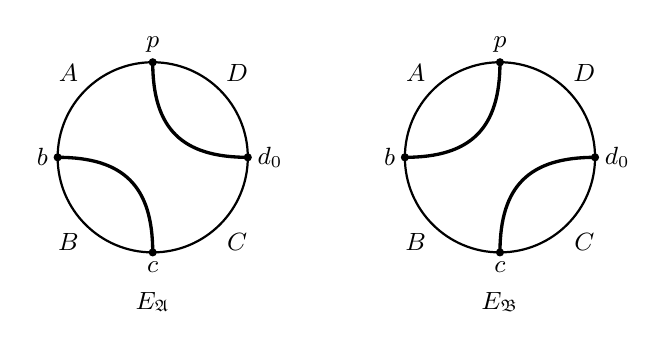
\begin{tikzpicture}[scale=1.05, every node/.style={font=\small}]
\foreach \dx/\ev in {0/{E_{\mathfrak A}},4.2/{E_{\mathfrak B}}}{
  \begin{scope}[xshift=\dx cm]
  \draw[thick] (0,1.15) arc[start angle=90,end angle=450,radius=1.15];
  \foreach \pos/\lab in {(0,1.15)/p,(-1.15,0)/b,(0,-1.15)/c,(1.15,0)/d_0}
    \fill \pos circle[radius=1.4pt];
  \node[above] at (0,1.15) {$p$};
  \node[left] at (-1.15,0) {$b$};
  \node[below] at (0,-1.15) {$c$};
  \node[right] at (1.15,0) {$d_0$};
  \node at (-1.02,1.02) {$A$};
  \node at (-1.02,-1.02) {$B$};
  \node at (1.02,-1.02) {$C$};
  \node at (1.02,1.02) {$D$};
  \node at (0,-1.75) {$\ev$};
  \end{scope}
}
\draw[very thick] (0,1.15) .. controls (0,.35) and (.35,0) .. (1.15,0);
\draw[very thick] (-1.15,0) .. controls (-.35,0) and (0,-.35) .. (0,-1.15);
\begin{scope}[xshift=4.2cm]
\draw[very thick] (0,1.15) .. controls (0,.35) and (-.35,0) .. (-1.15,0);
\draw[very thick] (0,-1.15) .. controls (0,-.35) and (.35,0) .. (1.15,0);
\end{scope}
\end{tikzpicture}
\caption{The two four-port pairings after local caps are attached.
The boundary is drawn as a circle only to show cyclic order; $A,C$
wire $\mathfrak A$ and $B,D$ wire $\mathfrak B$.  Completing around
$A,C$ adds one loop on the left and two on the right.  The thick curves
are open medial strands, not cluster paths.}
\label{four:pairing-figure}
\end{figure}


For later use we make the finite tree computation explicit.  Let $L(e)$
be the number of marks among $b,c,d_0$ in the child boundary interval of
$e$.  Those marks form a consecutive subset.  Their drops are $s,t,s$;
the endpoint high statuses agree when $L$ is odd and differ when it is
even.  Substitution in \eqref{four:edge-weights} gives
\begin{equation}
\begin{array}{c|cc}
 L&w_e&k_e\\ \hline
 0&d,\ 1&-1,\ -d\\
 1\ (b\text{ or }d_0)&1&0\\
 1\ (c)&1&-d\\
 2&1,\ d&0,\ -(d^2-1)\\
 3&0&1
\end{array}
\label{four:table}
\end{equation}
Two entries refer, in order, to a high and a low first port.

The $L>0$ subtree has four terminal legs, possibly of zero length.
The $p$-leg has $L=3$, and the other legs have $L=1$.  Between the
branches is either one shared node or a chain of $m\ge1$ edges with
$L=2$.  A chain of type $X$ encloses $c,d_0$ and has ports on $B,D$;
write $\mathfrak C=\mathfrak B$ in this case.  A chain of type $Y$
encloses $b,c$, has ports on $A,C$, and has $\mathfrak C=\mathfrak A$.
These are the only possibilities because descendant marked sets are
nested.  Number the chain nodes $0,\ldots,m$ away from the $p$-leg,
and write $c_j$ for their colors.  For a shared branch use $m=0$.

Leg and branch nodes are wired: each meets intervals of both designated
colors, also when a leg collapses at a mark.  An internal chain node
meets only intervals wiring $\mathfrak C$, and cannot meet a mark because
its descendant marked set is unchanged along the chain.  The child of
an $L=0$ edge is unwired exactly when its first port is high.  Hence
\begin{equation}
 \mathcal I=\mathcal I_0+\mathcal I_{\rm mid},\qquad
 \mathcal I_{\rm mid}=\#\{0<j<m:c_j\ne\mathfrak C\},
 \label{four:count-split}
\end{equation}
where $\mathcal I_0$ counts high-starting $L=0$ edges.  If $m>0$,
the endpoint regions of each chain edge both visit the two
$\mathfrak C$-intervals, so $E_{\mathfrak C}$ holds.  If $m=0$,
the shared node visits all four intervals, giving the connection of
color $c_0$.  Since a chain edge has $w_e=d$ precisely when its child
has color $\mathfrak C$,
\begin{equation}
 F:=d^{-\mathcal I_{\rm mid}}\prod_{L(e)=2}w_e
 =\begin{cases}
 d^{\mathbf1_{\{c_0\ne\mathfrak C\}}},&m>0,\\
 1,&m=0.
 \end{cases}
 \label{four:F}
\end{equation}
Every off-path $L=0$ weight cancels its contribution to $d^{\mathcal I}$.
Inside an $L=0$ branch contained in $R$, define
\begin{equation}
 g_R(\text{wire color})=\tfrac12,\qquad
 g_R(\text{other color})=-\tfrac12.
 \label{four:g}
\end{equation}
Then
\begin{equation}
 \frac{k_e}{w_e}
 =-d^{g_R(\operatorname{col}(v))-g_R(\operatorname{col}(u))},
 \qquad a_e=A_R.
 \label{four:tail}
\end{equation}
In particular, two successive increments of $H$ in such a branch cancel.

\begin{lemma}[Marked values and corrected observable]
\label{four:marked}
Call the tree \emph{typical} when all four terminal legs have positive
length.  On a typical tree,
\begin{equation}
 D_p=D_b=D_{d_0}=0,\qquad
 \frac{H_b}{P_0G}=\begin{cases}1&E_{\mathfrak A},\\d&E_{\mathfrak B},\end{cases}
 \quad
 \frac{H_{d_0}}{P_0G}=y\begin{cases}d&E_{\mathfrak A},\\1&E_{\mathfrak B}.
 \end{cases}
 \label{four:marked-values}
\end{equation}
On the gap visits of any interval $R$,
\begin{equation}
 \begin{gathered}
 \Re(H_V/A_R)-c_R(\operatorname{col}(V))D_V
 \quad\text{is constant},\\
 c_R(\text{wire color})=-\cos\lambda,\qquad
 c_R(\text{other color})=\cos(2\lambda).
 \end{gathered}
 \label{four:line-invariant}
\end{equation}
Set
\begin{equation}
 \Gamma(\mathfrak A)=P_0y^2,\qquad
 \Gamma(\mathfrak B)=-P_0y,\qquad
 H_V^\circ=H_V-\Gamma(\operatorname{col}(V))D_V.
 \label{four:corrected}
\end{equation}
The variables $H_V^\circ$ are bounded uniformly over all trees and vertices.
On a typical tree they have value $P_0GT$ along the $c$-leg and all its
descendant branches, where
\begin{equation}
 T=\mathbf1_{E_{\mathfrak A}}+y\mathbf1_{E_{\mathfrak B}}.
 \label{four:T}
\end{equation}
On gap visits along $B$, their only possible values are $H_b,P_0GT$;
along $C$, they are $H_{d_0},P_0GT$.
\end{lemma}

\begin{proof}
An unpassed $L=3$ edge kills every term of $H$, so only its last edge
can mark.  Once the first $b$- or $d_0$-leg edge has been passed,
$k_e=0$ kills all later marked terms.  At node $0$,
\begin{equation}
 D=F,\qquad H/P_0=
 \begin{cases}F,&c_0=\mathfrak A,\\-y^3F,&c_0=\mathfrak B.
 \end{cases}
 \label{four:branch-values}
\end{equation}
The first $b$-leg coefficient $a_e/P_0$ is $-y^2$ or $y^{-1}$,
according as the parent color is $\mathfrak A$ or $\mathfrak B$;
the corresponding $d_0$-leg coefficients are $-y^4$ or $y$.
This gives \eqref{four:marked-values} at the near branch or shared node.

On the middle chain, $a_e/P_0=y$ in type $X$ and $-y^2$ in type $Y$.
If the first chain edge has $k_e=0$, its weight is $w_e=1$ and only
that chain mark contributes.  Otherwise $F=d$; the chain terms and
the target mark contribute $(2-d^2)$ times the chain amplitude.
Indeed the second chain edge already has $k=0,w=1$, or, when $m=1$,
the target edge has the same amplitude.  The identities
\begin{equation}
 d+(2-d^2)y=yG,\qquad
 -dy^3-(2-d^2)y^2=G
 \label{four:far-algebra}
\end{equation}
give the far-branch values; the first-$k=0$ cases give the same values.

For \eqref{four:line-invariant}, consider first the earlier port of an
arc, and let $r=1$ for a high port and $r=-1$ otherwise.  With
``before'' and ``after'' referring to boundary-gap visits,
\begin{equation}
 \Re(a_e/A_R)=\cos((m_e-r\Delta)\lambda)
       =c_{\rm after}k_e-c_{\rm before}w_e.
 \label{four:early-port}
\end{equation}
At the later port, using its own high status,
\begin{equation}
 -\Re(a_e/A_R)=-\cos((m_e+r\Delta)\lambda)
       =c_{\rm after}w_e-c_{\rm before}k_e.
 \label{four:late-port}
\end{equation}
These product-to-sum identities and \eqref{four:recursion} prove the
invariant, including across a corner in the same interval.

For $R=B,C$, direct substitution gives
\begin{equation}
 \Re(\Gamma/A_R)=c_R,\qquad
 d\Gamma(\text{wire color})+\Gamma(\text{other color})=-A_R.
 \label{four:Gamma-identities}
\end{equation}
Thus $H^\circ$ is unchanged on $L=0$ edges in $B,C$.  It is unchanged
on $c$-leg edges as well: those have $w=1,k=-d$, and $a=A_C$ for
a high first port, whose parent color is $\mathfrak B$, and $a=A_B$
otherwise.  The table bounds all other parts of the tree: an unpassed
$p$-leg kills terms; the middle chain kills a complete prefix in at most
two steps; and an $L=0$ tail has the two-step rule
\eqref{four:tail}.  The $c$-leg is the only place where the uncorrected
variables can grow, and the correction is constant there.  This proves
the uniform bound for $H^\circ$, including atypical trees.

At a node incident to a $c$-leg edge, the $B,C$ line invariants,
anchored by \eqref{four:marked-values}, intersect at $P_0GT$ when $d>1$.
The four line directions after division by $P_0G$ are
\begin{equation}
 1,\quad -y^{-1},\quad y^2,\quad -y
 \qquad\text{on }A,B,C,D,
 \label{four:directions}
\end{equation}
as follows from $iA_R/(P_0G)$ up to nonzero real factors.  At $d=1$
the same identity follows by continuity for each fixed finite tree.
The descendants beyond a $c$-leg edge lie in its $B,C$ boundary disk;
its $L=0$ side branches therefore preserve this value.

The gap walk along $B$ goes from the end of the $b$-leg to the end
of the $c$-leg.  Its $L=0$ excursions preserve $H^\circ$, so only
type-$X$ middle nodes need checking.  Similarly only type-$Y$ nodes
need checking for $C$.  At node $0$,
\begin{equation}
 H^\circ/(P_0G)=F\quad(c_0=\mathfrak A),\qquad
 H^\circ/(P_0G)=yF\quad(c_0=\mathfrak B).
 \label{four:corrected-branch}
\end{equation}
After the first zero $k$, the value stays at the far-branch value.
If the first $k$ is nonzero, the first jump is $-y^{-1}$ in type $X$
with $c_0=\mathfrak A$, and $-y^2$ in type $Y$ with
$c_0=\mathfrak B$.  Thus node $1$ already has value $T$ in normalized
units.  These are precisely the alternatives in the statement.
\end{proof}

\subsection{Moments, shielding, and disappearance of the diagonal term}

The tree calculation gives the marked values and the corrected values
along each boundary interval.  To pass these statements to subsequential
limits, we need moment bounds and boundary shielding, followed by
cancellation of the diagonal residual.

\begin{lemma}[Compactness and boundary shielding]
\label{four:compactness}
For every fixed positive power, the moments of $|H_{V(z)}|+|D_{V(z)}|$
are bounded by a power of $\min(1,|z-c|)^{-1}$, uniformly when $z$
is farther than a mesh-scale distance from $c$.  The expectations in
\eqref{four:observable} are asymptotically equicontinuous on interior
compact sets.  Every lattice parity therefore has the same locally
continuous subsequential limits.

Typicality has probability tending to one.  As a macroscopic interior
point approaches an ordinary boundary point, including a polygon corner,
its tree vertex visits that point's interval with probability tending to
one after the mesh limit.  Near $b,c,d_0$ it lies beyond an edge of the
corresponding terminal leg with high probability; near $p$ an unpassed
$L=3$ edge remains with high probability.
\end{lemma}

\begin{proof}
The table and the two-step cancellation bound $|H_V|+|D_V|$ by
$C\exp(C\ell)$, where $\ell$ is the number of $c$-leg edges passed
on the root-to-$V$ path.  A passed $c$-leg arc has a child disk containing
$z$.  It cannot be wholly inside a box at $c$ of radius a small fixed
multiple of $\min(1,|z-c|)$, because the flat wall makes such a child
disk local.  Fixed buffers and the dyadic bands between that radius and
macroscopic scale count these passages.  The conditional passage
estimates of Lemmas~\ref{prelim:passages} and~\ref{prelim:tilts}, grouped into disjoint
buffer colors, give the asserted moments.  Bounded open-cap reweighting
allows their use under a deterministic-cap FK law.  If two nearby
interior vertices have different boundary-tree regions, a raw boundary
arc travels from their vicinity to the wall.  Bulk RSW circuits make
this probability uniformly small; H\"older's inequality and the moment
bound give equicontinuity, including between lattice parities.

For the boundary claims, work on separated scales in the relevant wall
sector.  In disjoint buffers impose two actual wall-to-wall crosscuts,
of opposite colors, the first inside the second.  Up-to-wall RSW gives
a uniform conditional lower bound.  A raw medial separator lies between
the two thickened paths and joins the two banks.  One direct verification
is to trace the perimeters: on either bank the gaps at the two crosscut
ends have opposite colors, so an odd number of ports lies between them;
the paths prohibit radial escape, and at least one of these ports must
be paired to the other bank.  Such an arc separates the deeper box
from the exterior.  The same argument works in a corner sector.
Iteration gives probability tending to one at diverging scale ratio.
It produces the claimed local raw arch at an ordinary point and the
appropriate terminal-leg separator at each mark.
\end{proof}

\begin{lemma}[Diagonal residual cancellation]
\label{four:residual}
For every bounded function $\gamma$ of the two colors and every boundary
point $u$ distinct from the four marks,
\begin{equation}
 \lim_{z\to u}\limsup_{n\to\infty}
 \left|\mathbb E_{\rm open}
       [\gamma(\operatorname{col}(V(z)))D_{V(z)}]\right|=0.
 \label{four:boundary-residual}
\end{equation}
Here $z$ in the outer limit is a macroscopic interior location, and any
lattice vertices tending to it may be used in the inner limit.
\end{lemma}

\begin{proof}
We first cancel a positively weighted residual at a fixed interior $z$.
Replace the marked primitive by the full $K(Q)$ string from $p$ to $z$.
If $N$ is the number of internal closed loops surrounding $z$, their
weight ratio is $-2/d$.  Let $\sigma$ take opposite signs on the two
colors.  Nesting parity gives
$(-1)^N=\sigma(\operatorname{col}(z))\sigma(\operatorname{col}(V))$.
Equality of the two winding expansions implies
\begin{equation}
 \mathbb E_{\rm open}
       [\sigma(\operatorname{col}(V))D_V(2/d)^N]=o(1).
 \label{four:weighted-residual}
\end{equation}
Here is the required absolute estimate in the wrong expansion.
Relative to the complementary cap partition it is at most
\begin{equation}
 K_*^{1+X_*}
 \prod_{\nu=p,b,d_0}\mathbf1_{\{N_\nu=0\}}\,
 d^{N_c}\prod_{v\text{ a corner}}f(g_v)^{N_v/2},
 \qquad g_v\in\{-\tfrac12,\tfrac12\}.
 \label{four:wrong-bound}
\end{equation}
The counts use disjoint small macroscopic cutoffs.  The variable $X_*$
counts macroscopic passages and has every fixed exponential moment;
its constants may depend on $z$.  Away from singularities, ordinary
small arcs have the complementary zero-drop cap weights.  At $b,d_0,c$
the effective wrong drops are $-s,-s,-t$, with weights $0,0,d$.
At $p$, use a locally forward boundary interval.  Its arc meets the
exiting string with net intersection $-1$; after changing the winding
convention the effective drop is $s+1$, again giving weight zero.
This depends on the net intersection, not the placement of the string.
Corner alternation and cap elimination give the remaining factors in
\eqref{four:wrong-bound}.  Internal loops around $z$ have absolute
weight $2|\cos(2\lambda)|\le d$, and each nonlocal arc costs at most
a bounded factor per passage.

Without the $K_*^{1+X_*}$ factor, the logarithm of the expectation is
bounded above by
\begin{equation}
 3P+D_*+\sum_{v\text{ convex}}C_{i(v)}
          +\sum_{v\text{ concave}}L_{i(v)}+O(1).
 \label{four:residual-budget}
\end{equation}
Let $Y_n$ be the nonnegative product in \eqref{four:wrong-bound}
without $K_*^{1+X_*}$.  Its second moment is polynomial in $n$.
For $0<\eta<1$, H\"older and interpolation between its first two
moments give
\[
 \mathbb E[Y_nK_*^{1+X_*}]
 \le C_\eta(\mathbb E Y_n)^{(1-\eta)/(1+\eta)}
             (\mathbb E Y_n^2)^{\eta/(1+\eta)}.
\]
The constant uses the fixed exponential moment of $X_*$ at rate
$(1+\eta)\log K_*/\eta$.  The budget in
\eqref{four:residual-budget} has size $O(\log n)$, so this costs only
$O(\eta\log n)$ in that upper bound; no lower bound on
$\mathbb E Y_n$ is needed.  The balanced-corner budget
\eqref{exp:polygon-saving} is strictly negative by
\eqref{exp:strict-arm}.  Our global color choice makes the complementary
cap partition at most a constant times the correct open-cap partition.
This proves \eqref{four:weighted-residual}.

We next remove the positive weight, retaining relative error estimates.
Let $\mu$ be the correct deterministic-cap FK law and
$R_*=d^{\ell_{\rm open}-\ell_{\rm det}}$; open expectation is
$\mathbb E_\mu[R_*\cdot]/\mathbb E_\mu R_*$.  For the interval $R$
containing $u$, put
\begin{equation}
 B_*=R_*\sigma(\operatorname{col}(V))
             d^{-g_R(\operatorname{col}(V))}D_V,
 \qquad
 T_*=d^{g_R(\operatorname{col}(V))}(2/d)^N.
 \label{four:BT}
\end{equation}
Thus $\mathbb E_\mu[B_*T_*]=o(1)$ at every fixed $z$.
Choose scales in the regular sector at $u$ with
\begin{equation}
 |z-u|\ll r_1\ll r_2\ll r_3\ll1,
 \label{four:residual-scales}
\end{equation}
all ratios diverging as $z\to u$, and take the mesh limit first.

Except on an event of vanishing probability, $B_*$ is determined outside
$r_2$.  To see this, use actual screens to ensure that no raw strand
from the $r_2$ rim reaches $r_3$.  Every changing boundary arc then lies
in one small part of $R$, so has $L=0$.  All $L>0$ data, the marked
subtree and $R_*$ are fixed.  Regard arcs touching the connected patch
as affected and arcs wholly outside it as stable.  Stable separators
either separate the entire patch from $p$ or do not; noncrossing puts
the affected on-path arcs after them.  Off-path factors cancel, while
the on-path $k/w$ suffix telescopes by \eqref{four:tail}.  The color
factor in $B_*$ cancels that suffix exactly.  Set $B_{\rm out}=B_*$
on this exterior good event and zero otherwise.

Truncate $T_*$ to $T_{\rm in}$ by counting only enclosing loops wholly
inside $r_1$ and reconstructing the tree color from their parity and the
fixed lattice color of $z$.  This is exact unless a raw path runs from
$O(|z-u|)$ to the $r_1$ scale: every enclosing loop meets the segment
from $z$ to its nearest wall point.  To measure both truncation errors,
let $N_0$ count the enclosing loops wholly inside the box of radius
$\operatorname{dist}(z,\partial\Omega)/8$ at $z$, and put
$U_z=(2/d)^{N_0}$.  Work under the positive tilt
$\nu_{U_z}\propto U_z\mu$.  The rare events remain rare under this
tilt by conditional RSW outside its support.  The variables $B_*$,
$T_*/U_z$, and $T_{\rm in}/U_z$ have uniformly bounded fixed moments
as $z\to u$.  For $B_*$, every relevant $c$-leg arc gives a macroscopic
passage away from $u$; an arc wholly local at $u$ would have $L=0$.
Every extra loop in $T_*$ gives a passage in a band at distance comparable
to $\operatorname{dist}(z,\partial\Omega)$, by the segment observation
and its escape from the cutoff.  Finitely many bulk and sector buffers
cover this band uniformly.  Near a corner, use a corner buffer and small
straight-bank buffers, or only the latter if the corner is farther away
than this scale.  The tilt-edge passage estimates apply in each buffer.
H\"older therefore makes the product truncation errors
$o(\mathbb E_\mu U_z)$, and
\begin{equation}
 \mathbb E_\mu T_{\rm in}\asymp\mathbb E_\mu U_z\ge1.
 \label{four:T-comparison}
\end{equation}

The inward relative comparison of Lemma~\ref{prelim:relative-collar}
between $r_1$ and $r_2$, applied
to this positive inner factor and the absolute parts of $B_{\rm out}$,
gives
\begin{equation}
 \frac{\mathbb E_\mu[B_{\rm out}T_{\rm in}]
 -\mathbb E_\mu B_{\rm out}\,\mathbb E_\mu T_{\rm in}}
 {\mathbb E_\mu U_z}=o(1).
 \label{four:relative-decoupling}
\end{equation}
This is the one-sector case of that lemma: the two side rays carry
the common primal wire when $R$ is primal, and there are no through
primal wires when $R$ is dual.
First use \eqref{four:weighted-residual} at fixed $z$, then let $z\to u$.
Equations~\eqref{four:T-comparison}--\eqref{four:relative-decoupling}
show that $\mathbb E_\mu B_*$ vanishes in this order of limits.
Finally apply the same separation without a tilt to $B_*$ times any
bounded function of the tree color, reconstructing that color from the
inner-loop parity.  Its expectation factors up to $o(1)$ into
$\mathbb E_\mu B_{\rm out}$ and a bounded inner expectation.
Taking the bounded color factor that reverses the extra factors in
\eqref{four:BT}, and dividing by $\mathbb E_\mu R_*$, proves
\eqref{four:boundary-residual}.
\end{proof}

\subsection{The boundary problem, conditional on holomorphicity}

\begin{proposition}[Identification of a holomorphic subsequential limit]
\label{four:conditional-map}
Suppose an interior subsequential limit $h$ of $h_n$ is holomorphic in
the ordinary complex coordinate, and pass simultaneously to a limit
$r$ of $P_{\mathfrak A}$.  Then $0<r<1$.  Put
\begin{equation}
 U_0=r+d(1-r),\qquad V_0=dr+1-r,\qquad T_0=r+y(1-r).
 \label{four:target-vertices}
\end{equation}
The function $h$ maps $\Omega$ conformally onto the interior of the
simple polygon with successive vertices $0,U_0,T_0,yV_0$, taking
$p,b,c,d_0$ to those vertices.  If a conformal half-plane coordinate
takes the marks to $0,\chi,1,\infty$, respectively, then
\begin{equation}
 r=\frac{\displaystyle\int_1^\infty
        u^{\rho-1}|u-\chi|^{\rho-1}|u-1|^{1-3\rho}\,du}
       {\displaystyle\int_\chi^\infty
        u^{\rho-1}|u-\chi|^{\rho-1}|u-1|^{1-3\rho}\,du}.
 \label{four:crossing-formula}
\end{equation}
Under deterministic separate $\mathfrak A$ caps the corresponding
crossing probability is $r/(r+d(1-r))$.
\end{proposition}

\begin{proof}
Fixed up-to-wall RSW corridors give both actual crossings positive
probability under deterministic caps, and hence under open caps;
thus $0<r<1$.  Shielding and the moment bounds give the interior
limits $0,U_0,yV_0$ at $p,b,d_0$: near $p$ an unpassed $L=3$ edge
kills $H$, and near $b,d_0$ the first $k=0$ edge fixes it at its marked
value.  At every other boundary point the line invariant, shielding,
and Lemma~\ref{four:residual} put $h$ on the corresponding line of
direction \eqref{four:directions}, with offsets fixed by these values.
In a conformal half-plane coordinate, whose boundary extension is
homeomorphic, the line-normal harmonic component vanishes continuously
on each unmarked interval.  Harmonic Schwarz reflection, followed by
extension of its harmonic conjugate, extends $h$ holomorphically across
that interval.

On $B,C$ the traces lie on the actual segments
$[U_0,T_0]$ and $[T_0,yV_0]$, respectively.  Indeed $H^\circ$ has,
for each connection event, only the two values in
Lemma~\ref{four:marked}; the segment direction is fixed, so averaging
keeps it between the averaged endpoints.  Its correction has zero
limiting expectation at every fixed boundary point.  As that point
approaches $c$, shielding gives a $c$-leg separator enclosing it and
nearby interior points.  The uniform bound for $H^\circ$ therefore
makes the boundary trace tend to $T_0$.

There is also continuity at $c$ from the interior.  In a half-plane
coordinate $\zeta$ with $c=0$, the flat wall and the moment bounds
give polynomial growth of $h-T_0$.  Its two boundary directions are
$-y^{-1}$ on the negative and $y^2$ on the positive real axis.
Consequently
\begin{equation}
 e^{-2i\lambda}\zeta^{3\rho-1}(h(\zeta)-T_0)
 \label{four:corner-reflection}
\end{equation}
has real boundary values on both sides, with the branch in the upper
half-plane.  Schwarz reflection makes it holomorphic on a punctured
disk; polynomial growth makes its singularity at worst a pole.
Its leading Laurent power, after undoing the multiplier, must have
positive exponent because the two boundary traces tend to zero.
Thus $h\to T_0$ throughout the interior approach as well.

The target polygon is counterclockwise and simple.  For $d>1$ its
vertex $T_0$ is reflex: in the basis $1,y$ it lies strictly inside the
triangle with vertices $0,U_0,yV_0$.  When $d=1$, it lies on the
third side of that triangle.  For any point off the four boundary
lines, straighten each continuous boundary trace in its own line.
Its winding number is that of the target polygon.  The argument
principle therefore gives one preimage of every generic interior
point and none of every generic exterior point.  The open mapping
theorem puts the open image inside the polygon, and then the traces
on $A,D$ also lie on their actual segments.  The segment control on
$B,C$ already established is needed at the reflex corner.  No interior
point lies on the trace, and the preimage count proves conformal
bijectivity.

The four target angles are
$\rho\pi,\rho\pi,(2-3\rho)\pi,\rho\pi$.  The
Schwarz--Christoffel formula therefore has derivative proportional to
$\zeta^{\rho-1}(\zeta-\chi)^{\rho-1}(\zeta-1)^{1-3\rho}$;
see, for example, \cite{Pommerenke1992}.  The $B$ and $C$ side vectors
are $-(1-r)y^{-1}$ and $ry^2$, so their lengths are $1-r$ and $r$.
Their ratio gives \eqref{four:crossing-formula}.  At $d=1$ the straight
marked point has exponent zero, as required.  Lemma~\ref{four:tree}
reweights the two open-cap alternatives by $d$ and $d^2$, giving the
last assertion.
\end{proof}

For $q=1$, one has $d=1$, $\rho=1/3$, and the substitution $v=\chi/u$
turns \eqref{four:crossing-formula} into Cardy's integral
\cite{Cardy1992}.  No boundary-law reweighting of actual paths is then
needed.  Holomorphicity and the boundary approximation transfers are
still required before this conditional computation becomes a scaling
limit statement.

\section{Paired walls and distant charges}
\label{sec:pairedwall}

We now put a source primitive on each bank of the polygon wall.  The
purpose of the exterior source is to leave a nonconstant second factor
after applying a mixed bulk estimate; no conformal invariance of the
exterior probability law is used.

\subsection{The paired-wall tensor and its normalization}

Let $O=\mathbb C\setminus\overline\Omega$.  At every used wall port,
replace the ordinary spin contraction by the product of two boundary
factors.  Use the same factor $b_i$ on the interior and exterior banks,
each evaluated on the arrow sign relative to that bank's inward normal.
The exterior designated color is opposite to the interior one.
Starting at $p$, the exterior order is $D,C,B,A$, and the high statuses
on the two banks agree.  Its physical normal lift is
$\theta_O=\theta_\Omega+\pi$, has total turn $-2\pi$, and has raw
bases $H_R-\tfrac12$.

Take the two source primitives from $p$ to $z\in\Omega$ and from $p$
to $u$ in an exterior collar strip along $D$.  The strip is connected
and simply connected and approaches both $p$ and $d_0$; initially
we restrict $u$ to its interior compact sets.  Use the respective
inward initial lifts.  A \emph{pure string of charge $a$} along a
directed tile path contributes $e^{i\lambda ac}$ at a crossed spin,
where $c=1$ denotes an arrow in the path's left-normal direction.
Add the following strings:
\begin{enumerate}[label=(\roman*),leftmargin=*]
\item In exterior boundary order put
\begin{equation}
 P_D=0,\quad P_C=-2s,\quad P_B=-2(s+t),\quad P_A=-2(2s+t).
 \label{wall:short-charges}
\end{equation}
For each nonzero $P_R$, run a charge-$P_R$ string forward, parallel
to its interval in boundary homotopy, with its endpoints at the interval
ends and its interior off the wall.  Sliding this path out through a
complete wall adds $P_R$ to that interval's raw base.
\item Choose two finite sets of positive numbers $a_j$, each with sum
$1$, satisfying $a_j<1$ and $(1+a_j)\lambda<\pi/2$.
Run charge-$(-a_j)$ strings from $p$ to exterior bulk vertices $w_j$,
at successively separated distances
\begin{equation}
 r_j\asymp R_0L^{j-1}
 \label{wall:distant-scales}
\end{equation}
from a fixed pole $z_*\in\Omega$.  Their initial portions follow a
common simple cut from $p$ out to distant scales before splitting;
they never return near the polygon.  Continue this cut notionally to
infinity, and back through $\Omega$ to $z_*$.
\end{enumerate}
First fix a sufficiently large $L$, then let $R_0$ become large after
the mesh limit.  Exterior probe paths stay on the starting $D$ side
of the cut and avoid the short strings and their sliding homotopies.
To arrange this, choose thin topological boundary strips separated
at the marks by sector curves, reserve the $D$ strip for probes, and
send the cut out at $p$.  Each fixed geometry admits piecewise smooth
paths with clear corridors and then tile-edge approximations.
Figure~\ref{wall:geometry-figure} shows the two probe regions and the
common outgoing cut before its distant branches separate.

\begin{figure}[htbp]
\centering
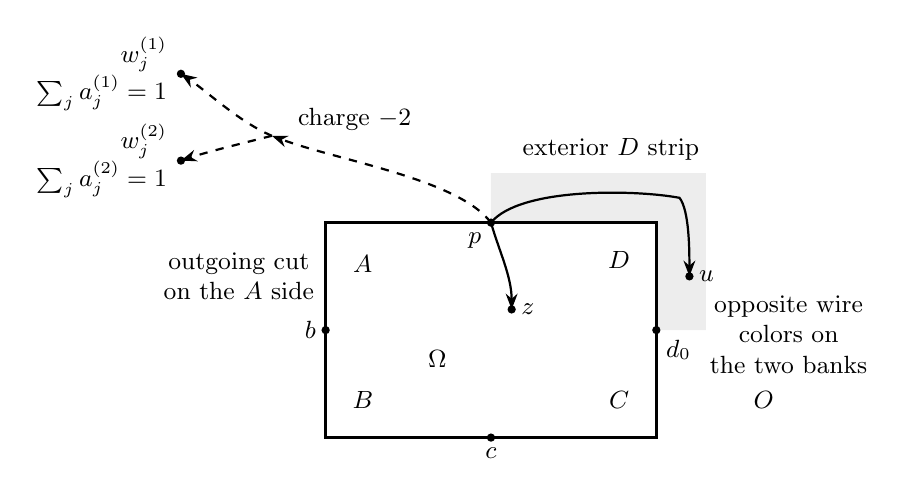
\begin{tikzpicture}[x=1.05cm,y=1.05cm,
  every node/.style={font=\small},
  source/.style={thick,-{Stealth[length=2mm]}},
  charge/.style={thick,dashed,-{Stealth[length=2mm]}}]
\fill[gray!14] (0,1.3) -- (2,1.3) -- (2,0)
  -- (2.6,0) -- (2.6,1.9) -- (0,1.9) -- cycle;
\draw[very thick] (-2,-1.3) rectangle (2,1.3);
\node at (-.65,-.35) {$\Omega$};
\node at (3.3,-.85) {$O$};
\node at (-1.55,.8) {$A$};
\node at (-1.55,-.85) {$B$};
\node at (1.55,-.85) {$C$};
\node at (1.55,.85) {$D$};
\foreach \point in {(0,1.3),(-2,0),(0,-1.3),(2,0)}
  \fill \point circle[radius=1.5pt];
\node[below left] at (0,1.3) {$p$};
\node[left] at (-2,0) {$b$};
\node[below] at (0,-1.3) {$c$};
\node[below right] at (2,0) {$d_0$};
\draw[source] (0,1.3) .. controls (.1,.95) and (.25,.65) .. (.25,.25);
\fill (.25,.25) circle[radius=1.5pt];
\node[right] at (.25,.25) {$z$};
\draw[source] (0,1.3) .. controls (.35,1.73) and (1.75,1.7) .. (2.28,1.6)
  .. controls (2.4,1.45) and (2.4,.95) .. (2.4,.65);
\fill (2.4,.65) circle[radius=1.5pt];
\node[right] at (2.4,.65) {$u$};
\node[above,align=center] at (1.45,1.93) {exterior $D$ strip};
\draw[charge] (0,1.3) .. controls (-.4,1.83) and (-1.85,2.05) .. (-2.65,2.35);
\draw[charge] (-2.65,2.35) .. controls (-3.05,2.52) and (-3.45,2.9) .. (-3.75,3.1);
\draw[charge] (-2.65,2.35) .. controls (-3.05,2.25) and (-3.45,2.15) .. (-3.75,2.05);
\fill (-3.75,3.1) circle[radius=1.5pt];
\fill (-3.75,2.05) circle[radius=1.5pt];
\node[left,align=right] at (-3.8,3.1)
  {$w_j^{(1)}$\\$\sum_j a_j^{(1)}=1$};
\node[left,align=right] at (-3.8,2.05)
  {$w_j^{(2)}$\\$\sum_j a_j^{(2)}=1$};
\node[above] at (-1.65,2.3) {charge $-2$};
\node[align=center] at (-3.05,.65) {outgoing cut\\on the $A$ side};
\node[align=center] at (3.6,-.05)
  {opposite wire\\colors on\\the two banks};
\end{tikzpicture}
\caption{The paired-wall geometry in the original plane.  The solid
arrows are the two source paths from $p$; the exterior probe stays in
the shaded strip along $D$.  The dashed pure strings leave on the
other side of $p$.  Each of their two endpoint lists has total charge
$-1$, so their common initial cut has charge $-2$.  Only representative
distant endpoints are shown, not their separated metric scales.
The polygon is schematic; the short interval strings and the fine
parallel lanes at $p$ are omitted.  Inversion is used only to describe
the ideal exterior turn factors, not to change its probability law.}
\label{wall:geometry-figure}
\end{figure}


At shared initial tile edges use ordered parallel lanes, with pure
strings on the non-probe side when they separate.  This specifies the
matrix order: the lanes cross the same smooth raw strand near a port
midpoint, and diagonal phases act on the specified side of $L_-$.
Near tile vertices they can be joined without extra strand crossings.
Pure lanes need no mutual ordering.  Source paths may be chosen in
fixed homotopy with continued lift throughout their domains, also when
small wall gaps are present away from the marks and these corridors.

For a positive reference law, cap each designated primal interval
separately on each wall component.  At a fragment tip the designated
color changes between banks.  Write $\mu$ for this deterministic-cap
FK law, and $Z^{\rm cap}$ for its all-loop partition relative to the
uncut plane vacuum, including common tile coefficients.  If
$\Xi(z,u)$ denotes the vacuum spin expectation of the boundary factors,
sources, and pure strings, the winding expansion gives
\begin{equation}
 \frac{\Xi(z,u)}{Z^{\rm cap}}
       =\mathbb E_\mu\mathcal O(z,u),
 \label{wall:diagram-normalization}
\end{equation}
where $\mathcal O$ is the oriented diagram sum divided, configuration
by configuration, by the deterministic-cap loop weight.  All changes
are finite at each mesh.  The almost-sure finiteness of vacuum loops,
or the finite-cylinder construction of Section~\ref{sec:angular},
justifies this identity even in the plane; unchanged remote loops have
ratio one after orientation summation.

For each $j$, let $N_j$ count closed raw loops surrounding $w_j$ wholly
inside a box of a fixed small relative radius at scale $r_j$.  Set
\begin{equation}
 U=\prod_j u_+(a_j)^{N_j},\qquad
 u_+(a)=\frac{\cos((1+a)\lambda)}{\cos\lambda}>0.
 \label{wall:U}
\end{equation}
The patches are disjoint and buffered.  For gapped walls a further
positive tip factor $T_g$ will be introduced in
Section~\ref{sec:closinggaps}; it equals $1$ for a complete wall.
The normalized paired-wall function is
\begin{equation}
 \mathcal H_g(z,u)=
 \frac{\Xi_g(z,u)}{Z_g^{\rm cap}\mathbb E_{\mu_g}[UT_g]}.
 \label{wall:H-normalized}
\end{equation}

\subsection{The ideal exterior observable and its phases}

With a complete wall, the capped interior and exterior are independent
by the loop weights and domain Markov property.  The interior factor
is $h_n(z)$ times $c_*P_0G$ and the bounded ratio of its open and
deterministic-cap partitions.  The ideal exterior object is the same
four-change disk-tree observable on $O\cup\{\infty\}$, viewed after
inversion about $z_*$: its boundary order is $D,C,B,A$, its bases in
that order are $(s+1,1,s,0)$, its launch is $p$, and it uses the exterior
high designation.  Raw boundary arcs form a finite disk tree, since
none escapes to infinity almost surely.  This definition needs no
tiles at infinity and does not change the exterior positive law.
Write $H^O_{V_O(u)}$ for the tree variable \eqref{four:H} with these
exterior data, and set
\begin{equation}
 J_n(u)=\frac{\mathbb E_{{\rm open},O}H^O_{V_O(u)}}{P_0G}.
 \label{wall:ideal-observable}
\end{equation}
As for $h_n$, this is the exterior primitive contraction divided by
its open-cap partition and by $c_*P_0G$; the tree variable has already
had the common source factor $c_*$ removed.

The tree table gives local boundedness and asymptotic equicontinuity of
$J_n$ in the probe strip.  A relevant nonlocal arc has a macroscopic
passage near the bounded wall, and separating nearby probe points
requires a boundary-reaching arm.  Shielding at the flat marks gives
limit zero at $p$ and a value bounded away from zero at $d_0$.
Consequently every locally uniform subsequential limit $J$ is continuous
and nonconstant on this connected strip.

The physical phases agree with the ideal ones for bounded open arcs.
First slide the short strings onto the complete wall, avoiding the
source path.  The new raw profile $H_R-\tfrac12+P_R$ differs from the
desired exterior profile by the global constant $-s-\tfrac32$.
Since there is one outward source, this contributes only a fixed phase.
Let
\begin{equation}
 \psi=\arg\left(\left(\frac1{z-z_*}\right)'\right)
 \label{wall:inversion-angle}
\end{equation}
with the cut and continuous lift just chosen.  The inverted normal is
$\theta_O+\psi$ and has total turn $2\pi$: on the clockwise exterior
lap, $\psi$ gains $4\pi$ before the cut is reset.  An oriented arc's
image turn is its physical turn plus the endpoint $\psi$ difference,
minus $4\pi$ times its signed intersections with the outward cut.
Boundary normal factors cancel the endpoint terms.  For a marked arc,
the two departing pieces have additional start terms, canceled exactly
by the change of the gauge $e^{i\rho\alpha}$ at the source.
Prefix intersections are unchanged topologically.  Before the distant
strings split, their total charge is $-2$, which supplies precisely the
remaining image multiplier.  Thus the physical and ideal open-arc
factors agree up to one common phase whenever those arcs stay before
the splitting scales.  This is a calculation with turn lifts of smooth
disjoint drawn arcs, independent of any invariance of their law.

\subsection{A nonzero distant factor}

For a closed exterior loop $\gamma$, let
$A_\gamma=\sum_{w_j\text{ inside }\gamma}a_j$, using its physically
bounded inside.  Such a loop surrounds $p$ exactly when it surrounds
the whole wall.  Its ratio to the ordinary weight is
\begin{equation}
 \begin{cases}
 v(A_\gamma)=\cos((A_\gamma-1)\lambda)/\cos\lambda,
       &\gamma\text{ surrounds the wall},\\
 u(A_\gamma)=\cos((1+A_\gamma)\lambda)/\cos\lambda,
       &\text{otherwise}.
 \end{cases}
 \label{wall:closed-ratios}
\end{equation}
These formulas follow by counterclockwise intersection with the strings.
A closed loop cannot separate the source of a nonzero open-arc term
from the connected wall.  Thus \eqref{wall:closed-ratios} lists all
changes to its weight, including when some open arcs go far.
Let $Y$ be the product of these ratios; only finitely many are nontrivial.

\begin{lemma}[Distant normalization]
\label{wall:distant}
For sufficiently large fixed $L$, under the exterior positive tilt
$\nu_U\propto U\mu$,
\begin{equation}
 \mathbb E_{\nu_U}(Y/U)\ge c_L>0,\qquad
 \mathbb E_{\nu_U}|Y/U|^p\le C_{p,L}
 \label{wall:distant-moments}
\end{equation}
for every fixed $p>0$, uniformly for large $R_0$ and fine mesh.
\end{lemma}

\begin{proof}
Between consecutive endpoint scales use corridor annuli with radii
$Kr_j$ and $r_{j+1}/K$, for a large fixed geometric constant $K$.
Each winding loop wholly in corridor $j$ has ratio
$v(\sum_{i\le j}a_i)\ge1$, because the total charge magnitude is $2$.
Let $M_j$ be the product of these ratios and $M=\prod_jM_j$.
Besides the $U$ nests and these corridor loops, all nontrivial loops
are counted by a variable $X$ having every fixed exponential moment
uniformly under $\nu_U$, with constants independent also of sufficiently
large $L$.  Indeed a loop excluding $z_*$ but surrounding an endpoint
outside its local cutoff has a passage at that endpoint scale, since it
separates the endpoint from $z_*$.  A loop winding about $z_*$ and
enclosing some but not all endpoints either lies in its corridor or
passes a bordering scale.  Fixed box and shell covers, disjoint from
other endpoint buffers, and the tilt-edge passage estimates give the
claim.  Therefore, for a fixed $C$,
\begin{equation}
 |Y/U|\le MC^X,\qquad
 Y/U\ge MC^{-X}\quad\text{off }\mathcal B,
 \label{wall:MY}
\end{equation}
where $\mathcal B$ is the event that some loop excluding $z_*$ encloses
at least two endpoints.  Off $\mathcal B$, all remaining ratios belong
to a fixed finite positive set.  Moreover
\begin{equation}
 \mathbb E_{\nu_U}M^b\le C_bL^{C_b}\qquad(b>0\text{ fixed}).
 \label{wall:M-moments}
\end{equation}
To prove this, use $O(\log L)$ dyadic passage bands per corridor,
group disjoint buffers by colors, and apply H\"older; those buffers
avoid the supports of the endpoint tilts.

If a bad loop has smallest enclosed endpoint index $j$, it crosses
corridor $j$ radially, and hence excludes every winding loop counted
by $M_j$.  Write $\mathcal B_j$ for this event.  Successive actual
circuit blockers give
$\mathbb P(\mathcal B_j\mid U\text{ patches},(M_i)_{i\ne j})
\le CL^{-\alpha}$, uniformly.  On $\mathcal B_j$ one has $M_j=1$.
First apply this conditional estimate to
$\prod_{i\ne j}M_i$, then H\"older with exponent $1+\delta$ close
to one to absorb $C^X$, interpolating against the polynomial moment
bound \eqref{wall:M-moments}.  For some $\alpha'>0$ independent of $L$,
\begin{equation}
 \mathbb E_{\nu_U}[MC^X\mathbf1_{\mathcal B}]
       \le C'L^{-\alpha'}\mathbb E_{\nu_U}M.
 \label{wall:bad-relative}
\end{equation}
The same interpolation, using arbitrary fixed exponential rates for
$X$, gives for every $\varepsilon>0$
\begin{equation}
 \mathbb E_{\nu_U}[MC^{-X}]
       \ge c_\varepsilon L^{-\varepsilon}\mathbb E_{\nu_U}M.
 \label{wall:positive-relative}
\end{equation}
Equivalently, Jensen under the $M$ tilt and the exponential bounds
give an arbitrarily small coefficient of $\log L$ in its mean of $X$.
Take $\varepsilon<\alpha'$ and then $L$ large.  Equations
\eqref{wall:MY}--\eqref{wall:positive-relative}, and $M\ge1$, prove
the positive lower bound in \eqref{wall:distant-moments}.  Its moment
bound follows from \eqref{wall:MY}, \eqref{wall:M-moments}, and H\"older.
\end{proof}

\subsection{Absolute source bounds and factorization}

We record the source-path placement used here and in gap closure.
Both paths can be taken in regular simple tubes, on their nominal
sides of the wall except at the flat launch.  For an absolute estimate,
temporarily slide the exterior pure-string endpoints at $p$ a small
macroscopic distance toward the non-probe, $A$ side of the same solid
wall.  Keep all gaps and other marks farther away, and include the
charge along the traversed bank interval as diagonal port phases.
This is an equality of the summed pairing expression: ordered lanes
allow a homotopy onto the bank without crossing a source path, and
ice conservation gives the port phases.  Pure lanes may cross one
another.  Charges still count from their original endpoints, so no
extra charge is created at a temporary slide-end.  The paired factors
and the conventions used for gluing do not change.

After this temporary slide each tube has $p$ in the relative interior
of a flat entrance face, with a clear portion on both sides; its target
is deep inside, and its other sides avoid the wall, strings, and the
other tube.  Finitely many such choices cover compact probe sets.
For each pairing, choose a path that crosses minimally the disjoint
raw crosscuts of its tube.  A sufficiently small separating crosscut
cuts off $p$ locally on the entrance face: the small disk on one side
cannot contain the deep target, so must contain the launch.  Because
the entrance is solid wall, it is an entire launch-straddling raw arc,
not a short return of a larger strand.  Every other traversed crosscut
gives a macroscopic subpassage, even if one full strand visits the tube
repeatedly.  This construction also avoids entering tiny ordinary
boundary-arc disks elsewhere.

The local launch weights are decisive.  After the short strings and
distant total charge are counted, the effective unpassed raw drop at
$p$ is $-s$.  Passing the exiting source prefix makes it $-s-1$, with
the $Q^{-1}$ minus sign.  Thus small nested launch arches have weight
zero while unpassed and unit absolute weight while passed; only the
last can mark a nonzero term.  The other marked drops are $s,t,s$,
with local unit weights.  Ordinary same-bank arcs cancel local caps,
and a physical corner without a wire change has zero-drop staggering.
All remaining factors cost at most a constant per macroscopic passage.
Consequently the source sum, divided by $U$ and the deterministic loop
weights, is bounded by
\begin{equation}
 |Y/U|\,C^{1+X_0},
 \label{wall:absolute-source}
\end{equation}
where $X_0$ counts passages near the bounded wall and probe corridors
and has uniform fixed exponential moments.

\begin{proposition}[Complete-wall factorization]
\label{wall:factorization}
For the complete wall, there are probe-independent complex numbers
$a_n(R_0,L)$, bounded above and away from zero in modulus for the fixed
large $L$, such that
\begin{equation}
 \mathcal H_{\rm full}(z,u)
       =a_n(R_0,L)h_n(z)J_n(u)+o(1)
 \label{wall:factorization-eq}
\end{equation}
uniformly on interior compact probe sets.  The error tends to zero
with mesh first and then $R_0\to\infty$.  No limit of $a_n$ is asserted
or needed.
\end{proposition}

\begin{proof}
Under $\nu_U$, bulk RSW circuits in the empty scales between the wall
and the first endpoints make the probability that a raw open arc reaches
the splitting scales tend to zero.  On its complement the phase comparison
above is exact.  Lemma~\ref{wall:distant} and
\eqref{wall:absolute-source} make the error negligible even on the
exceptional event, by H\"older.

Choose intermediate radii
$1\ll R_1\ll R_2\ll R_0$.  The ideal tree integrand, including its
open-to-deterministic reweighting, is readable inside $R_1$ when its
boundary arcs stay there; set it to zero otherwise.  Similarly $Y/U$
is readable outside $R_2$ unless a raw path joins that scale to the first
endpoint bands: new loops at smaller scales have trivial ratios.
All product truncation errors vanish under $\nu_U$ by the moment
estimates and RSW.  The inward relative comparison across the intervening
bulk annuli then factors their expectation up to $o(1)$.  Applied to
absolute parts, that comparison also replaces the inner tilted
expectation by the unweighted one.  The exterior coefficient is the
fixed phase times $\mathbb E_{\nu_U}(Y/U)$ and the bounded tree/cap
normalizations.  Interior-exterior independence completes
\eqref{wall:factorization-eq}; Lemma~\ref{wall:distant} bounds the
coefficient away from zero.
\end{proof}

\section{Closing finitely many wall gaps}
\label{sec:closinggaps}

Reflection cuts will require vacancies in the wall.  The following
comparison removes them without estimating a signed observable by an
additive error in its partition function.

Choose finitely many separated gap locations away from the marks and
source or string corridors.  Remove intervals of lengths comparable
to $h$; at a genuine corner remove such intervals on both adjacent
sides.  Their endpoints are lattice vertices.  At each tip, let
$N_{\rm tip}$ count raw arcs joining the two banks of that ray around
its tip, wholly inside a sufficiently small cutoff box of scale $h$.
Use disjoint buffered boxes, and set
\begin{equation}
 T_g=\prod_{\text{tips}}(\cot\lambda)^{N_{\rm tip}}.
 \label{gap:tip-tilt}
\end{equation}
All these factors are positive.  Other gaps may already be present at
fixed sizes and separated locations; include their analogous factors.

\begin{proposition}[Gap closure]
\label{gap:closure}
Keep the distant charges and their locations fixed.  Let $g$ denote
the gapped wall and $f$ the wall obtained by closing the specified
$h$-gaps, retaining any other gaps and tip factors.  There are positive
probe-independent numbers $b_n$, bounded above and below, such that
\begin{equation}
 \mathcal H_g(z,u)=b_n\mathcal H_f(z,u)+o(1)
 \label{gap:comparison}
\end{equation}
uniformly on interior compact probe sets.  The error vanishes in the
mesh limit followed by $h\to0$.  Constants may depend on the fixed
remaining features.  In particular, a second, smaller collection of
gaps may be closed before the first collection.
\end{proposition}

\begin{proof}
Use the same tile pairings in the cut conventions $g,f$.  A port
interaction or raw arc is \emph{affected} if it uses a newly missing
port; the gapped diagram joins the filled paths terminating on the two
sides there.  Write
\begin{equation}
 S=UT_f,\qquad T=T_g/T_f,\qquad
 \nu_g\propto ST\mu_g,\qquad \nu_f\propto S\mu_f.
 \label{gap:tilted-laws}
\end{equation}
The supports of $S$ are away from the closing gaps.

\paragraph{Confinement and the local multiplier.}
In the common collars at radii $h\ll r_1\ll1$, require a primal
screen joining the wall rays in the sector carrying primal wire
portions, and a dual screen in the other sector, which has no primal
through wire.  With diverging scale ratio, conditional RSW makes this
inner good event tend to probability one under $\nu_g$, even given
the remote tilts and deeper tip data.  It confines all affected paths
to these neighborhoods.  Moreover the outer primal connectivity
induced by the inner fillings is the same for $g,f$: every connection
using the deeper patch must enter the already connected primal screen,
including bypasses through its joined wire portions.  Represent the
wires by deterministic connections along their designated intervals.
The FK Euler formula now makes $\ell_f-\ell_g$ local, equal to a
difference of internal component counts plus deterministic constants.
This can first be checked with all distant edges fixed.

On this good event there is an exact local multiplier $B$ such that
\begin{equation}
 \mathcal O_g=B\mathcal O_f.
 \label{gap:pointwise}
\end{equation}
It is the ratio of the affected spin weights, multiplied by
$d^{\ell_f-\ell_g}$.  It is positive.  To check the latter assertion,
view the local patch as a disk with two radial notches ending at the
separated tips.  A same-bank arc, even one threading the gap, has its
usual staggered $d,1$ weights: simple-arc isotopy fixes its turn with
the prescribed normal ends, and its endpoint high statuses are
opposite by color parity.  Orient an opposite-bank arc from its
interior to its exterior port.  Its endpoint directions are now the
two interior normals; the high statuses agree, since the color to
the left is the preceding interior gap at both ends.  The matched
boundary factors give amplitude
\begin{equation}
 \frac{\cos(\rho(W+\theta_i-\theta_j)/2)}{\sin\lambda}.
 \label{gap:cross-bank-amplitude}
\end{equation}
For ports on the same ray, turn minus normal difference is $\pm2\pi$,
giving $\cot\lambda$.  For different rays it is zero, giving
$1/\sin\lambda$.  Start with collinear rays, drawing a path around
the finite tip or across the slot, respectively.  Bending one ray
through the intended right angle rotates its endpoint normal by the
same amount, so the conclusion persists at a corner gap.  All simple
crosscuts with the same ends have the same lifted turn by isotopy.
New closed internal loops have ordinary weight $d$, while the filled
arcs have homogeneous-interval weights.  Every local factor is positive.

We need a comparison uniform as $h\to0$:
\begin{equation}
 K^{-(1+X_h)}T\le B\le K^{1+X_h}T,
 \label{gap:B-bound}
\end{equation}
where $X_h$ is a finite sum of passage counts at scale $h$ and has
uniform fixed exponential moments under $\nu_g$.  The following
cap elimination avoids counting every straddle at intermediate scales.
In both conventions remove affected boundary arcs of diameter below
a small fixed fraction of $h$, together with their disk descendants.
In $f$ these lie on homogeneous continuous intervals, including across
the missing positions.  In $g$, a short affected arc with solid ends
is near a single tip, cutting off a disk against one continuous bank
or across that tip change.  Its disk is also short by the straight or
single-corner geometry.  No such disk spans both separated tips; at
a corner both removed side portions have lengths comparable to $h$.
Also remove, in both conventions, any common unaffected descendants
needed for either elimination.  Such descendants have both ends on a
common bank piece and the same neutral disk and intervening arcs;
their union is therefore an allowed common removal.

Eliminate innermost arcs first.  Zero-change cap increments cancel the
$d,1$ factors.  Across a single tip change the two statuses are both
high or both low; one unmatched port is transported and no loop is
created, leaving exactly the $\cot\lambda$ factor.  No whole interval
is erased by these local removals.  Remaining caps still pair adjacent
high-low ports with inherited status, apart from boundedly many end
ties.  The number of removed tip arcs differs from the tilt count by
$O(X_h)$.  Every surviving affected boundary arc has a non-short
passage at the slot scale, so their number is also $O(X_h)$, using
bulk, straight-wall, and tip buffers.  For this count, filled paths
are disjoint segments of gapped paths.  The tilt-edge moment bounds
apply also near the cutoff boxes.

Remaining common raw arcs have the same ends.  Their residual cap
pairings differ at only $O(1+X_h)$ ports: on every common solid
interval, both pair consecutive high-low ports, interrupted only by
interval ends and noncommon survivors.  Thus their boundary-loop
counts differ by at most this number, irrespective of long-range
ties.  New local closed loops cancel their ordinary spin weights.
This proves \eqref{gap:B-bound} and retains the exact positivity.

\paragraph{Absolute moments, including exceptional configurations.}
For every fixed power, both $\mathcal O_g/(ST)$ and $\mathcal O_f/S$
have bounded moments under $\nu_g$, uniformly as the indicated gaps
shrink; $\mathcal O_f/S$ has the same bound under $\nu_f$.
Choose the two simple source corridors as in
Section~\ref{sec:pairedwall}, with the ordered lanes and temporary
start-clearance slide common to both cut conventions.  On each
pairing deform the paths to minimal tube separators.  Both markers
are outward sources and lie on distinct open arcs.  Closed loops
cannot mark.  Apart from entire local launch arches, possible marked
crosscut components are counted by macroscopic passages, also for
repeated visits of a full strand.  Local launch arches are zero while
unpassed and have unit magnitude while passed, so only the last nested
candidate can mark.  This remains true when gaps open elsewhere.
Other local flips have unit weights and can be avoided by the paths.
Pure strings may meet remote arcs; at a wall mark their effects are
exactly their specified bank charges and they do not alter ordinary
small disks away from their endpoints.

The short eliminations and the residual cap comparison just used
remain valid as count estimates without confinement of long affected
paths.  Short affected arcs and loops are away from all insertions and
are neutral except for their tip factors.  Every non-short affected
boundary arc costs a bounded factor per $X_h$.  For the other boundary
weights, use the residual count of $f$ and eliminate its local disks
up to a fixed small macroscopic threshold, chosen relative to retained
gaps and feature separations.  This includes straddles at the newly
filled homogeneous locations.  Ordinary common disks cancel caps;
flip and launch disks obey the preceding rules; a retained tip gives
its designated positive factor, up to cutoff-scale passage errors.
Any affected long survivor already costs $O(X_h)$.  Thus the residual
comparison has no loss per scale between $h$ and macroscopic distance.

Internal closed ratios outside the local bulk tilt patches are trivial
unless the loop has a macroscopic passage.  For example, a loop
enclosing a marker without its start also encloses an end of the
marker's boundary arc on a solid of length bounded below, and hence
cannot be tiny.  The same observation applies to loops cutting off
starts on solids.  The other strings have only their designated local
endpoint nests.  Very large loops enclosing all finite data have ratio
one.  All remote scales, including the distant charges, stay fixed
while these gaps close.  Consequently the absolute source sums,
after their respective positive tilt factors are removed, are bounded
by
\begin{equation}
 K^{1+X_0+X_h}.
 \label{gap:absolute}
\end{equation}
Here $X_0$ is a fixed-scale passage count with every fixed exponential
moment.  Any trajectory of genuinely fixed diameter near a shrinking
slot has a fixed-size subpassage outside a small neighborhood of its
core, where the ordinary bulk or sector buffers apply.  This also
covers passages involving the newly opened wall; in $f$ use the
disjoint raw segments already noted.  Equation~\eqref{gap:absolute}
proves all the stated moment bounds.

\paragraph{Relative decoupling.}
Choose further scales
$r_1\ll r_2\ll r_3\ll1$, all ratios diverging.  There is an
exterior-readable approximation $F_{\rm out}$ to $\mathcal O_f/S$
from outside the $r_2$ patches, exact unless raw passages traverse
the common collar to $r_3$; set it to zero otherwise.  Indeed, on this
exterior good event, changing the fills inside $r_2$ affects only
local arcs against homogeneous continuous bank intervals.  Eliminate
them and their intervening arcs with no net weight and the same
remaining caps.  To make this elimination common to all fills,
remove the union of ports affected, or lying in an intervening
interval, for some fill.  Stable arcs from such an interval pair
inside it and have that same neutral disk with its descendants.
The untouched endpoints therefore see precisely the common
adjacent-pair reconnection of the deleted blocks.  Modified internal
loops are ordinary and all remaining source data are unchanged.
The moment bounds control its error under both relevant tilted laws.

Let
\begin{equation}
 D_{\rm in}=(B/T)\mathbf1_{\{\text{inner good}\}}.
 \label{gap:D-inner}
\end{equation}
It is nonnegative, measurable inside $r_1$, and has bounded fixed
moments and expectation in $[c,C]$, by \eqref{gap:B-bound} and the
high probability of the good event.  The outward two-sector case of
Lemma~\ref{prelim:relative-collar} says that the conditional law of edges outside
$r_2$, given an inner fill under $\nu_g$, differs by relative $o(1)$
from its law under $\nu_f$.  The graph and local wire representatives
in the intervening collars and farther out are common; only the inner
partition can differ.  For several patches, iterate this uniform
comparison patch by patch.  Conditioning the other interiors adds
only local ties, with their common external wires represented along
the sides.  The factor $T$ is held inside and $S$ is remote, so the
relative comparison persists after both tilts.  For the remote tilt,
the uniform relative density bound changes both its weighted
expectation and its normalizing constant by $1+o(1)$, so it also
holds after reweighting and normalization by $S$.  It follows that
\begin{align}
 \mathbb E_{\nu_g}[\mathcal O_g/(ST)]
 &=\mathbb E_{\nu_g}[D_{\rm in}F_{\rm out}]+o(1)\notag\\
 &=\mathbb E_{\nu_g}D_{\rm in}\,
       \mathbb E_{\nu_f}[\mathcal O_f/S]+o(1).
 \label{gap:decoupling}
\end{align}
The errors follow from the preceding rare-event and moment bounds.
The first factor is positive, bounded above and below, and independent
of the probes.  By \eqref{wall:H-normalized} and
\eqref{gap:tilted-laws}, the two outer expectations in
\eqref{gap:decoupling} are exactly $\mathcal H_g$ and $\mathcal H_f$.
This proves the proposition.
\end{proof}

\section{Holomorphicity from reflection and extraction}
\label{sec:holomorphic}

We now supply the holomorphicity premise of
Proposition~\ref{four:conditional-map} by estimating mixed differences
of the paired-wall observable.  Reflection and angular extraction give
the estimate with gaps present; gap closure and complete-wall
factorization then transfer it to the disk observable.

Assume now that the coordinates of $\Omega$ are rational in the tile
frame.  Thus its true vertical wall levels are congruent to some $X_*$
modulo a fixed $G_*>0$.  All geometric constructions in this section
are fixed before the mesh tends to zero.  We first use small compact
probe neighborhoods with the following strict margins: the two probe
heights are distinct and avoid horizontal walls and feature heights;
their abscissas avoid vertical wall levels; and the two probes are not
on a common axis diagonal.  Distant endpoints are placed at heights
outside the probe bands.  We remove these temporary exclusions at
the end.

\subsection{The mixed stencil and the gaps}

For $v=z,u$ and a tile-axis unit vector $e_k$, set
\begin{equation}
 \delta_{k,v}^{(2)}F=F(v+2n^{-1}e_k)-F(v).
 \label{hol:two-step}
\end{equation}
The relevant stencil is
\begin{equation}
 (\delta_{1,z}^{(2)}+i\delta_{2,z}^{(2)})\delta_{j,u}^{(2)},
 \qquad j\in\{1,2\}.
 \label{hol:mixed-stencil}
\end{equation}
Simple two-step extensions with a common arriving prefix express it
as a vacuum tensor expectation containing one high and one low local
insertion from Section~\ref{sec:current}.  The first is the high
combination because the two positive axis directions have relative
coefficient $i$ in \eqref{hol:mixed-stencil}.  All dependence on the
stencil terms is localized in the two small probe boxes; all other
paths are common diagonal strings.  Fix the starts, homotopies, and
lifts as in Section~\ref{sec:pairedwall}, with separate corridors and
a final incoming path compatible with both positive extensions.
These are valid tensor identities with gaps present.

The \emph{primary gaps} have widths comparable to $h$.  They include
all true corners, and openings on every vertical wall in each probe
height band.  One anchor height $y_{*,i}$ per probe box suffices.
Choose $H_i>0$, with $2H_i$ dividing $G_*$, sufficiently small that
for every probe height $y_i$ in that box,
\begin{equation}
 l_i=\frac{y_i+y_{*,i}-H_i}{2},\qquad
 y_i\in(l_i,l_i+H_i)
 \label{hol:marker-cell}
\end{equation}
with uniform margins.  The two cell intervals are disjoint and lie in
clear horizontal feature bands.  Put a primary gap at height $y_{*,i}$
on every vertical wall crossing the band.  Round its ends to lattice
vertices.  We will also use \emph{secondary gaps}, of much smaller
width $\sigma$, at finitely many points of the remaining straight
solids.  Thus every solid component used in the estimate is a separated
straight fragment.

The finite choices and the limiting order are different.  First fix
the primary width $h$ and choose a finite reflection template; this
determines the centers of the secondary gaps.  Then fix their width
$\sigma$ sufficiently small for that template.  With these choices
and the distant endpoints fixed, take the mesh limit.  Only afterward
do we close the secondary gaps, close the primary gaps, and send the
distant endpoints away:
\[
 n\longrightarrow\infty,\qquad
 \sigma\longrightarrow0,\qquad h\longrightarrow0,\qquad
 R_0\longrightarrow\infty,
 \quad L\text{ fixed}.
\]
No estimate uniform in the size of a shrinking-gap reflection
template is required.

\subsection{Reflection inequalities and angular extraction}

An axis-parallel cut through tile vertices, vacant of solids,
endpoints, and stencil boxes, gives a Hilbert-space Cauchy--Schwarz
inequality for the plane vacuum.  Each child keeps one half and adds
its conjugate, arrow-reversed mirror, with exponent $1/2$ in the
multiplicative inequality.  This is the square-row Gram construction
of Section~\ref{sec:angular}, or its finite-cylinder limit.  Diagonal
strings can cross the cut transversely at its vertices: ice
conservation reroutes any runs along the cut within a few vacant rows.
Conjugation inverts the reflected charge, while reversing the joined
path direction inverts it again.  The flux therefore continues across
the join, with no new endpoint or phase charge.

For any fixed finite reflection and extraction schedule, take each
connected source box to contain all its prospective source edges and
their common final incoming segment, with size below the minimum
positive cut distance.  Cut joins and all other extraction bands then
avoid that box; every surviving copy contains an intact reflected
image of the same local drawing.  When extracting that copy, keep the
final incoming segment fixed and reroute only the exterior background.
The resulting closed routing difference is supported outside the
connected box and has one face coefficient throughout it.  Thus the
phase is common to every term of the stencil, as required by
Proposition~\ref{cur:slab-estimate}.

Call a stencil copy \emph{favorable} if the slope-$+1$ line through
it lies in a clear slab of fixed positive macroscopic thickness,
containing no solids, endpoints, other features, or other stencils.
Its diagonal-time projection must differ from the others'.  Parallel
diagonal cuts inside this slab, with many positive-time rows on both
sides, allow Proposition~\ref{cur:slab-estimate}, based on
Theorem~\ref{bulk:angular-estimate}, to extract the insertion with cost
\begin{equation}
 O(n^{-1-\rho})\quad\text{for a high insertion},\qquad
 O(n^{-1+\rho})\quad\text{for a low insertion}.
 \label{hol:angular-costs}
\end{equation}
This extraction retains the two external state norms.  We spell out
which path identities make those norms independent of the choice
within the stencil.  After an odd number of reflections the local
insertion is the $L_+,Q^{-1}$ alternative; its angular parameter is
still $\tau=+$, with the reflected high coefficient.  Rewrite any
backward increment locally as the negative of its forward counterpart.
The common start and end and the compensation pairs from
Section~\ref{sec:current} put both high terms on positive-step paths.
The arriving charge belongs to the background even if the original
prefix came from the future side.  In the vacant slab, funnel that
background to common seams and one skirt avoiding the entire marker
rectangle.  The difference of the original and new routings is a
closed chain whose face coefficient is the same at every prospective
source edge.  Ice conservation therefore gives one common scalar
phase, rather than term-dependent phases.  These changes stay inside
the intact stencil box and vacant band, so all other stencil sums
remain in the external states unchanged.

The two state norms are themselves reflected diagrams, now omitting
the extracted middle band and using the positive intervening
square-layer metric at the two cuts.  Their diagonal chains join at
shared level vertices with continuous flux.  Thus their exponents
are again $1/2$.  No bound on arbitrary boundary-state norms is being
assumed.  Other favorable copies to either side, and their mirrors,
remain favorable if the bands are sufficiently narrow.

Suppose a node has $k$ favorable copies.  Extract one at a median
projection.  If $k_-,k_+$ copies are strictly before and after it, its
two norm children have $2k_-,2k_+$ favorable copies.  Each is at most
$k$, and their half-average is $k-1$.  Under the successive half-weights
the count reaches zero with expected time at most the initial count.
Truncating at a sufficiently large finite depth therefore leaves an
arbitrarily small expected residual count.  Every extracted insertion
is counted once at its node; otherwise total counts are preserved in
half-average.  All cuts and extraction bands avoid the other intact
local data.

\subsection{The complete cost of the norm diagrams}

Angular extraction has supplied the decay factors while retaining the
two exterior norms.  We now estimate the reflected configurations
defining those norms, so that their wall and charge costs can be
compared with the normalization of $\mathcal H_g$.

At a final leaf, bound the remaining tensor sum by an absolute winding
expansion.  Every retained straight segment, its features, and every
remote endpoint is an intact reflected copy.  In one common $+$
expansion, even-reflection copies use the original local weights,
whereas odd-reflection copies use the absolute wrong-expansion
weights.  Indeed spatial reflection and travel reversal preserve the
signed strand turn together, while conjugation reverses its phase.
For positive comparison use direct cap wires on even copies and
reflected complementary wires on odd copies, completing the disjoint
straight slits by any deterministic planar positive caps.  The local
tables can then be read in their original bank coordinates.

Ordinary local arcs have exactly their high-low cap weights.  Each
flat mark contributes both banks.  In the correct expansion the local
magnitudes at all four flips are $1$; in the wrong expansion they are
zero per local straddle at $p,b,d_0$ and $d$ at $c$, on each bank.
At $p$ use the effective raw drop $-s$ and the exiting diagonal prefix;
at the other marks use $s,t,s$.  Negation of the effective shifts on
a flat wall gives the wrong weights.  Reflection cuts preserve these
outgoing local charge data even if the strings subsequently continue
to mirrors.  Tip-cross factors on a straight fragment are $\cot\lambda$
in either absolute convention.  Endpoints of charge magnitude $a$
have local closed-loop factors $u_+(a)$ on even copies and $u_-(a)$
on odd copies.  There are no true corners on the solids.

Choose all local cutoffs smaller than the fixed cut margins.  At any
unextracted marker, a nonzero term requires its strand to reach a
solid or another marker: a closed component cannot change orientation
only once.  It is therefore macroscopic, and no tiny surrounding loop
can isolate the marker.  Using vertex instead of source-edge endpoints
changes positions by boundedly many mesh steps and costs only bounded
passage factors.  Every other nonordinary arc or loop has a macroscopic
passage.  There is no flux to infinity: each diagonal chain has total
divergence zero after its source terminations are included, and the
mirror joins create no new endpoints.  Thus a closed loop enclosing
all finite data has ordinary weight; one returning to the data while
going far is counted among the macroscopic passages.

Cap elimination therefore bounds the absolute leaf expression,
relative to its deterministic caps, by $C^{1+X}$ times the product
of the local factors just listed, where $X$ has every fixed
exponential moment.  A zero local factor means the corresponding
absence indicator.  H\"older and the positive local-tilt comparisons
absorb $C^X$ at arbitrarily small loss in the coefficient of $\log n$.
The two banks at a mark count separately: conditional on their exterior
data they are two half-sector patches separated by the solid wall,
with only outer cap ties.  Tip expectations agree up to constants with
the original positive tip normalizations.  For a complementary copy,
reflect across the ray to exchange banks and wire assignments, then
use radius and collar comparisons.  Surface partition costs of the
disjoint straight fragments compare to the products of their original
single-fragment costs; the one-step polarity shift supplies the same
comparison for complementary copies.  These are the separated-patch
and surface comparisons of Lemmas~\ref{prelim:collar} and~\ref{prelim:surface}.

Accordingly each retained feature carries its original baseline:
the vacuum-relative segment partition, the tip expectation, or
$\log F_+(a)$ for a bulk endpoint.  The extra logarithmic costs on
wrong copies are
\begin{equation}
 2P\text{ per colocated }s\text{-flip pair},\qquad
 2D_*\text{ per }t\text{-flip pair},\qquad
 \log\frac{F_-(a)}{F_+(a)}\text{ per bulk endpoint}.
 \label{hol:wrong-costs}
\end{equation}
The errors are one-sided $o(\log n)$ in the sense of
Section~\ref{sec:exponents}.  No decay from an unextracted insertion
is used; its finitely many local terms cost only a constant.

Interpret the exponents $1/2$ on the reflection tree as probability
weights.  An original segment or other feature has expected copy count
one: it is never cut or removed in an extracted middle band.  Ensure
at least one preliminary split.  In each individual child of every
split, every retained feature is paired with its opposite-parity
mirror.  Hence the final expected even and odd counts are both $1/2$
per original feature.  The baseline costs average back to
\begin{equation}
 \log\bigl(Z_g^{\rm cap}\mathbb E_{\mu_g}[UT_g]\bigr)+O(1).
 \label{hol:baseline}
\end{equation}
There are three $s$ marks and one $t$ mark, with both banks at each,
and two endpoint-charge sets of total magnitude one.  Thus the extra
averaged cost is at most
\begin{equation}
 3P+D_*+\frac12\sum_j\log\frac{F_-(a_j)}{F_+(a_j)}
 \le 2P+D_*+o(\log n)
 \le P+o(\log n).
 \label{hol:strict-budget}
\end{equation}
The first inequality uses \eqref{exp:charge-budget} twice, and the
second follows from \eqref{exp:rectangle-budget} and $C_i\ge0$.  Since
$P\le-c_0\log n+O(1)$ for some $c_0>0$, this is a strict power saving
available to pay for incomplete extraction and all small H\"older
losses.  Keeping the norm diagrams, the baseline, and the parity costs
is essential to this saving.

\subsection{Making almost all stencil copies favorable}

\begin{lemma}[Finite reflection templates]
\label{hol:templates}
For fixed primary gap widths and every $\varepsilon>0$, one can choose
finitely many reflection and extraction steps and finitely many
secondary gaps so that the expected extracted count of each original
marker is at least $1-\varepsilon$.  The cuts have strict macroscopic
clearances.  On any compact set of eligible probe pairs, finitely many
such templates suffice, and one may use the union of their secondary
gaps.  All choices precede the mesh limit.
\end{lemma}

\begin{proof}
We first work at one probe pair with ideal real cuts, before a small
generic perturbation.  Divide a bounded vertical interval containing
all data, with empty end margins, into finitely many distinctly labeled
cells, including the two marker cells \eqref{hol:marker-cell}.
Horizontal folds act on a word of cell labels.  Splitting a word of
length $m$ after position $j$ makes the two words
\begin{equation}
 WW^{\rm rev}\quad\text{and}\quad V^{\rm rev}V,
 \label{hol:word-split}
\end{equation}
where $W$ is the prefix of length $j$ and $V$ the suffix of length
$m-j$.  Their lengths are $2j$ and $2(m-j)$.

Under the size-biased weights $j/m$ and $1-j/m$, the vector of label
frequencies is a bounded martingale.  The expected terminal label
frequency multiplied by the initial word length equals the expected
terminal label count under the ordinary half-weights.  Choose $j$
within a bounded distance of $m/2$ to maximize the conditional frequency
variance.  These frequencies converge almost surely to a pure label.
Here are the details.  If the frequency vector $\pi$ stays away from
the vertices of its simplex, then some admissible near-middle prefix
has
\begin{equation}
 \|\operatorname{counts}_{\le j}-j\pi\|\ge c>0.
 \label{hol:frequency-deviation}
\end{equation}
Indeed two consecutive choices differ by a single-label vector minus
$\pi$; they cannot both have small norm.  The mixed length-two case
is immediate.  The conditional frequency variance is then at least
$c'/m^2$.

Along the size-biased chain, $\sum m^{-2}=\infty$ almost surely.
Lengths change by bounded amounts; the probabilities of its symmetric
increments are $1/2+O(1/m)$.  Both the absolute conditional drift and
conditional variance of $\log m$ are $O(m^{-2})$.  If the sum were
finite, localization and martingale convergence would make $\log m$
converge to a finite limit.  Then $m$ would be bounded, contradicting
the same assumed summability.  A bounded frequency martingale cannot
accumulate the divergent conditional variance in
\eqref{hol:frequency-deviation} while tending to a mixed limit.
Length one, if reached, is already pure.  This proves purity and hence
arbitrarily small expected impurity at a sufficiently large finite depth.

Outer-end folds retaining the whole word and its reflection can also
make its length arbitrarily large; the empty child has zero size weight.
In a branch, concentrate on its majority label if that label is a
marker.  For any prescribed finite run depth, only a proportion bounded
by that depth times the minority frequency, plus the end contribution,
fails to lie deep in a pure run of the majority.  Their expected count
can therefore be made arbitrarily small.  Adjacent equal-label cells
in the folded word alternate orientation.  In a pure run of marker
cell $i$, the vertical projection to the original cell is a triangular
wave of period $2H_i$.  It sends every marker ordinate $b'$ to $y_i$
and $b'+H_i$ to $y_{*,i}$, by \eqref{hol:marker-cell}.

We next choose vertical cuts to align the marker abscissas with the
primary gaps.  Horizontal folds change no abscissa, so the original
horizontal support interval bounds every resulting diagram,
independently of word depth.  Thus the following finite abscissa
schedule can be chosen separately for each possible target marker
before choosing the horizontal word depth.  All copies of a majority
marker start from the same original abscissa $x_0$.  Its farther clear
side up to a neighboring
vertical wall has width at least a fixed fraction of $G_*$; suppose
this is the left side, reflecting the following construction otherwise.
Take $H_i$ much smaller than this width.  Cut just to the right of
the current rightmost copy $a_{\max}$ and retain the left child,
including all marker columns there.  The discarded child's marker
count is zero, so this loses no expected majority count.  The left
tail below $x_0$ still projects identically.  If the cut is $c'$, the
new rightmost copy and right-tail projection are
\begin{equation}
 a'_{\max}=2c'-x_0,\qquad
 s'\longmapsto a'_{\max}+x_0-s'.
 \label{hol:tail-fold}
\end{equation}
Keep the central projection in the wall-free abscissa interval.
The first cut is close to $x_0$ on the right; subsequent distances
$c'-a_{\max}>0$ can lie in the ample leftward clearance sampled
by the old right tail.

Drift the copy abscissas modulo $2H_i$ toward
$A_*=X_*-H_i$.  Lift their distribution initially to mean $x_0$
and variance zero.  At each step, with lifted mean $\mu$, choose
$c'\equiv\mu+v\pmod{H_i}$; reflected lifts are
$2(\mu+v)-a$.  The new mean is $\mu+v$ and the variance increases
by exactly $v^2$.  Choose $Nv$ to realize the required residue
displacement to $A_*$ in the rightward direction, with bounded positive
total displacement, and then choose $N$ large.  The first cut fits
its small right clearance and the later cuts their larger available
clearance.  Chebyshev's inequality makes all but an arbitrarily small
fraction of copies have residue within a small fraction of the primary
gap width of $A_*$.  At the last step,
\begin{equation}
 a_{\max}+x_0\equiv2A_*\pmod{2H_i}.
 \label{hol:right-tail-residue}
\end{equation}

For such a successful copy $(a,b')$, consider its slope-$+1$ line.
Choose the pure-run depth larger than the entire folded horizontal
support span divided by the cell width; this finite bound is known
from the abscissa schedule before the word depth is chosen.  Throughout
the horizontal support of all data, the line then projects vertically
into the clear marker band, so meets no horizontal wall or other
feature height.  In the central portion its abscissas avoid vertical
walls.  In the left tail, every projected vertical wall lies at
$X_*$ modulo $2H_i$, and hence at horizontal offset $H_i$ from $a$
up to the small residue error.  The same is true in the right tail by
\eqref{hol:tail-fold}--\eqref{hol:right-tail-residue}.
The triangular-wave identity therefore sends the ordinate at each
such encounter into the primary gap at $y_{*,i}$.  The line has a
wall-free slab of positive thickness.  By designing first the finite
abscissa schedule and its required run depths for the fixed $h$, then
the word depth, the expected non-targeted or unsuccessful marker
counts are arbitrarily small for each of the two original markers.

Finally perturb every cut generically by a sufficiently small fixed
amount.  The finite successful inventory and strict clearances persist.
Distinct stencil copies acquire distinct time projections: for copies
with different reflection histories, their difference depends
nontrivially on the last cut where the histories differ; distinct
original markers with identical histories were separated by the
generic-coordinate assumption.  Keep cuts away from endpoints,
marked features, tips, and coincident runs along solids.  At every
transverse solid intersection insert a secondary gap at its preimage
on the original wall.  There are finitely many such preimages, away
from marks and corners after the perturbation.  Thus all intended
axis cuts become vacant.

Each template works on a neighborhood of its initial probe pair.
A finite cover of a compact support gives finitely many templates;
take the union of all their secondary gaps, then choose $\sigma$
sufficiently small.  Additional removed portions only improve the
clearances.  Round cuts to vertex lines.  These roundings and the
$O(1)$-mesh shifts of the polygon preserve all fixed margins for fine
mesh.  Apply the finite median-extraction procedure above, with a
further arbitrarily small residual count.  This proves the lemma.
\end{proof}

\begin{proposition}[Mixed derivative saving]
\label{hol:mixed-bound}
For fixed primary gaps and sufficiently small fixed secondary gaps
chosen as in Lemma~\ref{hol:templates}, there is $c>0$ such that
\begin{equation}
 \left| (\delta_{1,z}^{(2)}+i\delta_{2,z}^{(2)})
               \delta_{j,u}^{(2)}\mathcal H_g(z,u)\right|
       =O(n^{-2-c})
 \label{hol:mixed-decay}
\end{equation}
uniformly on the eligible compact probe sets.  The constants and
reflection-tree size may depend on these fixed gaps.
\end{proposition}

\begin{proof}
Choose the expected extraction deficit $\varepsilon$ in
Lemma~\ref{hol:templates} small relative to $c_0$ in
\eqref{hol:strict-budget}.  The angular costs contribute at most
\begin{equation}
 -(1+\rho)(1-\varepsilon)\log n
 -(1-\rho)(1-\varepsilon)\log n
       =(-2+2\varepsilon)\log n.
 \label{hol:extracted-cost}
\end{equation}
The baseline \eqref{hol:baseline} cancels the precise normalization
in \eqref{wall:H-normalized}.  The remaining feature cost is at most
$-c_0\log n+o(\log n)$ by \eqref{hol:strict-budget}.
There are finitely many nodes, so all H\"older allowances may be chosen
with total smaller than, say, $c_0/4$.  Taking
$2\varepsilon<c_0/4$ leaves a strictly negative extra exponent.
This proves \eqref{hol:mixed-decay}.  It uses finite templates fixed
before the mesh, not any uniformity as their gaps shrink.
\end{proof}

\subsection{Removing the gaps and the exterior factor}

\begin{theorem}[Holomorphic disk limit]
\label{hol:disk}
For every rational orthogonal polygon with the four flat marks and
balanced approximations specified above, every locally continuous
subsequential limit of $h_n$ is holomorphic.  Consequently the boundary
identification and crossing formula of
Proposition~\ref{four:conditional-map} hold without its holomorphicity
premise for these polygons.
\end{theorem}

\begin{proof}
Take a simultaneous locally convergent subsequence $h_n\to h$,
$J_n\to J$.  The ideal compactness statements do not use holomorphicity.
On a product lattice coset for the step-two stencil, multiply
\eqref{hol:mixed-decay} by a compactly supported smooth test function
$\varphi(z,u)$ in an eligible product neighborhood and sum with
normalized mesh weights.  Twice summing by parts and dividing by
$(2/n)^2$ gives
\begin{equation}
 \int \mathcal H_g(z,u)
       (\partial_1+i\partial_2)_z\partial_{j,u}\varphi(z,u)
       \,d^2z\,d^2u=o(1),
 \label{hol:gapped-distribution}
\end{equation}
where the integral denotes the corresponding lattice Riemann sum
before passage to a limit.  The difference-to-derivative error vanishes
because $\mathcal H_g$ is locally bounded at fixed gaps by the absolute
moment bounds.  Every coset gives the same conclusion.

First let the mesh tend to zero.  Proposition~\ref{gap:closure}, with
its positive multiplier bounded above and below, transfers the zero
limit from the secondary gaps to the primary-gapped wall as
$\sigma\to0$.  Apply it again as the primary widths $h\to0$ to reach
the complete wall.  Finally use Proposition~\ref{wall:factorization},
whose scalar is bounded away from zero, and then let $R_0\to\infty$.
The ideal functions have compact convergence, so their lattice sums
are ordinary Riemann sums.  We obtain
\begin{equation}
 \int h(z)J(u)(\partial_1+i\partial_2)_z
             \partial_{j,u}\varphi(z,u)\,d^2z\,d^2u=0.
 \label{hol:product-distribution}
\end{equation}
No convergence of either comparison scalar is required: for each fixed
geometric stage its inverse is bounded, and that stage's error tends
to zero in the stated order.

Fix an interior $z$ off the finitely many feature projection lines.
There is a generic exterior probe box eligible for this $z$ on which
some distributional derivative $\partial_jJ$ is nonzero.  Otherwise
both derivatives would vanish off the finitely many excluded lines
in the connected strip; continuity would make $J$ constant on the
whole strip, contradicting its different limiting values at $p,d_0$.
Shrink the $z$ neighborhood and this probe box to retain all strict
margins.  Choose a smooth compactly supported probe test $\beta$ in
this box such that $\langle\partial_jJ,\beta\rangle\ne0$.
For every smooth test $\alpha$ supported in the $z$ neighborhood,
put $\varphi(z,u)=\alpha(z)\beta(u)$ in
\eqref{hol:product-distribution}.  The resulting identity is
\[
 \bigl\langle(\partial_1+i\partial_2)h,\alpha\bigr\rangle
 \bigl\langle\partial_jJ,\beta\bigr\rangle=0.
\]
Dividing by this nonzero scalar test pairing proves
$(\partial_1+i\partial_2)h=0$ distributionally near $z$.
Thus $h$ is holomorphic there.  Its continuity extends holomorphicity
across the finitely many exceptional straight lines by Morera's
theorem, splitting triangles along those lines and passing to the
limit.  Proposition~\ref{four:conditional-map} now applies.
\end{proof}

\section{Transfer to marked Jordan quadrilaterals}\label{sec:jordan}

Throughout Sections~\ref{sec:jordan}--\ref{sec:chordal}, fix
$1\le q<4$ and write
\[
 d=\sqrt q=2\cos\lambda,\qquad \rho=\lambda/\pi,
 \qquad h=1-2\rho\in[1/3,1).
\]
The four-change calculation of Section~\ref{sec:fourchange}, whose
holomorphicity hypothesis is supplied in Section~\ref{sec:holomorphic},
gives the functions
\begin{equation}\label{jordan:functions}
 f(\chi)=\frac{I_C(\chi)}{I_B(\chi)+I_C(\chi)},\qquad
 g(\chi)=\frac{f(\chi)}{f(\chi)+d(1-f(\chi))},
 \quad 0<\chi<1,
\end{equation}
where
\begin{align*}
 I_B(\chi)&=\int_\chi^1
 u^{\rho-1}(u-\chi)^{\rho-1}(1-u)^{1-3\rho}\,du,
 \\
 I_C(\chi)&=\int_1^\infty
 u^{\rho-1}(u-\chi)^{\rho-1}(u-1)^{1-3\rho}\,du.
\end{align*}
The first function is the probability in the open-cap normalization;
the second is the probability of an \emph{actual open path} between the
two separately wired intervals.  Wiring changes component weights; it
does not supply an open path between different intervals.

\begin{proposition}[Jordan-quad transfer]\label{jordan:transfer}
Consider the marked, uniformly convergent square lattice polygon
approximations $(D_n;a_n,b_n,c_n,d_n)$ to a bounded Jordan quadrilateral
$(D;a,b,c,d)$ in the four-mark sense of Subsection~\ref{intro:crossings}.
Keep every edge of the polygon graph random, and separately wire the two closed arcs $a_nb_n$ and
$c_nd_n$, with no other primal identifications.  If
$\psi:D\to\mathbb H$ sends $(a,c,d)$ to $(0,1,\infty)$ and
$\chi=\psi(b)$, the probability of an actual open path between these
arcs tends to $g(\chi)$.
\end{proposition}

\begin{proof}
First consider a fixed rational orthogonal polygon in tile coordinates.
The deterministic caps of Section~\ref{sec:preliminaries} contribute
one or two additional loops according to the pairing.  Their weight
ratio is exactly the factor $d$ in \eqref{jordan:functions}, so the
four-change formula gives $g$.  If its designated color lies on the
dual grid, translate the complete tile domain, switches, and caps by
one tile step.  This preserves its loop law and makes that color the
prescribed primal grid, at a geometric cost $O(\delta_n)$.  We retain
this translated tile graph and its cap law as the test graph; we do not
identify it with the full graph of a primal polygon.  It is nevertheless
on the \emph{same} primal lattice as the target.  Each primal edge belongs
to one tile, so an absent edge incident to a test vertex can attach only
at the geometric tile boundary.  Every eligible primal vertex on a
designated electrode, including a vertex at a homogeneous corner or
on a pendant edge, belongs to that electrode's cap wire.  These facts
are sufficient for the common-edge comparisons below.

Choose a plane Schoenflies homeomorphism taking $\overline D$ to the
unit square, with the two electrodes on the left and right sides
\citep[Theorem~3.1]{Thomassen1992JordanSchoenflies}.
Uniform marked boundary convergence and winding number imply the
following strict inclusions for all sufficiently large $n$: $D_n$
contains every closed inset square and is contained in every prescribed
neighborhood of the square in these coordinates; its four marked arcs
are close to their corresponding sides.  Fix $\varepsilon>0$.
In physical coordinates polygonize the pullbacks of
\[
 [\varepsilon,1-\varepsilon]\times[-\varepsilon,1+\varepsilon]
 \quad\hbox{and}\quad
 [-\varepsilon,1+\varepsilon]\times[\varepsilon,1-\varepsilon].
\]
Call these the easier and harder test quads, respectively
(Figure~\ref{jordan:sandwich-figure}), and put
their electrodes on the nearly vertical sides.  Take the polygonization
error in Schoenflies coordinates smaller than $\varepsilon/10$, with
marks in flat side interiors, and retain this margin after all tile
translations.  In particular, the free sides and the four marked
transition neighborhoods retain the strict comparison margins;
homogeneous corners along an electrode are allowed.  Such simple
rational orthogonal polygonizations exist:
first use radial shrinking in a Carath\'eodory disk parametrization to
obtain an analytic Jordan approximation, then a fine simple polygon;
replace each segment by a rectangular staircase inside its own thin
corridor and join adjacent staircases in disjoint small vertex
neighborhoods.  The marks can be placed in order in side interiors.
These constructions give marked uniform convergence as
$\varepsilon\downarrow0$.

\begin{figure}[tb]
\centering
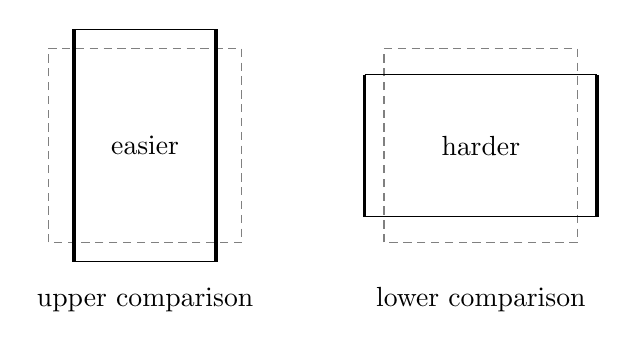
\begin{tikzpicture}[scale=.82]
 \begin{scope}
  \draw[densely dashed,gray] (0,0) rectangle (3,3);
  \draw (0.4,-.3) -- (2.6,-.3) (0.4,3.3) -- (2.6,3.3);
  \draw[very thick] (0.4,-.3) -- (0.4,3.3)
                   (2.6,-.3) -- (2.6,3.3);
  \node at (1.5,1.5) {easier};
  \node[below] at (1.5,-.55) {upper comparison};
 \end{scope}
 \begin{scope}[xshift=5.2cm]
  \draw[densely dashed,gray] (0,0) rectangle (3,3);
  \draw (-.3,.4) -- (3.3,.4) (-.3,2.6) -- (3.3,2.6);
  \draw[very thick] (-.3,.4) -- (-.3,2.6)
                   (3.3,.4) -- (3.3,2.6);
  \node at (1.5,1.5) {harder};
  \node[below] at (1.5,-.55) {lower comparison};
 \end{scope}
\end{tikzpicture}
\caption{The Jordan-quad comparison in Schoenflies coordinates.
The dashed square is the limiting target; thick sides are separately
wired electrodes.  The easier quad extends beyond the free sides and
ends inside the target's electrode sides.  The harder quad has the
opposite inclusions.  Physical test polygons retain strict margins
after pullback and lattice approximation.}
\label{jordan:sandwich-figure}
\end{figure}


For the upper bound, restrict both laws to their common primal edges
in the easier quad.  Any target edge outside this common graph can
attach to it only on its two electrode sides: the easier horizontal
sides lie strictly outside the target.  Outside pieces cannot join
the two electrode sides, even through a target wire block, because
the substantial intervening strip lies wholly inside the easier quad
and the two target wire blocks lie in separate exterior zones.
Thus the target's induced boundary partition on the common graph is
weaker than separate wiring of the easier electrodes.  Domain Markov
and FK monotonicity give a coupling in which the easier common-edge
configuration dominates the target's.  Every actual target crossing
contains a common-edge crossing of the easier electrodes.  Indeed,
follow it from the initial exterior zone to the opposite zone, taking
its last exit from the first and first entry into the second; its
intermediate edges must belong to the common graph.  There is no
escape through the distant horizontal sides.

For the lower bound interchange the roles using the harder quad.
Its exterior pieces can attach to the target only on the designated
target arcs, and cannot link opposite sides outside the common graph.
Here it matters that the target contains \emph{all} lattice edges in
its closure, and that both graphs use exactly the same primal grid.
The target wires therefore dominate the induced harder-quad
partition.  Every harder crossing contains an actual shared-edge
piece joining the two target arcs.  This proves the lower comparison.
All transitions occur at ordinary graph vertices; shrinking lattice
edges have uniformly shrinking diameter in Schoenflies coordinates,
so the strict margins justify the discrete versions of the statements.

The conformal cross-ratios of the two test quads tend to $\chi$.
Indeed uniformly convergent parametrizations of Jordan curves imply
uniform local connectedness of their boundaries: points close in the
image have parameters close in the circular order, except for the
identified endpoints, because the limiting parametrization is an
embedding.  Kernel convergence and boundary extension of normalized
Riemann maps then give marked conformal convergence
\citep{Pommerenke1992}; see also the explicit uniform-Jordan and kernel-convergence statements in \citet[Appendix~A, Theorems~6--8 and Corollaries~A.1--A.2]{CamiaNewman2006Convergence}.  Since $g$ is continuous on $(0,1)$, let first
$n\to\infty$ and then $\varepsilon\downarrow0$ in the two comparisons.
\end{proof}

\begin{corollary}[The prescribed bond-percolation crossing]\label{jordan:cardy}
At $q=1$, with every edge, including every boundary edge, sampled
independently with probability $1/2$ and with no wiring, the probability
of the event $C_n$ defined in Subsection~\ref{intro:crossings} tends to
\[
 \frac{\displaystyle\int_0^\chi [t(1-t)]^{-2/3}\,dt}
      {\displaystyle\int_0^1 [t(1-t)]^{-2/3}\,dt}.
\]
\end{corollary}
\begin{proof}
For $q=1$ the boundary partition does not change the edge law, and
$d=1$ gives $g=f$.  The $\rho=1/3$ specialization of the four-change
integral calculation is precisely the displayed expression.  The
comparison in Proposition~\ref{jordan:transfer} concerned actual edge
paths throughout, so no external wire is counted as a crossing and
no interface-event continuity assertion is needed.
\end{proof}

\section{Alternating tests after exploration}\label{sec:movingtests}

The Jordan result alone does not apply to a domain cut out by a random
exploration.  We prove the needed extension directly under the
original lattice law.  Conditional errors at exceptional histories
will be controlled by an \emph{averaged} six-arm estimate.

\subsection{Geometry and conditional laws}

We reveal a switch in full when the strand first encounters its tile,
then follow the prescribed local arc.  The revealing filtration records
these switch states and the current position on that arc.  A stopping
time for this filtration may therefore fall partway through an
already-revealed tile; it need not be a tile-completion time.  Below,
a \emph{switch-revealing stop} means any stopping time for this
filtration, including such a partial-tile stop.

\begin{lemma}[A compatible simple drawing]\label{moving:drawing}
The prescribed polygon graph and its Dobrushin strand admit a tile
and collar representation in a Jordan polygon $V_n$ such that:
\begin{enumerate}[label=(\roman*)]
\item $V_n$ has the same marked uniform Jordan limit as $D_n$;
\item the rounded strand is simple, visits the same ordered local
pieces as the prescribed medial strand, and is at curve distance
$O(\delta_n)$ from it;
\item at every stop for this revealing filtration, the remaining domain
is a simple slit disk.  Under deterministic cap closure its unrevealed edges have
the original conditional FK law, with known open edges contracted
and known closed edges deleted;
\item primal and dual banks of the prefix have physical access to
their corresponding known edges and wire vertices within
$O(\delta_n)$.  Every completion of the unknown edges embeds its
actual paths in the slit disk without crossing the past.
\end{enumerate}
The construction can use identical domains and caps away from an
interval where two additional boundary changes are inserted.
\end{lemma}

\begin{proof}
Make one tile for each edge of the polygon graph, including boundary
edges.  Glue the four triangles directed toward each interior square
center.  The exterior triangle of a boundary edge is a separate tab,
with its own outer dual vertex; do not glue different exterior tabs
along their radial sides.  Each primal boundary vertex retains all
its interior incidences.  Flatten the exterior tabs toward their
bases, to less than half their original height, and add a still
thinner Jordan collar.  The tabs are then disjoint except at their
prescribed vertices.  All changes lie within $O(\delta_n)$ of the
original boundary, and tracing the tabs and collar along the original
parametrization proves (i).

Draw the switches and boundary caps as disjoint arcs.  A local wire
can be drawn behind its cap in the collar.  The unmatched ports
continue to the marked outer-boundary points.  The finite choices
inside each tile and the collar can be made deterministically.
At a wired boundary edge, capping its outer dual vertex joins the
inside ports in the same way for either switch state.  Declaring that
edge open for the drawing merely substitutes a cap-sized detour and
possibly deletes a microscopic loop.  On the free side, the cap
around a primal vertex is exactly the turn beside the dual wired
arc.  Inside the polygon, glued half-segments give the specified
medial edges and their quarter-turn pairings.  Match corresponding
ordered pieces in the two drawings.  Each substituted piece lies in
boundedly many neighboring tiles, so simultaneous parametrizations
have distance $O(\delta_n)$.  Zero-length pieces are handled by limits
of increasing reparametrizations.  This also covers a midpoint visited
with both prescribed pairings and proves (ii).

The tile/cap Euler identity gives exactly the conditional FK law
asserted in (iii).  On a queried primal-open tile the adjacent primal
corners are joined by its actual edge; on a queried closed turn the
bank stays at one primal corner.  Along a cap it stays at one vertex
or uses neighbors already belonging to that wire interval.  Thus the
bank is a known chain attached to the appropriate original interval,
and every queried primal-open edge accesses this bank within one tile.
The same statement holds for dual edges.  Designated outer vertices
access their arcs through the collar.  These are physical accesses,
not additional identifications.  At a stop partway through a local arc,
the full state of its tile has already been revealed, and following
that known arc reveals no additional unknown edge.  The conditional
law in (iii) and these bank accesses in (iv) therefore apply at such
stops as well.  Projecting back to the usual primal
or dual lattice moves points by $O(\delta_n)$ and duplicates no edge;
separate virtual copies of a vertex may become one physical vertex.
\end{proof}

In a four-open-change experiment, deterministic closure with separate
wires of one color differs by a density depending only on the two
pairing outcomes.  This density and its reciprocal are bounded by
constants depending on $q$.  At a switch-revealing stopping time the
odds change is still exactly
\begin{equation}\label{moving:odds}
 p\longmapsto \frac{p}{p+d(1-p)}.
\end{equation}
One obtains this by conditioning the \emph{full} finite-sample density,
not by postulating a Markov property for a limiting curve.  Consequently
conditional rare-event probabilities in a deterministic-cap law can
be averaged under open-cap histories at a bounded multiplicative cost.

\begin{lemma}[Small-interval behavior]\label{moving:asymptotic}
For $f$ in \eqref{jordan:functions},
\[
 f(1-\chi)=1-f(\chi),\qquad
 f(\chi)=c_q\chi^h(1+o(1))\quad(\chi\downarrow0),
 \qquad c_q>0.
\]
\end{lemma}
\begin{proof}
The substitutions $u^{-1}$ in $I_C$ and
$u=1-(1-\chi)t$ in $I_B$, followed by the Euler transformation of
the beta integral, give
\[
 I_B(\chi)=\left(\frac{1-\chi}{\chi}\right)^h I_C(1-\chi).
\]
Both $I_C(0)$ and $I_C(1-)$ are finite and strictly positive: at the
possible singularity $u=1$, the latter integrand has exponent
$-2\rho>-1$, while the integrand at infinity has exponent
$-1-\rho<-1$.  Substitution into \eqref{jordan:functions} proves both
claims, with $c_q=I_C(0)/I_C(1-)$.
\end{proof}

\begin{theorem}[Moving four-change test]\label{moving:slit}
Let a four-change strand in $V_n$ be stopped before completing its
strand, revealing only the switches it has encountered.  Let $U_n$
be its remaining simple slit disk, with the tip as the new starting
mark.  Consider histories for which a fixed basepoint has a fixed
positive disk in $U_n$, and the four prime-end marks in a disk chart
normalized at that basepoint remain mutually separated by a fixed
positive amount.  Then, on these histories,
\begin{equation}\label{moving:limit}
 \mathbb P_{\mathrm{open}}(E_{\mathrm P}\mid\mathcal F_n)
       -f(\chi_{U_n})\ \longrightarrow\ 0
 \quad\hbox{in probability}.
\end{equation}
Here $E_{\mathrm P}$ is the primal pairing event, equivalently the
actual bridge event after separate primal closure, and $\chi_{U_n}$
is its current ordered cross-ratio.  The assertion holds for arbitrary
mesh-dependent stopping rules satisfying this localization.
\end{theorem}

For the comparison, first use separate deterministic primal closure
and let $u_n$ be the rectangle abscissa in $U_n$, with the two primal
electrodes at $0$ and $1$.  A \emph{possible primal path} is an
edge path after all still unknown primal edges have been filled open,
without using a wire identification as an edge.  We need the comparison
boundary to avoid vertices in the central part of $0<u_n<1$ that have
such a possible path to an electrode: every central vertex of an actual
crossing is among them.

We construct its boundary by routing a finite polygonal obstacle near
the explored bank.  Outside small protection balls and grid cells where
the past already supplies four alternating arms, the obstacle has
positive clearance from those vertices.  The exceptional
regions have small conditional attachment cost outside a set of
histories of small probability.  Rounding the obstacle gives a Jordan
domain $H$, selected from a finite list at each fixed accuracy.  There
is no inclusion requirement between $H$ and $U_n$.  Instead, matched
rectangle fibers align their abscissas along electrode paths that
avoid the exceptional regions.  After deleting the small-cost
exceptional edges, an original
crossing must contain a crossing of a trimmed test quad in $H$ on
their common graph, where the test wiring dominates the original
induced partition.  This gives the upper bound; exchanging colors
gives the other bound.

Every annulus used below lies
a fixed positive distance inside the original domain before its mesh
limit is taken.  The inputs are the bulk passage estimate of
Section~\ref{sec:preliminaries}, the vanishing full-lattice one-arm
bound with wired rims, and the six-arm estimate
\begin{equation}\label{moving:sixarm}
 \mathbb P(A_6(r,R))\le C(r/R)^{2+c_0},\qquad c_0>0,
\end{equation}
where $A_6(r,R)$ is the event of six cyclically alternating actual
primal-open and dual-open arms across the annulus.  The estimate holds
for the critical square-lattice FK law with this fixed $q<4$
\cite[Corollary~6.7]{DMT2021Fractal}.  An outer buffer and the bulk
boundary-condition comparison of Lemma~\ref{prelim:collar} transfer
this estimate from the infinite-plane law to the original finite law,
with the outer scale fixed.  Bounded open-cap
reweightings are harmless.  No six-arm estimate conditioned on an
arbitrary explored maze is asserted.

\begin{lemma}[Physical paths and chart oscillation]\label{moving:chart-modulus}
Let $u_n$ be the rectangle abscissa just defined.
Under the localization in Theorem~\ref{moving:slit}, there is a common
modulus tending to zero for the oscillation of $u_n$ on a connected
path of vanishing physical diameter, including paths with accesses
to the prime boundary.  Consequently, for $\beta>0$, a possible
primal path starting in $\beta\le u_n\le1-\beta$ cannot reach a known
primal-open edge or a primal electrode inside a sufficiently small
physical ball.
\end{lemma}
\begin{proof}
Away from the normalizing point, a connected set in a ball of radius
$r$ is hit before domain exit by Brownian motion from that point
with probability tending uniformly to zero as $r\downarrow0$.
Comparison with a fixed enclosing Euclidean annulus gives this
bound.  In the normalized disk, a connected set of a fixed positive
diameter has hitting probability bounded below; this follows, for
example, by a crosscut between separated angular sectors and the
Beurling estimate.  The rectangle maps of the disk form a compact
family because the four marks remain separated.  Thus a small
physical continuum cannot have a macroscopic rectangle-coordinate
oscillation.  Near the basepoint use interior distortion instead.
Endpoint accesses follow by interior approximation.

By Lemma~\ref{moving:drawing}, every known primal-open edge and fixed
primal wire attachment accesses $u_n=0$ or $1$ within
$O(\delta_n)$.  A short possible connection from the central band to
one of them would contradict the just-proved modulus.  Small buffers
in the band absorb individual tile errors.  In particular the two
opposite designated intervals have not already met through the
revealed bank under the stated nondegeneracy.
\end{proof}

\begin{lemma}[Deletion and protected-ball costs]\label{moving:deletion}
Fix a history and use separate deterministic primal closure.
Deleting a set of still random edges changes the actual crossing
probability by at most the probability, in the undeleted conditional
law, that an endpoint of a deleted edge reaches either wire interval
or its revealed primal bank by an actual open path, allowing one
initial test step over the deleted edge.  Contact at a wire vertex
may have length zero.
For a central-band set contained in a ball of radius $r$, this cost
is bounded by a quantity tending to zero as $r\downarrow0$,
uniformly in the history and center, provided its required outer
radius is fixed and the mesh is sufficiently small.  The same holds
for any fixed finite number of such balls.
\end{lemma}
\begin{proof}
The separate wire intervals and their revealed banks are the only
nontrivial identification blocks, by Lemma~\ref{moving:drawing}.
Couple the deleted and original laws monotonically.  Explore the
actual open clusters from all deletion endpoints in the stronger
configuration, revealing the corresponding edges in both laws.
FK partition monotonicity persists at every step.  After the clusters
are enclosed by their closed cuts, the conditional laws outside
agree and can be coupled identically.  If no explored cluster reaches
a wire interval, the crossing decision is unchanged.  This proves
the first assertion, including contact with a wire along a known bank.

Choose the fixed outer radius small enough for
Lemma~\ref{moving:chart-modulus}.  Every component of possible edges
inside this ball that meets the central-band set has no accessible
wire or known primal-open attachment.  Its uncertain boundary
connections can occur only at the ball rim.  Project to the physical
lattice, fill missing edges, and wire that rim.  Splitting physical
vertex copies only weakens the original induced partition.  The
full-lattice wired-rim law therefore dominates every relevant actual
arm simultaneously.  Cropping the ball slightly absorbs tile errors.
Its one-arm probability from radius $r$ to the fixed outer radius
tends to zero: buffered dual circuits from RSW block such an arm.
A finite union bound gives the last assertion.
\end{proof}

\subsection{A directed obstacle away from possible connections}

Fix a small trimming parameter $a_*>0$ and then
$0<\beta<a_*/20$.  A primal vertex is a \emph{candidate} if its chart
coordinate lies in $[\beta,1-\beta]$ and it has a possible connection
to an electrode.  Each candidate supplies a possible arm to a fixed
positive physical distance, by Lemma~\ref{moving:chart-modulus}.

\begin{lemma}[Flagged cells and their cost]\label{moving:flags}
In a fixed bulk block let $\pi$ be a simple known primal bank path.
Choose fixed scales $\ell\ll R_1$, away from its endpoints and the
original boundary.  Flag a deterministic grid cell of side $\ell$
if, in its annulus from $100\ell$ to $R_1$, the prefix already supplies
four cyclically alternating actual arms, its two primal arms being
known wired bank paths.  If a candidate within $O(\ell)$ of this cell
actually connects to an electrode, then six actual alternating arms
occur in a cropped annulus from $200\ell$ to $R_1/2$.
For a bounded region covered by the deterministic cells, the averaged
conditional attachment cost of all flagged cells is at most
\begin{equation}\label{moving:flag-sum}
 C\ell^{-2}(\ell/R_1)^{2+c_0}=O_{R_1}(\ell^{c_0}).
\end{equation}
The statement remains valid with one initial test step and with the
bounded cap changes in \eqref{moving:odds}.
\end{lemma}
\begin{proof}
The extra actual primal arm cannot make a lateral connection to
either known primal leg inside the wider annulus, even in the
all-unknown-primal-open completion, by
Lemma~\ref{moving:chart-modulus}.  On the side containing the extra
arm it is bracketed by the two known primal legs.  A planar crossing
alternative in each intervening strip supplies a dual radial
separator.  The original dual separator on the other side remains.
After cropping at both rims, these three primal and three dual arms
are disjoint and alternate.

For precision, thicken actual paths to their tile color territories.
An open transversal between two primal territories would give an
actual lateral bridge, with an error of at most one tile.  Its absence
forces a dual territorial radial crossing in the intervening
topological rectangle, which shadows a dual edge path in the cropped
annulus.  If the no-bridge test is made after every unknown primal
edge is opened, every dual separator so obtained consists of known
closed tiles.  Thus the four old legs and the separators used in
this argument are actual original edges; no auxiliary boundary
condition manufactures them.

Apply \eqref{moving:sixarm} in the original full-sample law to each
cell of the deterministic grid, then sum over $O(\ell^{-2})$ cells.
The center may have been selected by the past because the sum was
taken over the entire deterministic grid.  Bounded cap densities
control the averaged conditional probabilities under either history
law.  Markov's inequality now makes the conditional flagged-cell
cost small outside a set of histories of small probability.  This
is an annealed-to-conditional argument, with $R_1$ and all comparison
constants fixed before $\ell\downarrow0$.
\end{proof}

\begin{lemma}[Directed obstacle]\label{moving:obstacle}
After removing histories of arbitrarily small probability and allowing
an arbitrarily small conditional deletion cost, there is a Jordan
polygon $H$ containing the basepoint, selected from a finite list at
each fixed accuracy, with the following properties.
Its boundary follows the original boundary and explored prefix to
that accuracy; away from finitely many protected balls and flagged
cells it has fixed positive clearance from all central candidates.
As the accuracies decrease, $H$ and $U_n$ have the same pointed kernel
limits.  Artificial marks in $H$ may be chosen with disk angles
arbitrarily close to the corresponding angles in $U_n$.
\end{lemma}
\begin{proof}
We construct the obstacle in three stages, keeping the scale choices
in the order in which they are used.

\paragraph{Retained bank blocks.}
Retain only prefix
excursions reaching depth $r$ from the limiting Jordan boundary,
including each complete segment between successive visits to depth
$h_b\ll r$ and the last incomplete segment if present.  Their number
is tight, uniformly in small $h_b$, because each visits one of a fixed
finite family of bulk annuli at depth $r/2$.  First bound this number,
then choose $h_b$ small.  Join their boundary-near endpoints to the
exterior of a slightly larger polygon through protected balls of
radius $O(h_b)$.  Lemma~\ref{moving:deletion} controls central
attachments in these finitely many balls.  No boundary arm exponent
for the rough Jordan curve is needed.

Break the retained excursions into blocks of diameter at most
$\epsilon\ll h_b$, each contained with margin in a bulk square $S$
of side $10\epsilon$.  Successive displacement thresholds and the
bulk passage estimate make the number of blocks tight.  After fixing
a block-count cutoff, snap its endpoints to a much finer deterministic
grid and protect them by balls of radius $e\ll\epsilon$.  The actual
known primal bank gives a path between the true endpoints in $S$;
loop erasure gives a simple path $\pi$, possibly trivial.  Take
\[
 \ell\ll R_1\ll e,
\]
so all flag annuli are bulk annuli.

\paragraph{A connector avoiding possible attachments.}
Declare forbidden every closed
$\ell$-cell within $3\ell$ of a candidate, except flagged cells and
cells in enlarged endpoint protections.

There is a connector between the protected endpoints avoiding all
forbidden cells.  Otherwise planar cell separation gives a polygonal
circuit through a chain of touching forbidden cells and possibly the
exterior of $S$, separating the two endpoints.  It can be chosen
away from their protection balls and within a cell-sized error of
the cell chain.  Choose a candidate witness in each cell.  Two
successive witnesses can be joined avoiding $\pi$ inside a disk of
radius $O(R_1)$.  If they could not, a proper crosscut of the simple
path $\pi$ would separate them in a circle of radius between
$4R_1$ and $6R_1$.  Its full-path endpoints lie outside because the
cell is away from endpoint protections.  The crosscut passes within
$O(\ell)$ of the witness segment.  The two witnesses have possible
arms to that circle, on opposite sides of $\pi$, and cannot connect
locally to $\pi$ by Lemma~\ref{moving:chart-modulus}.  The two known
radial legs of $\pi$ and the two possible arms consequently interlace.
In each intervening strip the optimistic no-bridge test supplies a
\emph{known} dual radial separator, as in the proof of
Lemma~\ref{moving:flags}.  The cell is therefore flagged, a
contradiction.

Push the separating circuit through the witness points and these
avoiding joins.  Its displacement is $O(R_1)$, smaller than its
distance from the endpoints, so its winding distinction is preserved.
Along the exterior of $S$ avoidance is automatic because $\pi$ has
an interior margin.  We have obtained a separating circuit disjoint
from $\pi$, which is impossible.  Overlapping endpoint protections
or a trivial $\pi$ are handled by a connector within their union.

\paragraph{The exterior-attached obstacle and its kernel.}
Select one polygonal connector for each allowed finite grid pattern.
Their union and the protected exterior attachments form an obstacle
$K$ attached to the complement of the larger polygon.  The connectors
need not form one simple curve.  They stay close to the retained
prefix, and every omitted prefix piece is boundary-near; conversely
the entire prefix is approached by this obstacle or the outer wall.
Within distance $\ell/2$ of $K$, candidates occur only in flagged or
protected error regions.  The basepoint component of the complement
is simply connected, because each obstacle component is attached to
the exterior.  It is a fixed polygonal domain, possibly with slits
and pinches.  An interior radial approximation in its Riemann map,
followed by a polygonal perturbation, gives a Jordan domain $H$ whose
boundary is within $\ell/10$ of the obstacle or outer wall.
The outer wall was chosen much farther than $\ell$ from the original
graph.  Hence the asserted clearance holds.  Every choice is from a
finite list at fixed scales and count cutoffs.

Normalize maps of $H$ and $U_n$ at the same basepoint, and transfer
marks by finite-grid approximations to their disk angles.  On a
Hausdorff subsequence of the original boundary and prefix, every
compact path in the limiting basepoint component eventually belongs
to both constructions, while every limiting boundary point is
approached by complements of both.  Thus their pointed kernels agree,
and their normalized interior charts have the same limit.  This is
an interior statement; no locally connected boundary for the
limiting slit domain is asserted.  The fixed basepoint margin and
separation of the marks persist throughout.
\end{proof}

The obstacle and the comparison fibers have different jobs: the first
keeps the new boundary away from possible crossing attachments, whereas
the second aligns the two chart coordinates.  Figure~\ref{moving:comparison-figure}
illustrates these two geometric steps.

\begin{figure}[tb]
\centering
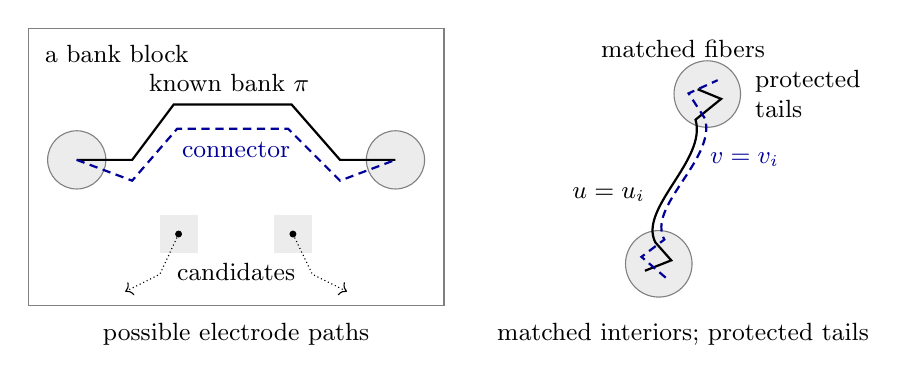
\begin{tikzpicture}[scale=.88,font=\small]
 \begin{scope}
  \draw[gray] (0,0) rectangle (6,4);
  \node[anchor=north west] at (.1,3.9) {a bank block};
  \fill[gray!15] (.7,2.1) circle (.42);
  \fill[gray!15] (5.3,2.1) circle (.42);
  \draw[gray] (.7,2.1) circle (.42) (5.3,2.1) circle (.42);
  \draw[thick] (.7,2.1) -- (1.5,2.1) -- (2.1,2.9)
    -- (3.8,2.9) -- (4.5,2.1) -- (5.3,2.1);
  \node[above] at (2.9,2.95) {known bank $\pi$};
  \draw[blue!60!black,thick,densely dashed]
    (.7,2.1) -- (1.5,1.8) -- (2.15,2.55)
    -- (3.75,2.55) -- (4.5,1.8) -- (5.3,2.1);
  \node[blue!60!black] at (3,2.25) {connector};
  \fill[gray!15] (1.9,.75) rectangle (2.45,1.3);
  \fill[gray!15] (3.55,.75) rectangle (4.1,1.3);
  \fill (2.17,1.03) circle (.05) (3.82,1.03) circle (.05);
  \draw[->,densely dotted] (2.17,1.03) -- (1.9,.45) -- (1.4,.2);
  \draw[->,densely dotted] (3.82,1.03) -- (4.1,.45) -- (4.6,.2);
  \node at (3,.48) {candidates};
  \node[below,align=center] at (3,-.12)
    {possible electrode paths};
 \end{scope}
 \begin{scope}[xshift=7cm]
  \node at (2.45,3.7) {matched fibers};
  \fill[gray!15] (2.1,.6) circle (.48);
  \fill[gray!15] (2.8,3.05) circle (.48);
  \draw[gray] (2.1,.6) circle (.48) (2.8,3.05) circle (.48);
  \draw[thick] (1.9,.5) -- (2.28,.65) -- (2.05,.91)
    .. controls (1.8,1.4) and (2.8,2.1) .. (2.63,2.68)
    -- (3,2.98) -- (2.66,3.12);
  \draw[blue!60!black,thick,densely dashed]
    (2.2,.4) -- (1.85,.7) -- (2.18,.95)
    .. controls (1.92,1.43) and (2.92,2.1) .. (2.77,2.69)
    -- (2.53,3.06) -- (2.95,3.25);
  \node[left] at (2.04,1.6) {$u=u_i$};
  \node[right,blue!60!black] at (2.7,2.1) {$v=v_i$};
  \node[right,align=left] at (3.35,3.05) {protected\\tails};
  \node[below,align=center] at (2.45,-.12)
    {matched interiors; protected tails};
 \end{scope}
\end{tikzpicture}
\caption{The two comparisons in the moving-domain argument, schematically.
Left: a deterministic connector stays near a retained known bank block
while avoiding central candidate neighborhoods; the dots have merely
possible electrode paths, not known open paths or bridges to the bank.
The endpoint balls are charged by the deletion estimate.  Flagged cells,
where an attachment is instead charged by the six-arm estimate, are not
shown.  Right: fibers of the rectangle abscissas $u$ in $U_n$ and $v$ in
$H$ match on compact interior portions; length--area confines their
remaining tails to common small balls.  Neither panel asserts that $H$
and $U_n$ are nested or that their slit boundaries converge uniformly.}
\label{moving:comparison-figure}
\end{figure}


\subsection{Alignment of the comparison charts}

\begin{proof}[Proof of Theorem~\ref{moving:slit}]
It suffices to prove an upper bound for the primal connection under
separate deterministic primal closure.  Interchanging the colors
and using the other deterministic closure gives the complementary
upper bound; \eqref{moving:odds} then yields the open-cap limit.

Use Lemma~\ref{moving:obstacle}, and write $u$ and $v$ for the rectangle
abscissas in $U_n$ and $H$.  Test on the Jordan subquad of $H$ between
$v=a_*$ and $v=1-a_*$, with these sides separately wired.  At fixed
accuracy there are finitely many such quads; approximate each on the
original color grid by the polygon construction of
Proposition~\ref{jordan:transfer}.  Their limiting crossing
probabilities differ from $g(\chi_{U_n})$ by arbitrarily small
trimming, chart-angle, and kernel errors, uniformly under the
nondegeneracy assumptions.

\paragraph{Matched fibers and their protected tails.}
To align the charts along crossing paths, take a fine finite grid of
abscissa bins in the central part of $(0,1)$, with width much smaller
than both $\beta$ and $a_*$.  In each bin choose a nearby vertical
fiber for each chart.  Its central part is a compact internal curve
and is matched in the other chart by kernel convergence.  Its two
remaining tails can be confined to balls of vanishing radius,
with matched centers.  Here is the required length--area argument.
Remove small fractions of rectangle height at top and bottom.
For each fixed fraction, inverse maps and derivatives converge on
the compact retained rectangles.  Let that fraction decrease slowly.
For a bin $I$ and a deleted height interval $J$, Cauchy--Schwarz gives
\[
 \int_I\!\operatorname{length}\bigl(\Phi(\{x\}\times J)\bigr)\,dx
 \le (|I||J|)^{1/2}
       \left(\int_{I\times J}|\Phi'(z)|^2\,dA(z)\right)^{1/2},
\]
where $\Phi$ is the inverse rectangle map.  The last integral is
bounded by the common physical area bound.  Choose levels in each
bin controlling the tails of both charts.  Their initial endpoints
match on the retained compact pieces, so matched small endpoint
balls contain all four tails.  This argument does not require
uniform local connectedness of the explored boundaries.  Tile errors
are absorbed by decreasing the fractions slowly enough.
Lemma~\ref{moving:deletion} controls the conditional attachment cost
of these finitely many endpoint balls.

\paragraph{Deleting edges that obstruct comparison.}
Delete still unknown edges touching a slightly narrower band,
initially $3\beta\le u\le1-3\beta$, if their endpoints fail containment
in $H$ with a sufficiently small fixed fraction of the clearance
$\ell$, or if their two abscissas differ by more than $a_*/10$.
These deletions have negligible conditional crossing cost.  To see
this, suppose an endpoint of such an edge reaches an electrode by
an actual path, allowing the initial test step.  Paths meeting a
flagged cell, protection ball, or fiber-endpoint ball while centrally
located already have negligible total cost.  For every other path,
trace it inward from the electrode after its last entry into the
broader band $2\beta\le u\le1-2\beta$.  It crosses a comparison
$u$-fiber on its main internal piece, giving an anchor in $H$ with
nearly equal abscissas.  It cannot subsequently leave $H$, since its
central vertices are candidates and the wall has clearance from
them.  Each later crossing of either chart's comparison fiber is
again on its main piece.  If $v$ drifted by more than a few bin
widths from $u$, it would cross a $v$-fiber in a nonmatching $u$-bin,
a contradiction.  The endpoint therefore has neither proposed
defect.  Vertices without a possible electrode connection can be
discarded at no crossing cost.  Smaller nested bands and clearance
constants accommodate complete edge segments and physical-grid
projection.

\paragraph{The induced partition on the common graph.}
Now keep the surviving uncertain edges in
$4\beta\le u\le1-4\beta$ that also belong to the trimmed test graph.
A nonshared original piece can attach to these only on a designated
side of the test quad: clearance excludes its free horizontal sides,
and the abscissa buffers exclude an attachment from a noncentral
piece.  No nonshared piece, even with history wires, connects the
two designated sides.  Such a traversal must pass through the middle
shared strip by chart matching, while all identifications lie in the
two separate groups near $u=0,1$.  After matching physical vertices,
the induced original partition is thus dominated by the test law's
separate wiring.  Every modified original actual crossing contains
a shared crossing between the test sides, by taking its traversal
from the first exterior group to the second.  Domain Markov and
partition monotonicity give the desired test upper bound.

\paragraph{Order of the approximations.}
The construction has the following quantifiers.
If convergence in probability failed with fixed error and probability,
choose first $a_*$ small, then $\beta$ and fiber precision smaller.
Choose obstacle accuracies tending to zero, with, at each stage,
a deep-excursion cutoff, boundary protection radius $h_b$, block
sizes and count cutoffs, endpoint protections $e$, the intermediate
radius $R_1$, and finally the flag scale $\ell$.  The conditional
protection costs and the averaged flag cost
\eqref{moving:flag-sum} are made small in that order.  For each fixed
stage choose the lattice mesh small enough for every geometric margin
and each of the finitely many Jordan test limits.  Select failing
histories outside all exceptional sets, and pass to a common kernel
subsequence.  The fiber argument and additional deletions along this
subsequence have uniform conditional error by
Lemma~\ref{moving:deletion}, and contradict the failure.  All six-arm
summations took place under the original law before this deterministic
selection of histories.  This proves \eqref{moving:limit}.
\end{proof}

\section{Identification of the Dobrushin strand}\label{sec:chordal}

The moving four-change tests first determine the limiting Loewner
driver.  We then combine that identification with physical compactness
and crossing estimates to identify the entire ordered Dobrushin curve.

\subsection{Two small tests determine the driver}

Map $V_n$ to $\mathbb H$, sending its two Dobrushin ends to $0$ and
$\infty$, with a convergent interior normalization.  The inverse maps
converge uniformly in disk coordinates, including the boundary, by
marked Jordan convergence.  Choose the orientation so that the
positive real side is primal-free.  The rounded simple strand has a
continuous Loewner driver $W_t^{(n)}$, with
\begin{equation}\label{chordal:loewner}
 \partial_t g_t^{(n)}(z)=\frac{2}{g_t^{(n)}(z)-W_t^{(n)}},
 \qquad g_0^{(n)}(z)=z,\qquad W_0^{(n)}=0.
\end{equation}
We suppress the superscript when discussing a single mesh.
Fix $T,R<\infty$ and stop at $T$ or the first exit of $|W_t|<R$.
All constants in this subsection may depend on these fixed bounds.

\begin{lemma}[Bounded martingale tests]\label{chordal:tests}
For every $x>2R+1$, put
\begin{equation}\label{chordal:martingale}
 M_t(x)=\left(\frac{xg_t'(x)}{g_t(x)-W_t}\right)^h.
\end{equation}
These processes and their reciprocals are bounded on the stopped
range, uniformly in the mesh.  For arbitrary stopping rules
$0\le\sigma_n\le\tau_n$ in that range and uniformly bounded
$\mathcal F_{\sigma_n}$-measurable tests $F_n$,
\begin{equation}\label{chordal:approx-martingale}
 \mathbb E\!\left[F_n\bigl(M_{\tau_n}(x)-M_{\sigma_n}(x)\bigr)\right]
 \longrightarrow0
\end{equation}
under the original single-strand Dobrushin law.
\end{lemma}
\begin{proof}
Insert on the original free side a small separate primal interval
whose endpoints in the initial coordinate approximate $x,x+s$.
Use the four-open-change experiment.  Until the specified stop its
cross-ratio is
\[
 \chi_t=\frac{g_t(x+s)-g_t(x)}{g_t(x+s)-W_t}.
\]
The real Loewner solutions remain separated from the driver and
from one another.  At each fixed $s>0$ the four marks, including
$\infty$, therefore stay nondegenerate.  A physical point corresponding
to $iM$ for sufficiently large fixed $M$ has a fixed unaffected disk;
it supplies the basepoint in Theorem~\ref{moving:slit}.  The trajectory
cannot end at either inserted mark within this localization.

Let $Z_t$ be the conditional pairing probability.  It is an exact
bounded martingale.  At any of the allowed stopping rules,
Theorem~\ref{moving:slit} gives $Z_t-f(\chi_t)\to0$ in probability,
and hence in mean, for fixed $s$.  Divide the martingale identity by
$f(s/(x+s))$ only at this fixed $s$.  Lemma~\ref{moving:asymptotic}
and analytic ODE estimates near $x$ give, uniformly in the stopped
range,
\begin{equation}\label{chordal:small-test}
 \frac{f(\chi_t)}{f(s/(x+s))}
     =\left(\frac{xg_t'(x)}{g_t(x)-W_t}\right)^h+o_s(1),
\end{equation}
after the mesh limit.  The expression on the right is bounded above
and away from zero independently of small $s$:
$g_t(x)-W_t$ is bounded below, $g_t(x)$ is bounded above, and
\[
 g_t'(x)=\exp\left(-\int_0^t\frac{2\,du}{(g_u(x)-W_u)^2}\right)
\]
has the same bounds.

We next compare the laws, after replacing the normalized conditional
probabilities by the bounded expressions in
\eqref{chordal:small-test}.  Separate deterministic four-change
closure adds just the small wire interval to the Dobrushin law.
Couple monotonically and explore clusters from that interval in the
stronger law.  The probability that its actual cluster reaches a
fixed small outer neighborhood tends to zero as the interval shrinks.
Inside the intervening annulus there are no wire attachments away
from the rims, since the old primal wire is a positive distance away.
Filling to the full-lattice wired-rim law dominates the arm, which
is blocked by the buffered RSW circuits.  Outside this neighborhood
the configurations can consequently be coupled identically.
The open-four and deterministic-four laws also have vanishing total
variation difference: their density depends only on the pairing,
and the exceptional pairing has probability
$g(s/(x+s))\to0$.  The stopped strands stay outside a fixed
neighborhood of the insertion point, by the separated real and
nearby complex solutions of \eqref{chordal:loewner}.  The drawing and
caps were chosen identical off that neighborhood.

Thus bounded stopped-history functions of $M$ transfer with vanishing
error, first as the mesh tends to zero and then as $s\downarrow0$.
We never divide a coupling error by $f(s/(x+s))$.  The same stopping
rules are applied in the coupled experiments, so the conclusion
includes mesh-dependent rules and yields
\eqref{chordal:approx-martingale}.
\end{proof}

\begin{proposition}[Driving convergence]\label{chordal:driver}
On every compact capacity interval, the Dobrushin driving functions
converge in law, uniformly, to $\sqrt\kappa B_t$, where $B$ is standard
Brownian motion and
\begin{equation}\label{chordal:kappa}
 \kappa=\frac{8}{1+h}
        =\frac{4\pi}{\arccos(-\sqrt q/2)}.
\end{equation}
\end{proposition}

\begin{proof}
We first work inside the preceding localization.  Set
\[
 X_t(x)=g_t(x),\qquad A_t(x)=x^h g_t'(x)^h,
 \qquad M_t(x)=A_t(x)(X_t(x)-W_t)^{-h}.
\]
The processes $X,A$ are uniformly bounded and uniformly Lipschitz
in time there, with $A$ bounded away from zero.  Take
$2R+1<x_1<x_2$.  Their real solutions stay separated: their gap
solves
\[
 \partial_t(X_t(x_2)-X_t(x_1))
 =-\frac{2(X_t(x_2)-X_t(x_1))}
 {(X_t(x_1)-W_t)(X_t(x_2)-W_t)}.
\]
It consequently has a positive lower bound on the stopped range.

Here is the two-test convexity argument in detail.
At a stopping time $\sigma$, freeze $X,A$ and write
$F_j(w)=A_\sigma(x_j)(X_\sigma(x_j)-w)^{-h}$.
Both derivatives are positive, and
\[
 \frac{F_1'(w)}{F_2'(w)}
 =\frac{A_\sigma(x_1)}{A_\sigma(x_2)}
   \left(\frac{X_\sigma(x_2)-w}{X_\sigma(x_1)-w}\right)^{h+1}
\]
has derivative uniformly bounded below by a positive constant on
$[-R,R]$.  Thus for
$a_\sigma=F_1'(W_\sigma)/F_2'(W_\sigma)$, a bounded predictable
quantity, integration of the derivative difference on either side
of $W_\sigma$ gives
\begin{equation}\label{chordal:two-test}
 F_1(w)-F_1(W_\sigma)
 -a_\sigma\bigl(F_2(w)-F_2(W_\sigma)\bigr)
 \ge c(w-W_\sigma)^2.
\end{equation}
The change of the frozen $X,A$ between $\sigma$ and $\tau$ costs at
most $C(\tau-\sigma)$.  Applying
\eqref{chordal:approx-martingale} to these two increments, with the
predictable coefficient incorporated into the test, yields
\begin{equation}\label{chordal:increment}
 \mathbb E[(W_\tau-W_\sigma)^2]
 \le C\mathbb E[\tau-\sigma]+o(1)
\end{equation}
for every sequence of allowed stopping rules.  Boundedness and
\eqref{chordal:increment} give the stopping-time tightness criterion
in the Skorokhod $J_1$ topology.  Since every path is continuous,
all subsequential limits are continuous, and the convergence may
be realized uniformly on compact stopped time intervals.

At inner localization levels chosen to be continuity levels of the
hitting operation, ODE continuity and
\eqref{chordal:approx-martingale} make each $M(x)$ a martingale in
the limit.  Such levels can increase to any outer localization.
The identity
\[
 W_t=X_t(x)-\left(A_t(x)/M_t(x)\right)^{1/h}
\]
and the positive bounds on $A,M$ show that $W$ is a continuous
semimartingale.  Write its decomposition as a local martingale plus
a continuous finite-variation process $B^{\mathrm{fv}}$, and let
$[W]$ be its quadratic variation.  With $Z=X-W$,
\[
 dX=2Z^{-1}\,dt,\qquad d\log A=-2hZ^{-2}\,dt.
\]
It\^o's formula gives the finite-variation part of $dM/M$ as
\[
 hZ^{-1}\,dB^{\mathrm{fv}}-4hZ^{-2}\,dt
       +\frac{h(h+1)}2Z^{-2}\,d[W].
\]
Since $M$ is a martingale, multiplication by $Z^2/h$ yields the
identity of signed measures
\begin{equation}\label{chordal:characteristics}
 (X-W)\,dB^{\mathrm{fv}}-4\,dt
       +\frac{1+h}{2}\,d[W]=0.
\end{equation}
Subtract the identities for $x_1,x_2$.  Their positive separation
forces $dB^{\mathrm{fv}}=0$, and then
$d[W]=8(1+h)^{-1}dt$.  L\'evy's characterization identifies the
localized law as Brownian with the rate in \eqref{chordal:kappa}.
The trigonometric identity follows from
$\arccos(-d/2)=\pi-\lambda$.

Finally, the probability of exiting a large outer driver bound
before $T$ is bounded in the limit by the Brownian probability of
hitting inner bounds approaching it.  These probabilities tend to
zero as the bounds increase.  Remove localization to obtain full
compact-time driving convergence.  Every subsequential law has been
identified, so the convergence holds along the full mesh sequence.
\end{proof}

\subsection{Physical compactness and avoidable crossings}

The use of annular crossings to control random curves was developed
by \citet{AizenmanBurchard1999}; conditional avoidable-crossing criteria
for compatible curve and Loewner convergence were developed by
\citet{KemppainenSmirnov2017}.  We give the physical compactness and
traversal arguments needed for the present boundary conventions
explicitly below.

\begin{lemma}[Territorial arm counting]\label{chordal:territories}
In a buffered bulk annulus, $m$ disjoint radial medial sublegs force
at least $m$ alternating actual primal/dual arms in a further cropped
annulus.  If only one color is retained, one obtains at least one
crossing in a distinct intervening strip per two assignments of that
color to successive medial separators.
\end{lemma}
\begin{proof}
The rounded medial arcs divide tiles into primal and dual territories.
A path within a territory shadows a path of its color on the physical
lattice: within a tile it passes to the corresponding corner, and
passage between opposite corners uses precisely the edge supplied
by that switch.  The shadowing has an error bounded by one tile.
Actual paths stay inside their territories.

Take disjoint simple radial sublegs, perturbing both annular radii
within buffers to regular values.  Thin parallel crosscuts on their
two sides give ordered territorial crossings of opposite colors at
each separator.  Compress successive runs of equal color in the
cyclic list.  Each medial separator contributes a color transition,
so at least $m$ alternating crossings remain.  Shadow them by lattice
walks in the central crop.  Near the wider rims keep territorial tails
until they can be spliced to the walks; thus no positive mesh-width
clearance of the thin territorial paths at the rims is needed.
Opposite-color paths are disjoint.  Same-color members of the
alternating list lie in different strips separated by an
opposite-color territorial path and cannot meet.  Disjoint tails
from the inner wider rim preserve order at first hits of the outer
cropped rim; taking last passages to those hits gives the claimed
actual arms.  The same strip ordering, after ignoring the other
color's assignments, proves the last assertion.
\end{proof}

\begin{lemma}[Curve compactness and no triple visits]\label{chordal:compactness}
The physical Dobrushin strands are tight in the uniform Euclidean
curve topology modulo increasing reparametrization.  Every
subsequential limit has no nonconstant interval on the original
boundary, and no interior point is visited three times with
nonconstant excursions between consecutive visits.
\end{lemma}
\begin{proof}
Bulk passage counts in a fixed finite family of buffered annuli are
tight by Section~\ref{sec:preliminaries}.  We first show that a
macroscopic displacement confined to a shrinking neighborhood of the
original boundary has vanishing probability.  In fixed plane
Schoenflies coordinates for $D$, such a displacement crosses
longitudinally one of finitely many boundary subarcs of positive
length, after shortening the subpassage to avoid the two change
points.  On each subarc the boundary type is homogeneous.  Its
nonwired-color bank is an actual path using that color's edges.

Surround the subarc by a thin Jordan ribbon and place the permitted
path in a still thinner band with strict margins.  Fill to the full
lattice of the bank color and wire the ribbon's outer boundary.
This dominates the actual crossing: there is no nearby designated
wire of this color, and all exterior attachments to the shared graph
occur on its ordinary sides.  Longitudinal ribbon crossings become
unlikely as the ribbon narrows.  One concrete proof chooses any
number $N$ of ordered intermediate positions on the subarc, each
with its own disjoint fixed neighborhood.  At each position two
across-ribbon sections can be confined to arbitrarily small physical
balls.  A longitudinal crossing must then traverse a Euclidean
annulus of arbitrarily large logarithmic aspect ratio inside that
subribbon; its extremal length tends to infinity.  Choose transverse
blocker quads with bounded transverse extremal distance and with outer
margins beyond the permitted band.  The strong quad RSW theorem
\cite[Theorem~1.2]{DMT2021Fractal} gives an actual opposite-color
transverse blocker with conditional probability at least $c>0$,
under arbitrary exterior partitions.  Approximate the fixed Jordan
corridors by polygons with strict margins before taking the mesh
limit.  Successive conditioning over the disjoint quads bounds the
crossing probability by $(1-c)^N$.  Let $N$ grow and then narrow the
ribbon.  Every geometric scale here was fixed before the mesh limit.

At a fixed displacement accuracy, outside these unlikely boundary
travels, every excess collection of successive displacements forces
many passages through a finite annulus cover of the compact part
away from the ribbon.  The passage estimates therefore bound the
number of successive displacements at each accuracy.  Subdivide
curves at these displacement times and apply the usual
Arzel\`a--Ascoli argument modulo reparametrization.  This proves
tightness and also rules out a nonconstant interval of a limit
confined to the original boundary.

Three genuine visits to an interior point, with positive intervening
excursions, produce six disjoint medial legs to some fixed positive
outer radius.  Lemma~\ref{chordal:territories} turns them into six
alternating actual arms across a cropped annulus.  Cover the possible
contact points by a deterministic grid of mesh $\ell$.  The bulk
six-arm estimate and the $O(\ell^{-2})$ grid count give a bound
$O(\ell^{c_0})$.  First take the lattice mesh limit, then
$\ell\downarrow0$, and finally a countable union over interior
compact sets and rational excursion radii.  This excludes precisely
three visits separated by nonconstant excursions; constant waiting
intervals are irrelevant to the curve topology.
\end{proof}

\begin{lemma}[Macroscopic avoidability]\label{chordal:avoidability}
At a switch-revealing stop of the Dobrushin exploration, call a
component of $U_n\cap A(z;r,R)$ \emph{avoidable} if it does not
separate the tip access from the target access inside $U_n$.
The conditional probability of a future radial traversal in any
avoidable component is bounded by a quantity tending to zero as
$r/R\downarrow0$, uniformly over histories and centers, with $r,R$
fixed before the mesh limit and $\delta_n\ll r$.
\end{lemma}
\begin{proof}
An avoidable component cannot access both designated primal and
dual prime boundary arcs strictly between the rims.  A path joining
such accesses contains a crosscut separating the tip from the target.
The future simple strand traverses one component between rims;
choose a color whose designated boundary is absent there.  Its bank
supplies an actual arm of unqueried edges in a cropped annulus.
A known-open edge or wire jump of that color would give a short
physical access to its designated boundary there, contrary to the
choice of component.

To bound all such components at once, keep their random edges of
this color within a cropped grid annulus.  Unqueried tiles are uncut;
an adjacency of incident edges, or attachment to a known edge or
wire vertex, has a corresponding $O(\delta_n)$ path in $U_n$ until
it reaches a designated wire.  Thus away from the cropped rims the
induced partition contains only ordinary physical-vertex attachments.
Delete known edges of the opposite state, fill the rest to the full
lattice, and wire both rims.  FK monotonicity dominates all the
relevant actual arms simultaneously by one full-lattice arm event.
Buffered dual circuits give its vanishing bound.  Sum over the two
possible missing colors.  The argument uses the conditional FK law
at actual revealing stops; an optional last piece of length
$O(\delta_n)$ is absorbed by the buffers.
\end{proof}

\begin{corollary}[No return from a small target cap]\label{chordal:target}
After the strand first enters a shrinking initial conformal cap
around its target, the probability of a subsequent displacement of
fixed positive physical size tends to zero.
\end{corollary}
\begin{proof}
At the first entrance the previously untouched cap gives a route
from the tip to the target inside a small physical ball.  Stop just
before entrance, or at the entering piece and use its bank with a
one-step buffer.  Outside this inner ball every relevant annular
component is avoidable.  Apply Lemma~\ref{chordal:avoidability}.
The diameters of the initial conformal caps shrink uniformly because
the initial inverse disk maps converge uniformly up to the boundary.
\end{proof}

\subsection{The ordered trace, including zero-capacity intervals}

Driving convergence and physical compactness leave one traversal issue:
a limiting curve could still move during an interval on which its
half-plane capacity is constant.  The next two lemmas provide the
ingredients for excluding this extra motion.

\begin{lemma}[Interior double visits in every time interval]
\label{chordal:dense-doubles}
For ordinary chordal $\mathrm{SLE}_\kappa$, $4<\kappa<8$, almost surely
every nonempty open capacity interval contains both visits to some
interior self-double point.
\end{lemma}
\begin{proof}
The double-point and boundary-hit dimension theorems of Miller--Wu
\cite[Theorem~1.1 and Corollary~1.7]{MillerWu2017} give, respectively,
\[
 1+\frac\kappa8-\frac6\kappa
 \quad\hbox{and}\quad 2-\frac8\kappa.
\]
Their difference is $(\kappa-4)^2/(8\kappa)>0$, so the trace has
an interior double point almost surely.  Let $E_T$ mean that both
visits occur strictly before $T$.  Scaling makes $\mathbb P(E_T)$
independent of $T>0$, while $\bigcup_{m\ge1}E_m$ has probability one.
Thus $\mathbb P(E_T)=1$ for every $T>0$.  At a deterministic time $a$,
the domain Markov property restarts ordinary SLE with additive
capacity clock.  An interior double point of the restarted trace
maps under $g_a^{-1}$ to an interior point of the original remaining
domain.  Apply this observation to all rational open intervals.
\end{proof}

\begin{lemma}[Small gates exclude swallowed excursions]
\label{chordal:gates}
In a joint subsequential limit of the physical strand and its
Loewner driving function, the physical curve cannot enter an open
component of a Loewner hull that is disjoint from the Loewner trace
and the original boundary.
\end{lemma}
\begin{proof}
Use the continuous Brownian SLE trace
\cite{RohdeSchramm2005}; here $4<\kappa\le6$.  Suppose that the
claimed excursion occurs.  By a countable choice, there is a small
closed ball $J$ with a larger buffered neighborhood disjoint from
the SLE trace and original boundary, approached deeply inside a
swallowed component at finite limiting capacity.  Fix bounds for
this capacity and the driver, and a high basepoint corresponding
to $iM$ in the initial half-plane coordinate.  Take the first discrete
approach to an intermediate buffer around $J$, before the alleged
hit.  Along a subsequence of these approach times the prefix keeps
a fixed spare distance from $J$, whereas its kernel viewed from the
basepoint excludes $J$.  This follows from driving convergence and
equality of the accessible Loewner domains; the whole buffered ball,
being disjoint from the trace, lies in one excluded component.

Nevertheless $J$ is still internal in every discrete simple slit
disk.  Normalize its inverse disk map $\Phi_n$ at the basepoint and
write $z_n=\Phi_n^{-1}(\operatorname{center}J)$.  Kernel convergence
forces $|z_n|\to1$.  Put $\epsilon_n=1-|z_n|$, and take circular
disk crosscuts centered at $z_n/|z_n|$, with radii between
$2\epsilon_n$ and $\sqrt{\epsilon_n}$.  If $L_n(t)$ is their image
length, Cauchy--Schwarz and the area formula give
\begin{equation}\label{chordal:gate-area}
 \int_{2\epsilon_n}^{\sqrt{\epsilon_n}}
            L_n(t)^2\,\frac{dt}{t}
       \le2\pi\operatorname{area}(U_n).
\end{equation}
The right side is uniformly bounded and the logarithmic integration
range diverges, so one image crosscut has diameter tending to zero.
Its disk cap contains $z_n$, and its endpoints access the slit
boundary.  Since that boundary stays a fixed distance from $J$, the
crosscut separates all of $J$ from the basepoint for sufficiently
large $n$.

The target is on the basepoint side.  Indeed the driver and capacity
bounds give a fixed route high above the half-plane hulls from the
basepoint to the target, with positive physical separation from the
prefix.  A small gate touching the prefix misses this route.  A gate
with both endpoints on the original outer wall cannot separate two
fixed interior balls when its diameter tends to zero, by uniform
Jordan convergence.  Adding a boundary-to-interior simple slit
disjoint from that gate does not change its separation.  Gates with
an endpoint at the initial slit attachment are included among gates
touching the prefix.

We must use a stopping rule, not a gate selected from the future
excursion.  Fix a small $\ell>0$ and stop at the first discrete step
at which there exists a crosscut of diameter at most $\ell$
separating $J$ from both basepoint and target, while the prefix still
keeps the chosen spare distance from $J$ and the basepoint is safe.
The preceding construction shows that this stop occurs before the
offending buffered hit for fine meshes.  Choices can be fixed
measurably from each finite history.  At first occurrence a witnessing
gate has an endpoint on the latest microscopic step, including its
attachment point.  Otherwise it was a crosscut of the previous slit
domain with the same separation: adding a disjoint simple slit
cannot change that separation.  This contradicts first occurrence.
The tip therefore reaches the gate and its target-side bank within
a ball of radius $\ell+O(\delta_n)$.

Choose a fixed outer radius smaller than the spare distance to $J$.
In the annulus from $4\ell$ to this radius about the new gate
endpoint, components on the trapped side are avoidable: a
tip-to-target route crosses the gate inside the inner ball and stays
on its other side.  Any later hit of $J$ requires a radial traversal
on the trapped side, since every return through the gate is inside
the inner rim.  Lemma~\ref{chordal:avoidability}, applied at this
first-gate stop, makes its conditional probability vanish as
$\ell\downarrow0$ after the mesh limit.  There is no sum over possible
gate locations.  This contradicts the alleged excursion.
\end{proof}

\begin{theorem}[Dobrushin convergence for $1\le q<4$]
\label{chordal:trace}
For every bounded marked Jordan domain and every marked uniform
polygon approximation satisfying Equation~\eqref{intro:marked-jordan}
with the boundary conventions of Subsection~\ref{intro:model}, the Dobrushin
strand converges in law, in the uniform Euclidean oriented-curve
topology modulo increasing reparametrization, to chordal
$\mathrm{SLE}_{\kappa(q)}$.
\end{theorem}
\begin{proof}
By Proposition~\ref{chordal:driver} and
Lemma~\ref{chordal:compactness}, take a joint subsequence realized
with compact driving convergence and uniform physical curve
convergence up to reparametrization.  Write $Y(t)$ for the physical
Brownian SLE trace, and $\gamma(s)$ for the full limiting physical
curve in an arbitrary forward parametrization.  Before its first
target visit, let $c(s)$ be the half-plane capacity of the hull of
its initial segment.  Kernel convergence makes $c$ continuous and
nondecreasing and identifies it as the limit of the corresponding
discrete capacities.  These mapped segments are bounded locally
away from the target.  As the target is approached, $c(s)\to\infty$:
a driver bounded on every finite capacity interval has its finite-time
hulls in bounded portions of the initial half-plane.

The domain accessible toward the target after time $s$ is the
Loewner remaining domain of $Y$ at time $c(s)$, by kernel convergence
and the Loewner ODE.  On every interval where $c$ changes, the newly
added trace segments of $\gamma$ and $Y$ have a point in common:
a boundary point of the smaller shared remaining domain inside the
older domain belongs to both increments.  Continuity, with shrinking
such intervals, implies
\[
 \gamma(s)=Y(c(s))
\]
at every time outside the interiors of plateaus of $c$, including
their active endpoints.  A nonconstant plateau is therefore an extra
excursion based at $Y(t)$, with $t$ its constant capacity, contained
in the old closed hull or original boundary.

Lemma~\ref{chordal:gates} excludes motion inside an open swallowed
component.  Hence an extra plateau can move only on $Y([0,t])$ or
the original boundary.  By Lemma~\ref{chordal:compactness}, it has
no varying subinterval entirely on that boundary.  If the plateau
were nonconstant, choose a compact varying subinterval in its
interior whose image avoids both the boundary and its basepoint.
Every image point has a unique old SLE time: two old visits together
with this genuine extra visit would give three interior visits
separated by nonconstant excursions, forbidden by
Lemma~\ref{chordal:compactness}.  This old-time inverse is continuous.
Indeed any sequence of old times has a convergent subsequence in
$[0,t]$, and trace continuity and uniqueness identify its limit.
Composing with the extra subcurve yields a continuous nonconstant
real function, whose image contains a nonempty capacity interval.
Lemma~\ref{chordal:dense-doubles} provides a point in that interval
with two old visits, a contradiction.  Thus every plateau is
constant.  The same reasoning at capacity zero excludes an initial
extra motion.

Corollary~\ref{chordal:target} excludes further motion after the first
limit target visit.  The capacity change of time therefore identifies
the entire ordered curve with $Y$, up to the permitted increasing
reparametrizations and constant waiting intervals.  Finally
Lemma~\ref{moving:drawing} transfers this conclusion from the rounded
simple drawing to the specified medial strand at distance
$O(\delta_n)$, including repeated midpoint visits with fixed pairings.
All subsequential limits agree, proving the claimed full-sequence
convergence.
\end{proof}

\section{Peeling along monochromatic walls}
\label{sec:peeling}

Throughout Sections~\ref{sec:peeling}--\ref{sec:loops}, fix
$1\le q<4$ and write $4<\kappa=\kappa(q)\le6$.
We now construct a joint exploration toward interior targets.  The boundary
conditions in this construction are part of the proof: its initial law is
the wired FK law in a square, and its final application will be to the
free infinite-volume law of Subsection~\ref{intro:collections}.

\subsection{Actual walls, caps, and the exact exploration law}
\label{peel:construction}

Begin with a nearest-neighbor square whose boundary primal edges are
deterministically open.  Attach to the inward side of each boundary edge
the corresponding half-tile.  Its two ports are paired around its dual
corner; this triangle contains no random switch.  More generally, a
\emph{homogeneous wall} of color $C\in\{{\sf P},{\sf D}\}$ consists of
actual open $C$-edges and these deterministic triangles on its inward
side.  Actual paths along the wall are allowed.  This distinction from
an abstract boundary identification will be used in every crossing
argument below.

All strands are oriented with primal on the left.  To start an
exploration in a primal-walled component, remove one wall triangle.
Enter at its earlier port in counterclockwise boundary order; the other
port is the force port.  On a dual wall reverse the boundary order.  The
boundary of an active component, in counterclockwise order, is
\begin{equation}\label{peel:boundary}
 P_WD_W,\qquad [D_W,D_O]_{\sf D},\qquad
 D_OP_O,\qquad [P_O,P_W]_{\sf P}.
\end{equation}
The first and third pieces are tile sides, while the second and fourth
are actual open dual and primal paths with their deterministic inward
triangles.  Either path may have length zero.  Boundary occurrences,
rather than just geometric vertices, specify the accesses in this
description.

Here is the update at the tip side $P_WD_W$.
\begin{enumerate}[label=\textup{(\roman*)}]
\item If the next tile is fresh, reveal its switch.  In the primal-open
case, cut along its open diagonal $P_WP'$, remove the triangle traversed
by the strand, and continue from $P'D_W$ on the two-change side.  The
other half-tile becomes a deterministic wall triangle.
\item If $P'$ is an interior vertex, there is only one active component.
If it is a boundary occurrence, the new diagonal is a proper crosscut
joining the primal arc to itself.  It cuts off a homogeneous primal
pocket.  Retain the component containing the target.  In the pocket,
remove the triangle on the \emph{next counterclockwise old-wall edge}
starting from the hitting occurrence $P'$ and restart there.  For targets
on the two-change side, continue the old strand.
\item For a dual-open switch use the same rule with the colors exchanged
and clockwise order.  If the tip meets a known triangle, remove it and
follow its cap to the other leg.  This shortens the wall instead of
adding an edge.
\end{enumerate}
The rule is understood in the sector seen from the tile.  The opposite
corner of a newly retained wall triangle lies on its indicated side of
the crosscut.  A known triangle has two consecutive boundary sides in
that sector, so clipping it leaves just the other leg.  In particular
one never glues the two banks of a zero-width slit.  Starting from the
square, nonempty completed components are physically Jordan domains:
an update either indents the boundary through a new interior corner,
cuts it by a proper crosscut, or clips consecutive boundary edges.
The same observations apply when a homogeneous wall is opened.  The
only degenerate terminal configurations lie within a bounded number of
tiles of the target.  They cannot occur on a bounded radial horizon
from a macroscopic starting domain.

\begin{lemma}[Exact pocket law]\label{peel:factorization}
Conditionally on any finite exploration history, the unqueried switches
in its remaining components have the positive cap laws described by
their boundaries.  Distinct components are conditionally independent.
Before two targets split into distinct components their explorations
are identical.  A strand between successive pocket switches is a
portion of one original closed loop.
\end{lemma}

\begin{proof}
At a cut, every matching connection is either the consumed switch pair
or a local cap on one of its sides.  Consequently the factors
$q^{\ell/2}$ for unstarted loops, and the factor for eventually closing
the current strand, have no remaining dependence involving both sides
of the cut.  Their product therefore factors over the components.  A
two-change component has one strand between its ports; closing these
ports outside gives its marginal cap law.  The deterministic triangles
implement exactly those identifications.  No random switch is hidden
in such a triangle.

Until a switch into a homogeneous pocket, every traversed pair belongs
to the loop through the originally opened cap.  At a pocket switch
that loop remains on the other side of the actual open diagonal.
The new cap is on a loop not yet traced in the retained pocket.  This
also proves the last assertion.  For finitely many targets keep the
cut-off components, including their boundary states, and process active
branches in a fixed priority order.  The factorization gives the claimed
conditional independence before taking any limit.
\end{proof}


\subsection{Radial clocks and forcepoint resets}
\label{peel:radial}

For an interior target $z$ let
\[
 t=\log\frac{\operatorname{crad}(U_0,z)}
                    {\operatorname{crad}(U_t,z)},
 \qquad \Phi_t:U_t\longrightarrow\mathbb D,
 \quad \Phi_t(z)=0,
\]
where the argument of $\Phi_t'(z)$ is fixed.  On $t\le T$, Koebe's
theorem supplies a ball about $z$ of radius bounded below in terms of
$T$ and the initial conformal radius.  The chart modulus of
Section~\ref{sec:movingtests} therefore applies uniformly to connected
short paths and to their boundary accesses.

Let $e^{iW_t}$ be the tip and $e^{iO_t}$ the force access.  Choose lifts
so that
\begin{equation}\label{peel:angle}
 \theta_t=O_t-W_t\in[0,2\pi]
\end{equation}
is the angle of the counterclockwise dual boundary arc.  The force
access is at the wall-color endpoint of the force side chosen at the
last opening: after a primal opening this is $P_O$, approached beside
the interior of the side.

We use the following interpolation, which fixes the behavior at
collisions.  Move along the small tip side to the near endpoint of the
new diagonal, grow the diagonal as a slit, and, on the retained
two-change side, grow the other leg of the traversed triangle to clip
it.  Move along the resulting boundary leg to the new port.  For a
known triangle grow its other leg across to clip it.  Boundary motion
itself has zero growing time.  When the slit makes a pocket crosscut,
the force access collapses to the tip: $\theta=0$ in a primal pocket
and $\theta=2\pi$ in a dual pocket.  At a primal restart, move $O$
counterclockwise \emph{ahead}, to the far endpoint of the next edge,
and remove that edge's triangle by growing its two legs in wall order.
Then continue with $W$ at the new start.  Reverse both directions at
a dual restart.  Triangle removals on separated sides of a common
crosscut may subsequently be processed separately.

These updates have disjoint growing-time interiors and produce
exactly the designated target components.  They differ from the medial
strand, including its reset connectors, only inside a bounded number
of adjacent tiles in the accessed sectors.  The chart modulus implies
that all boundary-angle jumps vanish uniformly on bounded horizons.
The capacities of individual updates also vanish: their cuts are
chart-small, and kernel convergence preserves the basepoint component.
The total angular oscillation within one update vanishes as well.
Indeed its cut is in a vanishing sector of its starting chart; the
normalized new maps converge to the old map on compact interior sets
and, by reflection, on closed boundary arcs away from that sector.
The new tip is in that sector, while a force access is either regular
or belongs to the same collapsing sector.

Between the designated resets, the radial boundary equation is
\begin{equation}\label{peel:force-ode}
 dO_t=\cot(\theta_t/2)\,dt.
\end{equation}
If its endpoint is hit but the force side is retained, continue using
the access beside that side.  Convergence in the retained sector,
which can be checked by truncating the access with short circular
gates, gives the same one-sided equation on the next slit.  Its
improper integral at a collision is finite: near the collision the
motion has one sign and the force access has a finite angular limit.
No additional jump of $O$ is introduced.  These conventions also apply
when the end of the newly opened triangle is reached.  Stops at
completed updates suffice in what follows; allowing the switch of a
just-started update changes nothing in the limit.

\subsection{Crossings in the moving charts}
\label{peel:crossings}

We need actual paths reaching the explored wall, including where that
wall is irregular.  The following form specifies both the geometry and
the information retained after a crossing is found.

\begin{lemma}[Wall crossings and screening]\label{peel:wall-rsw}
Fix a buffered corridor of bounded aspect in a normalized disk chart.
Its terminal wall intervals lie strictly inside designated homogeneous
arcs; one terminal interval may instead be an interior bar.  After the
mesh limit at this fixed scale, an actual crossing of either prescribed
color $X$ has conditional probability bounded below, uniformly in the
exploration history and its boundary partitions.  At an $X$-wall it
reaches an actual wall vertex.  At an opposite-color wall it reaches
the $X$-corner of an inward wall triangle.  In the latter case a segment
inside that triangle, ending at the midpoint of its base, completes
the crossing to a screen and meets an actual $X$-path only at its
starting corner.

The two-sided bounded-density collar comparison of
Section~\ref{sec:preliminaries} holds for such buffered chart collars
on a homogeneous wall, with a bounded number of through-wire blocks.
\end{lemma}

\begin{proof}
We explain the reduction to a simple square-lattice quad, so that the
up-to-boundary crossing theorem applies with its exact hypotheses.
For the color $X$, retain the edge-connected component around the
basepoint of square faces whose centers have $\ell^\infty$ distance
more than $k\delta$ from the planar complement; a fixed $k=20$
suffices.  The failing faces are edge-connected, as one sees by
rasterizing a thickened path in the connected complement, including
slit banks.  Other components of passing faces are assigned to the
exterior.  Both face families are then edge-connected.  Alternating
interior and exterior faces at a self-touch vertex would separate one
of these families, so the retained polygon has a simple boundary.
It lies in unqueried territory and eventually contains every compact
chart core.

Every exterior edge-neighbor of the retained passing component is
originally failing: a passing neighbor would belong to that component.
Thus discarded passing islands do not affect the following access
argument.  An incident failing face on its perimeter can be followed, through
$O(k)$ adjacent failing faces, to the first wall contact.  Thus every
perimeter point has a short exterior access to the actual wall.  The
chart modulus implies that the perimeter approaches the unit circle
uniformly and that its separated accesses have the correct cyclic
order.  The winding about the basepoint fixes that order globally.

Approximate the two longitudinal sides of the desired corridor by
simple $X$-lattice crosscuts inside this polygon.  First approximate
their compact interior portions with positive clearance; then append
terminal paths in disjoint chart neighborhoods, stopping at the first
perimeter contact.  Grid shadowing and loop erasure preserve the chart
margins, since each short connected error is chart-small.  Together
with the appropriate perimeter intervals these crosscuts bound a
simple lattice quad.  The transverse margins and angular order bound
its extremal distance by a constant depending only on the buffered
corridor.

We use continuum extremal distance here, as required by
Theorem~1.2 of \citet{DMT2021Fractal}.  In the normalized disk choose
a narrower, positive-width smooth family of longitudinal reference
curves through the buffered corridor.  Its terminal subarcs stay away
from the four side-endpoint neighborhoods.  Construct the two lattice
crosscuts, including their terminal tails, in disjoint outer side
neighborhoods, leaving this entire narrower family clear.  Its compact
central portions lie in the retained polygon for all sufficiently fine
meshes.  Crop each reference curve around that central portion at its
first polygon-perimeter hits in the two directions.  If one terminal
side is an interior bar, crop at its lattice approximation at that end,
retaining fixed margins from the bar endpoints.  Since it avoids
both longitudinal crosscuts, the cropped curve lies in the quad and
joins its two designated terminal arcs.  The fixed terminal margins
keep these contacts away from the four marked corners; these are
nondegenerate arcs, not single-point electrodes.

For completeness, transfer an arbitrary nonnegative square-integrable
density on the quad to the disk chart and extend it by zero to the
fixed reference corridor.  The reference curves may be parametrized
by a smooth rectangle with bounded metric distortion.  Fubini and
Cauchy--Schwarz give one reference curve whose squared weighted length
is at most a constant times the squared-density area integral.
Cropping only decreases that length.  Conformal invariance of the
length-area quotient therefore bounds the continuum extremal distance
of the lattice quad by a constant depending only on the buffered
corridor.  No comparison with a vertex-weight modulus is needed.

Theorem~1.2 of \citet{DMT2021Fractal} now gives a positive crossing
probability for the simple quad at $p_q$, for $1\le q<4$, with arbitrary
boundary partition.  Equivalently, use the free law as the lower
comparison.  Do not query edges running along its terminal perimeter
sides.  From a reached vertex, an outward failing-face chain gives
$O(k)$ available $X$-edges toward the intended wall.  The extension
uses only those unqueried terminal-side edges and edges outside the
quad.  Finite energy gives a uniform positive conditional cost.  Stop
at the first wall contact; if an opposite-color wall blocks the next
step, the current vertex is already the $X$-corner of its triangle.
This proves the crossing assertion, including its endpoint convention.
Circuits and interior connections with strict margins follow by
ordinary box-crossing and gluing.

For the collar statement, find the same-color screen nearest the
unknown-facing side of a deterministic buffered subcollar.  Paths may
be restricted to the strip between the prescribed wall intervals,
pruned at terminal returns, and augmented by ordered spokes to common
endpoints.  Minimizing the region on the unknown side selects a
simple outermost crossing.  Any competing path entering strictly
nearer that side has an open excursion that can replace part of the
selected path and decrease this region.  Hence the selection tests
only on and on that side of the screen.  Its other side retains an
FK law with a boundary partition.

Actual paths of the screen's color must attach to it in order to cross.
An opposite-color path cannot pass it except through the bounded
through-wire blocks; the added segment in a wall triangle creates no
other bypass.  Splitting or merging those blocks changes a weight by
a bounded factor.  The primal and dual screening searches used in the
collar proof of Section~\ref{sec:preliminaries} thus apply without
change to arbitrary-event densities.  All chart margins are fixed
before the mesh limit, as required.
\end{proof}

\subsection{A bound on generations}
\label{peel:generations}

\begin{lemma}[Disjoint passages and reference walls]
\label{peel:passages}
The number of edge-disjoint actual monochromatic cycles surrounding a
fixed macroscopic ball in the initial square, and using no deterministic
initial wall edge, is tight as the mesh tends to zero.  Along finitely
many target branches with bounded radial horizons, the number of
reference-wall generations defined below is jointly tight.
\end{lemma}

\begin{proof}
Such cycles provide edge-disjoint vertical passages in a fixed-height
middle horizontal band.  By bounded degree and Menger's theorem,
their number is bounded by a fixed multiple of the maximal number of
vertex-disjoint passages.  For primal paths one may add random switches
on the initial wired boundary edges, which does not change the interior
marginal under consideration.  For dual paths use the rectangle of
interior faces.  Thus it suffices to work in an ordinary fixed-aspect
color-lattice rectangle, with its induced positive FK law.

Prune bottom-to-top paths so they do not return to their terminal rows.
Select the leftmost open path, then the leftmost path to its right that
is vertex-disjoint from it, and repeat.  To justify the information
claim, attach noncrossing spokes just below and above the terminal rows
to common endpoints, pad the rectangle sides, and minimize left area.
Another eligible path entering strictly left gives an excursion with
distinct endpoints on the augmented path and permits replacement in
either traversal direction, decreasing left area.  End excursions
through a spoke use only terminal contacts.  The selected path is
therefore determined by its own edges and the edges on its left.  If
$m$ vertex-disjoint passages exist, at least $m-1$ remain to its right,
and the argument iterates.

After a selection $p$, there is a uniformly positive conditional
probability of blocking another disjoint passage.  If $p$ comes within
ten mesh steps of the right wall on some horizontal half-row, force an
opposite-color connection along that row from outside the right wall
to first adjacency to $p$; its finite-energy cost is bounded.  If $p$
already blocks, no forcing is necessary.  Otherwise follow $p$ on its
right through opposite-lattice face centers, joining consecutive ones
inside the right wedges at its vertices.  Erase loops and trim terminal
returns to obtain a simple path $p_*$ between the extreme interior
half-rows.  Those rows are single intervals on the right side because
$p$ was pruned.  With them and the rightmost interior column, $p_*$
bounds a simple opposite-lattice quad of fresh edges.

Horizontal rows give a bounded-extremal-distance family across this
quad: there are order-height disjoint rows, each of length at most
order-width.  Lemma~\ref{peel:wall-rsw}, or directly
\citet[Theorem~1.2]{DMT2021Fractal}, supplies an opposite-open crossing
with uniformly positive probability.  Extend it one step beyond the
right boundary at finite-energy cost.  At its other endpoint, append
a segment in the incident square to a vertex of $p$.  This screen
blocks all actual vertical paths on the right avoiding vertices of
$p$.  Its edges are fresh under the leftmost-path conditioning.
Consequently the successive selections have a geometric tail; blocker
tests need not themselves be exposed when continuing the search.
In particular, if $N$ is their number, then for constants depending
only on $q$ and the fixed rectangle shape,
\begin{equation}\label{peel:passage-tail}
 \mathbb P(N\ge m)\le(1-c)^{m-1},\qquad
 \sup_{\delta}\mathbb E[e^{aN}]<\infty
 \quad\text{for }0<a<-\log(1-c).
\end{equation}
This proves the first assertion, and also gives the corresponding
bound for a strictly bulk rectangle.

A generation begins in a homogeneous $C$-pocket, whose present wall is
its \emph{reference wall}.  Read the $C$-arc from $O$ to $W$ in
counterclockwise order for primal and clockwise order for dual.  It
consists of a prefix of the remaining reference interval followed by
a suffix of actual open edges revealed during this generation.  A
triangle step shortens this path; a fresh diagonal extends it or
returns to an earlier vertex.  At a same-color switch retaining part
of the prefix, the next gap is precisely its first retained reference
edge.  The description is thus preserved, even when the prefix becomes
empty.  These switches take place on the reference wall.

Start a new generation at the first homogeneous pocket whose retained
arc has no reference edge; every opposite-color switch has this
property.  Its wall consists entirely of actual diagonals discovered
since the previous start.  Consumed edges are not reintroduced by
known triangles.  The successive new reference cycles are consequently
edge-disjoint, separately for each color.  They surround the basepoint
ball present up to the fixed horizon.  If a wall walk has repeated
vertices, its winding extracts a surrounding cycle.  The first
assertion bounds the number of generations.  For finitely many
branches sum the bounds, allowing an ancestral generation to be
counted along each of its descendants.
\end{proof}

\subsection{Local chordal tests in a peeled domain}
\label{peel:localtests}

Put $h=1-2\rho$, with $\rho$ as in Section~\ref{sec:exponents}.
At a causal completed state with $\theta$ in a compact subinterval of
$(0,2\pi)$, map the active domain to $\mathbb H$ so that the tip is
$0$, the force access is $\infty$, and the target has imaginary part
one.  The positive real arc is dual-designated.  Stop a short subsequent
segment at fixed driver and chordal-capacity bounds, chosen so the
target remains safely inside and connected to the force access.  There
are no resets on this segment.  Let $g_t$ and $W_t^{\mathbb H}$ be its
chordal map and driver.

\begin{proposition}[Tests away from coincidence]\label{peel:martingales}
For $x>0$ beyond these localization bounds, the quantities
\begin{equation}\label{peel:test}
 M_t(x)=\left(\frac{xg_t'(x)}{g_t(x)-W_t^{\mathbb H}}\right)^h
\end{equation}
satisfy the approximate martingale identities between arbitrary causal
stops on the segment.  Tests may include the entire earlier exploration
history of finitely many targets.  The errors tend to zero after the
mesh limit.  The assertion concerns the averaged identities for this
history law, not a uniform assertion over all deterministic mazes.
\end{proposition}

\begin{proof}
We supply the modifications needed to apply the moving-domain
comparison of Section~\ref{sec:movingtests}.

\paragraph{The test notch.}
Fix first a small chart scale $s>0$.  Cut a notch around $x$, of size
between $s$ and $2s$, with two transverse ends on the old dual wall.
Put a new separate primal wire only on the middle portion of its new
wall, a positive chart distance from those ends, and keep dual
designations on both flanks.  Approximate a regular semicircular or
polygonal notch by openable dual diagonals near its ends and openable
primal diagonals in its strictly interior middle, with transition tile
sides.  The artificial diagonals are deterministic in the modified
experiment.  The result has four changes with the same triangular-cap
convention as before.

This construction is possible in unqueried territory.  Compact
interior parts have ordinary positive-clearance approximations; end
parts shadow dual-grid paths in the prescribed accessed corridors up
to first actual dual-wall contact.  Loop erasure preserves their order
by the chart margins.  We also choose the notch to have controlled
physical terminal tails.  Length-area, applied to a positive-width
family of chart curves, bounds the integral of the inverse-curve tail
lengths below height fraction $\epsilon$ by $O(\sqrt\epsilon)$, since
the physical area is bounded.  Thus a curve can be chosen with tails
vanishing at shrinking height cutoffs.  One may make the height cutoff
decrease slowly with the mesh.  Its retained interior is approximated
with positive one-sided clearance, and the new primal interval stays
at positive physical distance from all previous and locally stopped
trajectory pieces for fixed $s$.

\paragraph{Exact identities and comparison of the histories.}
Sample the notched law conditionally at the start of the segment.
Follow its strand until the localized stop, measuring the stop in the
unnotched geometry.  The strand cannot reach or swallow the notch
data: real and complex Loewner ODE bounds keep its growth away from
that chart neighborhood.  Every locally discarded pocket is
homogeneous and contains neither notch nor force data.

The pairing probability with the two primal wires separate is an
exact martingale.  Identifying the two primal intervals gives the
complementary dual comparison; its law is a bounded tilt depending
only on the pairing.  These identities are taken at completed states.
For additional targets keep reporting geometry and scheduling from
the unnotched cuts until the local stop or an active horizon, without
changing a target assignment near the notch.  Still-shared targets
see this same growth, and separated components have their ordinary
independent laws by Lemma~\ref{peel:factorization}.  If a target clock
freezes, truncate the identity there.

Lemma~\ref{peel:wall-rsw} compares the exterior history laws, for fixed
$s$, by bounded density constants.  To obtain a coupling error tending
to zero as $s\downarrow0$, bracket the exterior primal partitions at
the notch by the extremal partitions, expose actual attachment
clusters in the stronger law, and block them by dual wall-to-wall
paths in successive dyadic chart half-collars.  These lie away from
the old primal wire, so there is no primal wire bypass.  Conditional
success probabilities at each fixed-shape scale are uniform after
the mesh limit.  Only the separate-primal-wire law is needed in this
last coupling, not its pairing tilt.

\paragraph{Rough-domain obstacles.}
For a later stopped notched domain, its four-change rectangle is
nondegenerate for fixed $s$.  The central possible-attachment vertices
and their optimistic color paths are defined exactly as in the
moving-domain argument.  Accessible identifications and deterministic
open adjacencies have short accesses to their assigned wires.
Away from those wires a central attachment begins with an actual
uncertain-edge path to macroscopic distance.  Protected-ball deletion
still has only rim attachments in the relevant components; splitting
a physical vertex weakens these connections.  No notch cap supplies
a shortcut of a color away from that color's electrodes.

Use the initial square, the relevant ancestral and current exploration
pieces, and the notch as obstacles.  First truncate the numbers of
branches and generations, using Lemma~\ref{peel:passages}.  Within
generation $j$, retain excursions reaching depth $r_j$ from the initial
boundary and the earlier-generation obstacles, starting and ending at
much smaller depth $h_j$, or at an active endpoint.  The earlier
obstacles contain its reference wall up to a step-sized error.  Away
from them, each retained leg is jump-free and has actual open paths
of both colors beside one loop portion.  Bulk passage bounds, on a
finite grid of annuli, make the number of these legs and of their
short internal blocks tight.  A trajectory does not retrace a loop
portion: at a switch the old loop remains in the other component.

Choose accuracies backwards through the generations, approximating
each earlier obstacle much better than the descendant depth $h_j$.
Excursion endpoints then attach to earlier routes in protected small
balls, and omitted shallow pieces contribute only $r_j$ to the
Hausdorff error.  Each retained block has a known actual path $\pi$ of
the requested color in a short bulk patch.  The routing and flag
construction of Section~\ref{sec:movingtests} therefore applies on a
finer deterministic grid.  Route the notch on its removed side, with
clearance on compact interior portions, and attach its short terminal
tails in protected balls.  Specifically, fix the two protection radii,
choose still smaller physical tails as above, then approximate the
retained interior by a polygon with one-sided clearance.  At fixed
height cutoffs, normal-family bounds allow all perturbations and
snappings to be chosen from finite lists.  Make earlier obstacle
accuracies smaller afterward, and take mesh errors last.  The resulting
rounded Jordan comparison domain contains every required internal
compact path and has all the limiting complement contacts needed for
kernel convergence; its marked prime data agree in interior charts.

\paragraph{Why the flag cost is the original six-arm cost.}
Use original past switches and actual wire edges for the known legs.
In testing the absence of a short optimistic bridge to $\pi$, allow
even the original unnotched ambient completion.  An actual path leaving
the old domain first hits its designated wall; opposite-color wall
diagonals block it.  The same is true on first contact with a previously
queried edge of its color.  Near the current old wire portions, the
chart modulus excludes a shortcut from a central vertex in a
sufficiently small physical disk.

There are two different locality checks near the notch.  A primal
central path that locally crosses it stays near the old positive
dual-wall patch in the starting chart, far from any old primal contact
or locally grown trajectory; it cannot reach a known primal history
edge there.  For a dual central vertex near a flagged historical
detail, the entire notch is far away in the old chart.  Indeed a
central dual abscissa near the notch must avoid both dual flanks and
their ends, and hence lie in a compact interior chart patch beside the
new primal interval.  That patch has positive physical distance from
the old history and the locally stopped pieces, first by the regular
notch margins and then by the ODE bounds.  Kernel convergence and
analytic continuation away from the local hull give the same assertion
on every shape subsequence.

All these arguments follow connected paths in the old domain until
their first old-wall contact.  Boundary-sector identifications cannot
undo the actual diagonal barriers.  The sector-duality argument thus
produces the original known flags from the two witness arms, and an
actual extra arm produces six alternating arms in the original
ambient switch lattice.

For dual extra arms near flags, the required narrow arm pieces lie
outside the notch and its narrower protecting collar.  The arbitrary-event
collar density comparison transfers their probability, including
the local history, to the original law; the pairing tilt costs another
bounded factor.  For primal extra arms, first compare the stopped
history through the outer collar.  Conditionally on that history the
extra-arm event is increasing in primal edges.  Restore the deleted
notch and wire only the new middle primal vertices locally.  This
dominates the modified law: the dual flanks had imposed no primal
wiring, and their known dual edges had only removed primal choices.
The flagged local arm pieces are physically separated from that new
interior wiring by a vacant bulk collar, containing no earlier history.
The bulk density comparison then transfers their probability to the
original conditional law.

For either color, summing over fine-grid flagged cells consequently
costs a bounded multiple of the original annealed six-arm sum.  Its
decay follows from \citet[Corollary~6.7]{DMT2021Fractal}, after the
collar transfer of Section~\ref{sec:preliminaries}.  Take the grid
scale small after all collar margins, trims, and block cutoffs.
Protected-ball errors, in contrast, are estimated directly
conditionally in the modified law.  The chart and notch may depend on
the segment-start history: at fixed scales their margins and comparison
constants are uniform under the stated normalizations.

\paragraph{The alternating formula and the shrinking notch.}
These checks are the additional inputs required by the upper barrier
comparison of Section~\ref{sec:movingtests}.  Its directed routes have
clearance from central candidates except for the controlled deletions.
The level fibers of the remaining kernel and comparison template agree
outside protected end balls, giving the same shared-graph partition
domination for the abscissa-trimmed quad.  Fix generation cutoffs,
block cutoffs, grids, and all intermediate scales before the mesh
limit.  The preceding averaged bounds make adverse conditional costs
negligible in history probability.  The two color upper bounds and the
pairing tilt therefore identify the stopped conditional pairing
probability with the separate-wire value $g(\chi)$.

Let $Z_t^{(s)}$ be this exact conditional pairing probability and
$\chi_t^{(s)}$ the cross-ratio of its stopped notched domain.
At fixed $s$, the preceding identification gives
$Z_t^{(s)}-g(\chi_t^{(s)})\to0$ in mean at every allowed stop.
The initial value $g(\chi_0^{(s)})$ is measurable at the segment start
and bounded below for fixed $s$.  We may therefore divide the exact
martingale identity by it and remove the mesh error before shrinking
the notch.  The remaining ratio satisfies
\[
 \frac{g(\chi_t^{(s)})}{g(\chi_0^{(s)})}
 =M_t(x)+o_s(1)
\]
locally uniformly on the stopped range.  To see this conformal
normalization, remove the same small boundary hull near $x$ in the
starting and later chordal charts.  The map between them is analytic
near that hull, with derivative $g_t'(x)$ bounded above and below and
bounded second derivative.  Rescaling the notch gives uniform Jordan
shape convergence, so the flattened prepoint interval widths have
ratio $g_t'(x)(1+o(1))$, while their base positions have ratio
$(g_t(x)-W_t^{\mathbb H})/x$.  The asymptotic
$g(\chi)\sim c\chi^h$ gives \eqref{peel:test}, whose value is bounded
above and away from zero on the stopped range.  Only after this
replacement do we use the vanishing separate-wire coupling error to
return the bounded martingale tests to the original law as
$s\downarrow0$.  That coupling error is never divided by the vanishing
initial pairing value.  This order of limits proves the proposition.
\end{proof}

\section{Identification of the joint angular tree}
\label{sec:tree}

The local chordal tests determine the angular dynamics while the tip
and force accesses are distinct.  We must also determine the
continuation when they coincide and show that branches have independent
continuation noises after their target domains separate.

\subsection{Interior evolution and an oriented boundary estimate}
\label{tree:tightness}

All assertions in this section are first made for finitely many
fixed deterministic interior targets and bounded radial horizons.
The horizons may subsequently increase.  The small-update estimates
of Subsection~\ref{peel:radial} absorb port ambiguities and the difference
between an interpolated stop and a completed-state stop.

\begin{lemma}[Interior characteristics]\label{tree:interior}
Away from $\theta\in\{0,2\pi\}$, every limiting branch has the local
characteristics
\begin{equation}\label{tree:sde}
 \begin{aligned}
 dW_t&=\sqrt\kappa\,dB_t+
          \frac{6-\kappa}{2}\cot(\theta_t/2)\,dt,\\
 dO_t&=\cot(\theta_t/2)\,dt,\qquad \theta_t=O_t-W_t.
 \end{aligned}
\end{equation}
Here $t$ is that branch's radial clock; the martingale identities hold
relative to the full causal exploration history.
\end{lemma}

\begin{proof}
Use two ordered test points $x$ in Proposition~\ref{peel:martingales}.
The relative-convexity inequality \eqref{chordal:two-test} and the inversion
argument of Proposition~\ref{chordal:driver} identify the stopped
chordal driver and its bracket.  They also give
stopped second-moment estimates.  On a sufficiently short segment
started with $\theta\in[e,2\pi-e]$, the chordal and radial clock rates
and coordinate changes are bounded above and below.  Thus crossing a
fixed interior angular interval in vanishing radial time has
probability tending to zero, uniformly at causal starting stops.
A macroscopic angular increment started near an endpoint must cross
such an interior interval.  Aldous' criterion and the vanishing
within-update oscillations give continuous tightness of $\theta$;
in particular its numbers of fixed-size alternating swings are tight.

After the tightness of $W,O$ proved below, localize on rational start
ranges and inner continuity levels to pass the re-centered identities
to a joint subsequential limit, retaining tests of the past.  The
ordinary chordal-to-radial target change, before any loss of the force
access, gives \eqref{tree:sde}.  This is precisely the stopped
coordinate change in \citet[Proposition~3.12]{Sheffield2009Exploration};
no continuation through collisions is inferred from that proposition.
\end{proof}

The missing tightness, and later the absence of an endpoint push, come
from an estimate whose direction depends on the restart rule
illustrated in Figure~\ref{tree:figure}.

\begin{lemma}[Fast motion near coincidence]\label{tree:bar}
There are positive constants $c,C$ with the following property.  Start
at a causal stop with $\theta<r/16$, where $r>0$ is small.  For
$0<u\ll r^2$, the probability that $W$ advances counterclockwise by
$r$ within additional radial time $u$, while $\theta<r/16$ until that
advance, is at most
\begin{equation}\label{tree:bar-bound}
 C\exp(-cr/\sqrt u)+o(1).
\end{equation}
The error vanishes in the mesh limit for fixed $r,u$.  The constants
in the limiting estimate are uniform in these parameters.  Near
$2\pi$ reverse the direction of motion and exchange the colors.
\end{lemma}

\begin{proof}
Work in the disk chart at the starting stop.  The radial Loewner ODE
confines the updates during time $u$ to a strip of depth $C\sqrt u$
from its boundary.  A driver advance of $r$ forces a positive angular
traversal through a buffered part of the corridor from angle
$W_0+r/5$ to $W_0+r/2$.

Here is the boundary-coordinate justification of this implication.
Stop at the first $|W-W_0|=r$, so the lift cannot wrap around.
If the advancing growth never passes, for example,
$W_0+2r/3$ in the starting chart, a neighborhood of radius comparable
to $r$ at $W_0+5r/6$ remains untouched.  Its prepoint image stays
$O(\sqrt u)$ from its original angle.  First check the ODE at depth
a large constant times $\sqrt u$.  Near the untouched arc the map
reflects analytically; radial monotonicity bounds the log-radius
harmonic part by the absolute original log radius.  In the stated
neighborhood this is $O(r)$, so the interior gradient estimate bounds
the angular derivative.  The boundary estimate follows by reflection.
The untouched prime access is distinct from the tip, and the small
boundary relocations also miss it.  The driver therefore cannot pass
its lifted image, contrary to the stipulated advance.  This proves the
required physical traversal in the starting chart.  All within-step
and strand-surrogate errors vanish for fixed $r,u$.

Place order $r/\sqrt u$ disjoint buffered bars across that angular
corridor.  Each has width comparable to $\sqrt u$ and extends to a
larger fixed multiple of the allowed depth.  By
Lemma~\ref{peel:wall-rsw}, each has a uniformly positive conditional
chance of an actual dual-open path from the dual corner of a triangle
on the primal wall to its inner end.  Complete this path across that
triangle to the midpoint of its primal base.

One successful bar prevents the required advance before a dual reset.
For completeness, follow the actual traversed switch pairs and add a
microscopic connector at each primal restart.  At that restart the
connector passes from the encountered pair through the neighborhood
of the open primal diagonal and hitting vertex to the new cap's
\emph{earlier} port, approaching along its near base endpoint.  It
stays in the retained sectors and avoids all actual dual paths.
A positive angular passage within the shallow strip would have to
cross the completed bar positively.  It cannot cross its actual dual
part.  Traversal of the cap pair in the fixed triangle crosses the
added segment only negatively, because primal is on the left.  If
this triangle itself is selected for the restart, the connector reaches
the earlier port without crossing the segment.  Every other reset
connector stays beside its own primal vertices and avoids that fixed
segment.  An excluded triangle is never used again.  Thus the positive
crossing is impossible.  This argument is in the prime closure of the
stop domain, where all short accessed moves are uniformly chart-small.

While $\theta<r/16$ there is no dual reset.  Multiplying the conditional
failure bounds for the disjoint bars proves \eqref{tree:bar-bound}.
Also, a negative motion of order $r$ is impossible in this zone:
$O$ is nondecreasing, including its primal resets, and $W=O-\theta$.
The reflected argument proves the other endpoint statement.
\end{proof}

\begin{figure}[ht]
\centering
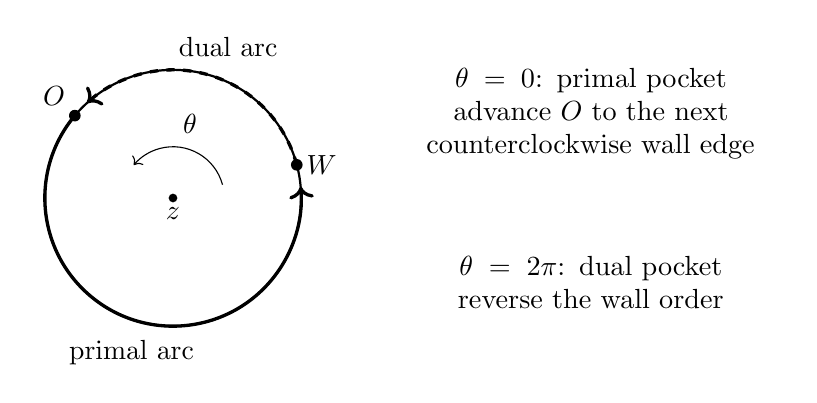
\begin{tikzpicture}[scale=1.05]
 \draw[thick] (0,0) circle (1.55);
 \draw[very thick,dashed,->] (15:1.55) arc (15:132:1.55);
 \draw[very thick,->] (140:1.55) arc (140:365:1.55);
 \fill (0,0) circle (1.5pt) node[below] {$z$};
 \fill (15:1.55) circle (2pt) node[right] {$W$};
 \fill (140:1.55) circle (2pt) node[above left] {$O$};
 \draw[->] (15:.62) arc (15:140:.62);
 \node at (77:.92) {$\theta$};
 \node at (70:1.95) {dual arc};
 \node at (255:1.94) {primal arc};
 \node[align=center,text width=4.8cm] at (5.05,1.02)
 {$\theta=0$: primal pocket\\
  advance $O$ to the next counterclockwise wall edge};
 \node[align=center,text width=4.8cm] at (5.05,-1.02)
 {$\theta=2\pi$: dual pocket\\
  reverse the wall order};
\end{tikzpicture}
\caption{Normalized chart of a two-change component.  The angle
$\theta=O-W$ is measured counterclockwise along the dual arc.
The arrows on the circle indicate boundary order, not strand
orientation.  The forcepoint reset uses the next old-wall edge on the
retained pocket.  A full turn changes the endpoint of the reflected
angular interval.  The drawing is schematic; microscopic tip and
force sides are suppressed.}
\label{tree:figure}
\end{figure}


Away from coincidences use Lemma~\ref{tree:interior}.  In an endpoint
zone, a fast exit toward the interior is controlled by the tightness
of $\theta$, and fast motion remaining in that zone is controlled by
Lemma~\ref{tree:bar} and the sign of $O$.  Thus $W$ and $O$ are
continuously tight, also at variable stops.  Moreover, on a sufficiently
small fixed endpoint zone, both the continuous part of $O$ and every
reset have the same sign.  Its variation on each visit is bounded by
its angular oscillation there.  Count visits by alternations between
nested endpoint zones, whose number is tight; outside these zones the
cotangent rate is bounded.  We obtain tightness of
\begin{equation}\label{tree:variation}
 \operatorname{Var}_{[0,T]}(O)
 \quad\hbox{and}\quad
 \int_0^T|\cot(\theta_t/2)|\,dt.
\end{equation}
In any limit the endpoint sets have zero radial Lebesgue measure,
$O$ has locally finite variation, and \eqref{peel:force-ode} holds off
those sets.  A remaining singular part could only be nonnegative at
$0$ and nonpositive at $2\pi$.  We next rule it out.

\subsection{Instantaneous reflection and removal of a singular push}
\label{tree:endpoints}

\begin{proposition}[The endpoint convention is determined]
\label{tree:reflection}
In its own radial clock, the limiting gap is the unique instantaneous
reflected diffusion on $[0,2\pi]$ with interior generator
\begin{equation}\label{tree:generator}
 \mathcal A f(\theta)=\frac\kappa2 f''(\theta)
       +\frac{\kappa-4}{2}\cot(\theta/2)f'(\theta).
\end{equation}
The forcepoint has no singular push:
\begin{equation}\label{tree:no-push}
 O_t=O_0+\int_0^t\cot(\theta_s/2)\,ds.
\end{equation}
Equation~\eqref{tree:sde} consequently holds globally, including
collisions, with locally integrable drift.
\end{proposition}

\begin{proof}
For a smooth function constant near both endpoints, the localized
interior identities glue to the martingale problem for
$\mathcal A$.  To admit a smooth function with
$f'(0)=f'(2\pi)=0$, approximate it by such cutoffs with uniformly
bounded second derivatives.  Its cotangent term is bounded near the
ends, since $|f'(\theta)|=O(\min(\theta,2\pi-\theta))$.
The endpoint time is zero, so dominated convergence gives the limiting
martingale identities and, by applying the same argument to $f^2$,
their brackets.

In particular $X=\cos(\theta/2)$ solves
\begin{equation}\label{tree:jacobi}
 dX_t=\frac{\sqrt\kappa}{2}\sqrt{1-X_t^2}\,dB_t
           -\frac{3\kappa-8}{8}X_t\,dt,
 \qquad -1\le X_t\le1.
\end{equation}
The diffusion coefficient is one-half H\"older and the drift is
Lipschitz; the one-dimensional square-root uniqueness criterion gives
pathwise uniqueness.  Hence this equation fixes the instantaneous
reflected law of $\theta$; a sticky alternative is also excluded by
zero endpoint time.

Near either endpoint the scaled distance $R$ has Bessel dimension
\begin{equation}\label{tree:bessel-dimension}
 \mathfrak d=3-\frac8\kappa\in(1,2).
\end{equation}
Its drift differs from $(\mathfrak d-1)/(2R)$ by a bounded smooth
term of order $R$.  Stopped Girsanov, equivalently in the squared
coordinate where the excess drift divided by the diffusion coefficient
extends boundedly, transfers the usual Bessel path properties.  Thus
$\theta$ is locally H\"older of every exponent below $1/2$, and each
endpoint set has Hausdorff dimension at most
\begin{equation}\label{tree:zero-dimension}
 d_0=1-\mathfrak d/2<1/2.
\end{equation}
The needed Bessel H\"older statement is, for example,
\citet[Theorem~1.2 and Corollary~2.14]{HutzenthalerJentzenNoll2014}.
The zero-set statement follows from the inverse-local-time description
in \citet[Section~2.2, p.~21]{Bertoin1999Subordinators} and the
stable-range dimension in \citet[Corollary~5.3, p.~42]{Bertoin1999Subordinators}.  Only a bounded stopped
perturbation at one endpoint is being used here.

Write the possible remaining term as the signed measure
\[
 d\nu=dO-\cot(\theta/2)\,dt.
\]
It is supported on the two endpoint sets and has the sign specified
after \eqref{tree:variation}.  We give the time-block argument
explicitly, so that a Hausdorff-dimension bound, rather than an unstated
Minkowski bound, suffices.  Choose $\eta>0$ so small that
\[
 p=\tfrac12-\eta>d_0,
 \qquad u_m=2^{-m},\qquad r_m=u_m^p.
\]
By the H\"older property, every sufficiently fine dyadic block of
length $u_m$ meeting an endpoint set has its end-gap at most $r_m/32$
throughout.  Indeed choose a H\"older exponent strictly between $p$
and $1/2$.  Apply Lemma~\ref{tree:bar} with harmless fixed buffer
changes to the finitely many blocks at level $m$, taking the mesh
limit first.  The probability that some level-$m$ block stays in the
stated endpoint zone and has one-signed $O$-variation exceeding $Cr_m$
is at most
\begin{equation}\label{tree:block-sum}
 C(1+T/u_m)\exp(-c u_m^{-\eta}).
\end{equation}
This is summable in $m$.  The estimate for $O$ follows from that for
$W$ because their difference is the end-gap, of size at most $r_m/32$
on such a block.  Borel--Cantelli gives, almost surely, the variation
bound $Cu_m^p$ on every sufficiently fine endpoint-meeting block,
separately for the two endpoints and on each fixed horizon.

On an endpoint neighborhood, $dO$ is one-signed, and so is the
cotangent time measure.  Its restriction to the endpoint set is zero,
whereas the restriction of $dO$ there is precisely $d\nu$.
Consequently $|\nu|(I)\le\operatorname{Var}_I(O)$ for every small
interval in that neighborhood.  Cover the endpoint set by intervals
of variable lengths whose sum of $p$th powers is arbitrarily small,
using \eqref{tree:zero-dimension}.  Replace each by a bounded number
of comparable dyadic intervals that meet the set.  The preceding
variation bound yields arbitrarily small $|\nu|$-mass.  Thus
$\nu=0$, proving \eqref{tree:no-push}.

Finally, a Bessel process of dimension greater than one is a
semimartingale with integrable inverse-distance drift and no local-time
term in its ordinary coordinate
\citep[Lemma~3.2]{HutzenthalerJentzenNoll2014}.  Undoing \eqref{tree:jacobi} in the
endpoint neighborhoods, and using the interior identities elsewhere,
gives
$d\theta=-\sqrt\kappa\,dB+((\kappa-4)/2)\cot(\theta/2)dt$.
Together with \eqref{tree:no-push} this is \eqref{tree:sde} globally.
There is therefore no unspecified boundary pushing rate.
\end{proof}

\subsection{Common clocks and independence after separation}
\label{tree:joint}

The single-branch conclusion does not by itself identify the joint
tree.  In particular a narrow discrete corridor may survive after its
two limiting target kernels have separated.  We address this before
using any continuum tree theorem.

\begin{proposition}[Joint target tree]\label{tree:joint-law}
For every finite family of deterministic interior targets, the peeling
converges in its joint radial driving data to the target-invariant
branching radial $\mathrm{SLE}_\kappa(\kappa-6)$ tree.  Branches agree
until their target kernels separate and then have independent
continuation noises.  At successive full turns the force side is
reversed, equivalently the angular gap remains instantaneously
reflected on $[0,2\pi]$.
\end{proposition}

\begin{proof}
Use the sum of currently accrued target clocks as a common parameter
$v$, freezing each target at its prescribed horizon.  Every clock
$t_i(v)$ is nondecreasing and $1$-Lipschitz.  Several run together while
their targets share an active component; separate components are
processed in serial priority order.  A flat clock has a constant state.
All tightness bounds and the interior identities hold between adapted
common-clock stops, including tests of the whole past.  Work in other
components during an interrupted segment is conditionally independent
of its unqueried switches by Lemma~\ref{peel:factorization}; neither
the schedule nor the stop gives advance information.

Extract limits jointly with the clocks.  The preceding endpoint
arguments can be applied in each marginal's own radial clock, using
tightness and inverse-clock extraction across flat stretches.  Thus
the martingale part $M_i$ of $W_i$ is a continuous local martingale
relative to the common past, with
\begin{equation}\label{tree:brackets}
 d\langle M_i\rangle=\kappa\,dt_i.
\end{equation}
The Loewner equations determine its target kernels and normalized
maps.

While targets $z_i,z_j$ remain in one component, put
$\xi=\Phi_i(z_j)$.  Radial Loewner evolution and the conformal-radius
change give
\begin{equation}\label{tree:clock-change}
 dt_j=P^2\,dt_i,\qquad
 d\log|\xi|=P\,dt_i,\qquad
 P=\frac{1-|\xi|^2}{|e^{iW_i}-\xi|^2}.
\end{equation}
Their marked boundary angles correspond by the normalized disk
M\"obius map.  On a compact interval with $|\xi|<1$ these formulas
are regular and pass to the limit.  The targets are still in the same
kernel exactly while they retain an interior connecting path: kernel
convergence preserves paths with positive clearance.  Thus they have
the same growth up to kernel separation.

Suppose now their limiting kernels have separated but their discrete
components have not yet split.  Along such a portion $|\xi|\to1$ by
monotonicity.  On a subinterval where both limiting angle gaps stay in
the interior, the two marked prepoints remain separated in both
charts.  To see the resulting clock separation explicitly, set
$w=e^{iW_i}$, $o=e^{iO_i}$ and $F_\xi(u)=(u-\xi)/(1-\overline\xi u)$.
The disk M\"obius identity is
\[
 |F_\xi(w)-F_\xi(o)|
 =\frac{(1-|\xi|^2)|w-o|}{|w-\xi|\,|o-\xi|}.
\]
If both chord gaps are bounded below, the product in the denominator
is at most $C(1-|\xi|)$, while $|w-o|$ bounds the larger factor below.
Thus one of $w,o$ is within $C(1-|\xi|)$ of $\xi$.  The choice cannot
change on a connected interior-angle subinterval when $|\xi|$ is
sufficiently close to one.  If it is the tip, $P$ is of order
$(1-|\xi|)^{-1}$; if it is the forcepoint, $P$ is of order $1-|\xi|$.  Equation~\eqref{tree:clock-change}
then forces one limiting clock to be flat.  This remains true along
subsequences of exact discrete split times.  After an exact split,
serial growth gives disjoint time interiors for the two clocks.
The fixed-priority schedule has only finitely many target-group split
and freeze stages.  On each stage, exhaust the open set where both
angle gaps are interior by countably many compact subintervals; the
preceding clock-separation argument applies on each of them.
Endpoint angle sets have zero mass
for the corresponding own clock by Proposition~\ref{tree:reflection}.
The covariance inequality for continuous local martingales and
\eqref{tree:brackets} therefore show that
\begin{equation}\label{tree:orthogonal}
 d\langle M_i,M_j\rangle=0
 \quad\hbox{after their kernel separation}.
\end{equation}
Frozen targets are omitted from this comparison.

We spell out why these characteristics determine independent
continuations, without asserting that the clocks are independent.
In each still-accessible active group choose its first indexed target
as representative.  Until a separation or freeze, the representative's
motion determines all other states and clocks by
\eqref{tree:clock-change}.  Separation and freeze times are intrinsic
stopping stages: mutual accessibility is read from the radial ODE up
to first approach to unit modulus.  While two other members remain
regular with the representative, they cannot lose their shared access
before either is lost from that representative.  A nonrepresentative's
horizon is likewise read by its clock correspondence.  At a multiple
separation, take the continuous state limits in all own clocks; the
subgroups are exactly those retaining internal mutual paths in their
kernels.  Serial speeds of unrelated groups have no effect on these
stages.

For each target accumulate its martingale coordinate only over the
suffix during which it is an active representative, keeping it flat
otherwise.  More precisely, with the predictable choice at the stage
endpoints, set
\[
 N_i(v)=\int_0^v
 \mathbf 1_{\{i\text{ is an active representative at }s\}}\,dM_i(s).
\]
Once it becomes representative it remains representative of its
descendant group until it freezes.  These representative martingales
$N_i$ are pairwise orthogonal by \eqref{tree:orthogonal}.
Their terminal brackets can be finite, so make the completion explicit.
Let $T_i$ be the prescribed horizons and take the deterministic common
terminal parameter $V=\sum_iT_i$, extending all stopped states constantly
if necessary.  Divide each $N_i$ by $\sqrt\kappa$, and enlarge the
common filtration after $V$ with
independent Brownian motions $\widehat B_i$, independent also of the
entire original terminal sigma-field.  Set
\[
 \widehat N_i(V+s)=N_i(V)/\sqrt\kappa+\widehat B_i(s),\qquad s\ge0,
\]
and use $\widehat N_i(v)=N_i(v)/\sqrt\kappa$ for $v\le V$.
The extended processes are continuous local martingales in this
enlarged common filtration, remain pairwise orthogonal, and have
infinite terminal brackets.  Knight's orthogonal-martingale time-change
theorem now gives independent standard Brownian motions in their
respective bracket clocks
\citep[Theorem~2, p.~191]{Meyer1971Knight}.
Restricting to each original terminal bracket supplies precisely its
original representative martingale.  The auxiliary continuation changes
neither the past filtration nor any stage of the exploration.

For the conditional assertion, let $\mathcal G_v$ be the common causal
filtration and let $S$ be a separation or freeze stage.  Restart the
active representative martingales at $S$, stop at the next common stage,
and pad constantly to a deterministic horizon.  After localizing to
bounded brackets, these restarted processes remain orthogonal
martingales under $\mathbb P(\,\cdot\mid E)$ for every $E\in\mathcal G_S$ of
positive probability, with the same bracket identities.  Completing
them as above and applying Knight's theorem under this measure gives
the same product Wiener law for every $E$.  Thus the continuation
noises are independent of $\mathcal G_S$.  A continuing representative
uses its original martingale increments, and a newly selected one
starts its representative suffix.  No conditioning on terminal
bracket values or future separation data is involved.

The pathwise uniqueness of \eqref{tree:jacobi}, followed by
\eqref{tree:no-push}, determines the angles and maps through the next
intrinsic stage.  A newly assigned representative uses its assigned
independent noise; a continuing one uses the continuation of the same
Brownian solution.  A change caused solely by a representative's
horizon gives a fresh continuation at that stopping stage.  Induction
over the finite target groups identifies the usual common-branch,
independent-after-separation construction.

The resulting equations and angular convention are the target-invariant
radial tree of
\citet[Propositions~3.13--3.14 and Section~4.2]{Sheffield2009Exploration}:
a one-sided force weight $\kappa-6$, with the side reversed in an
enclosed component after a full turn.  Our sign convention is
$\theta=O-W$; exchanging the sign of its Brownian motion translates
to the opposite angular convention.  Increasing the finite horizons
proves the assertion at all finite clocks.
\end{proof}

\section{Recovery of the nested loop collection}
\label{sec:loops}

We now identify the full loop curves encoded by the limiting
exploration tree, including their traversal order and multiplicity as
collection elements.  The argument first compares loops in a fixed
wired square and then transfers this identification to the free plane law.
Within the square, we first match loops by the dense-set targets they
surround.  Winding information then identifies their traces, and a
separate argument rules out additional traversal portions.  These are
distinct steps: agreement of surrounding-loop labels alone does not
identify either the complete trace or its order of traversal.

Continue first in a fixed axis-parallel square with the primal-open
wall and wired law of Subsection~\ref{peel:construction}.  Draw the two
pairs at each tile contact disjointly in a midpoint disk of radius
less than $\delta/100$, taking each turn on its prescribed side.
The resulting actual loops are simple, pairwise disjoint, and avoid
actual open diagonals of both colors.  Use the analogous drawing for
wall triangles and orient every loop primal-left.  Matching successive
traversal pieces inside those disks changes each loop by at most
$2\delta/100$ in Euclidean uniform curve distance, and by a constant
multiple of this in spherical distance, simultaneously for all loops.
Thus the drawing convention has no effect on the desired topology.

\subsection{Compactness and two sides of every limiting loop}
\label{loop:compactness}

\begin{lemma}[Positive-law loop geometry]\label{loop:geometry}
The closed loop collections in the fixed square are tight for matching
uniform curves modulo reparametrization and orientation.  Constant
limit curves may be removed.  Their positive-diameter subsequential
limits have the following properties almost surely.
\begin{enumerate}[label=\textup{(\roman*)}]
\item Each deterministic interior point lies on no loop.  Its absolute
winding number about any loop is $0$ or $1$, and is stable along a
converging loop sequence.
\item No interior point has three distinct visits in total among the
loop elements.  Visits include multiple traversals after constant
pauses are removed and also multiplicity of different elements.
\item At every interior point of a positive loop, every neighborhood
contains open disks of both absolute winding statuses for that loop.
\end{enumerate}
\end{lemma}

\begin{proof}
\textit{Passage counts and compactness.}
Consider a vertical band of fixed positive width, with its vertical
sides interior to the square and its height equal to that of the
square.  Each disjoint medial passage between its sides has an actual
dual path beside it: consecutive adjacent dual vertices are identical
or joined by an open dual diagonal, including at wall caps.  Crop to
a slightly narrower band.  The medial separators continue beyond both
cropped sides and are disjoint from dual-open edges, so they divide
the band into strips.  Each accompanying dual path lies in the strip
on its separator's dual side, with at most two assignments to a strip.
Paths in different such strips cannot communicate in the actual dual
graph there.  Hence many passages force many distinct actual dual
components crossing the cropped band.

The graph of internal dual faces is a full lattice rectangle with
arbitrary induced boundary data; it has no dual crossing of the
initial deterministic primal wall.  The disjoint-passage proof of
Lemma~\ref{peel:passages} bounds its crossing-component count.
Even with all boundary vertices wired, an \emph{actual} left-right
crossing is bounded away from probability one by an up-to-boundary
primal blocker.  End that blocker just beyond the extreme dual rows
by bounded finite-energy extensions to neighboring internal primal
vertices.  The rectangle's dual boundary edges themselves are random,
so the crossing theorem applies.  The same argument holds for
horizontal bands.

A finite family of trimmed bands at each fixed scale bounds both the
number of loops with diameter above that scale and the number of their
disjoint subarcs with a given positive displacement.  These bounds
yield compactness modulo reparametrization.  To make the extraction
explicit, subdivide each positive loop by successive first-displacement
times into arcs of diameter at most $2^{-j+O(1)}$, retaining marks from
previous subdivisions.  The number of marks at each fixed $j$ is
tight.  Pass to subsequences on which their positions and cyclic orders
converge.  Assign nested parameter intervals with maximal length
tending to zero and positive lengths at every fixed subdivision,
splitting an interval further in two when necessary.  The corresponding
polygonal curves approximate uniformly.  Diagonalize over diameter
cutoffs tending to zero, retaining multiplicities of matched elements.
This proves collection tightness.

\paragraph{Avoidance and the visit bound.}
For a deterministic interior point, RSW circuits in successive
concentric annuli obstruct an actual arm to a fixed positive distance.
The probability that a macroscopic loop approaches that point tends
to zero with the inner radius.  A countable union over diameter
cutoffs gives (i).  Winding is stable under uniform convergence away
from the point, and each simple discrete loop has absolute winding
$0$ or $1$.

Three distinct positive visits near an interior point would yield six
medial passages through arbitrarily small annuli out to a fixed
positive scale.  This includes visits belonging to different collection
elements.  In a trimmed intermediate annulus, order those radial
separators and assign their actual color arms to the intervening
strips.  Arms in distinct strips stay separated.  Where a strip
receives two assignments retain both if their colors differ, and one
if their colors agree.  Each separator marks a color transition, so
the resulting cyclic sequence has an alternating subfamily of at
least six arms.  Radial buffers justify all croppings.  The six-arm
bound of \citet[Corollary~6.7]{DMT2021Fractal}, transferred to this
positive square law through a bulk collar, has exponent $2+c$ for
some $c>0$.  A grid union over possible centers therefore vanishes
like a positive power of the inner scale.  Taking mesh limits first
proves (ii).

\paragraph{A circuit attached to each macroscopic bank.}
Fix a bulk core rectangle, with buffer space around it, and a color
$X$.  We claim that, with probability tending to one as $m\to\infty$
after the mesh limit, the actual cluster of every bottom-to-top core
crossing contains an $X$-open circuit in the buffered patch enclosing
a disk of radius $c/m$.

In a first subrectangle ending at a middle row, label the actual
connected components joining its two terminal rows.  Their number is
tight by the passage bound.  Reveal the past up to that middle row.
Above it use $m$ fresh transverse slabs of height $h\asymp1/m$,
with all levels rounded on the $X$-grid.  For a given label, its
sources are its actually connected bottom vertices.  At each new row
ask whether these sources connect to that row in the cumulative core
rectangle.  A full crossing survives all these tests under one of
the initial labels.

When a label survives to a row, choose the leftmost simple open path
from its sources to that row.  The edges strictly to its right are
fresh with domain Markov data.  Indeed attach auxiliary spokes from
one point below to the sources and from the new top row to a point
above, in a disk with these auxiliary endpoints on its boundary.
Simple paths use spokes only at their ends.  Minimizing left area
selects a path determined by its own edges and those on its left:
any path entering strictly left supplies an open excursion between
two distinct selected-path vertices that decreases the left region.
The ordinary lattice part $p$ is actually connected to the label.

At the slab's middle height, approach horizontally from the right
exterior of the core and choose $x$ on the right at distance $h/16$
from $p$.  The ball $B(x,h/3)$ lies in the wider fresh patch, far
from the past, spokes, and slab ends.  The fresh graph on the right
of $p$ inside a slightly buffered ball dominates the restriction of a
free comparison on the full ball graph.  All attachments from omitted
left-side or path edges go through vertices of $p$, which are wired
by actual connectivity in the conditioned law.  This argument applies
to either color, using the dual FK law for dual $X$.

By interior RSW and FKG in the free ball comparison, with probability
at least a fixed $c'>0$ there is an open circuit between radii
$h/64,h/24$, connected there to one between radii $h/8,h/4$.
The outer circuit meets the deterministic geometric path $p$, since
$p$ comes within $h/16$ of $x$ and exits the ball.  Both use the same
color graph.  The inner circuit is wholly on the right of $p$, as is
its connection up to first contact with $p$.  Therefore this event
supplies an actual attached disk-circuit using only fresh right-side
edges in the slab.  Conditionally on survival, failure to acquire such
an attachment costs a factor at most $1-c'$ at each stage.  Truncate
the initial number of labels and iterate.  This proves the claim.

\paragraph{Visibility of both winding statuses.}
Use countably many core tests with rational positions and buffered
sizes.  A varying portion of a limiting loop in an interior ball
crosses two horizontal or vertical levels of one such test with
clearance.  In its discrete approximants the two actual color banks
supply crossings.  Their clusters lie on opposite sides of the simple
loop and do not cross it.  Choose the buffered test much smaller than
the loop's diameter, so neither of the attached disk-circuits can
contain the entire loop.  The disks strictly inside the two circuits
then have the two corresponding winding statuses.  Shrink them to
retain positive clearance; subsequential limits preserve disks of
positive radius in the prescribed ball.  The preceding estimate makes
failure arbitrarily unlikely.  Every neighborhood of a point on a
nonconstant loop contains a varying portion, so the countable tests
prove (iii) simultaneously.
\end{proof}

\subsection{Canonical loops and their continuation in the tree}
\label{loop:canonical}

Take joint subsequential couplings of the loop collections and of the
angular trees for a countable dense set $\mathcal Z$ of deterministic
interior targets, with arbitrarily large finite clock horizons.
Lemma~\ref{loop:geometry}(i) ensures that all these targets avoid all
positive limiting loops almost surely.  Incidental lattice-edge
positions do not require an extra convention: each active finite
horizon retains a ball around its target.

We specify the established continuum input before making the lattice
identification.  For $4<\kappa<8$, the target-invariant tree of
\citet[Sections~4.2--4.3]{Sheffield2009Exploration} constructs the
surrounding loops by full-turn angular excursions and completes each
partially traced loop through the other branches.  At the time of
that paper, its stated continuity and invariance conclusion in
Proposition~5.1 was conditional.  Here the needed hypotheses follow
from \citet[Theorem~1.3]{MillerSheffield2016IG1} and
\citet[Theorem~1.2 and the ensuing CLE discussion]{MillerSheffield2016IG3}.
For our single one-sided force weight, $\kappa-6>-2$, so force
collisions do not reach the continuation threshold.  For reversal,
the two one-sided weights $\kappa-6$ and $0$ are both at least
$\kappa/2-4$.  The starting square is a Jordan domain, and all
specified targets are distinct interior points off the loops.  These
results supply continuous non-simple CLE loops and their conformal
and anticonformal invariance under exactly the parameters used here.
They assert no lattice convergence or traversal identification.

The tree in Proposition~\ref{tree:joint-law} therefore has a coupled
canonical nested $\mathrm{CLE}_\kappa$ collection in the square.
Starting from a primal wall, let $b_0=0$, and let $b_1,b_2,\ldots$
be the successive hits of the alternating opposite endpoints:
first $2\pi$, then $0$, and so on.  Let $a_k$ be the last visit to
the starting endpoint before $b_k$.  The canonical surrounding loop
is denoted $\widetilde L_z^k$.  It follows the branch toward $z$ on
$(a_k,b_k)$ and is then completed to its starting point by the tree's
continuation of the current strand.  These are the successive loops
with nonzero winding about $z$, and every canonical loop is obtained
from a target in $\mathcal Z$.

The endpoint reversal amounts to using reflected exploration chirality
in the new enclosed component.  Nesting supplies independent CLEs in
those components, and anticonformal invariance preserves their
unoriented laws.  Thus the alternating endpoint convention gives the
same nested ensemble.  The scalar full-turn description is also the
one in \citet[Proposition~2]{SchrammSheffieldWilson2009}; that result
identifies the conformal-radius decrement, while the joint branch
coupling and loop completion used here come from the exploration-tree
construction.  Endpoint accessibility of the diffusion with
$1<\mathfrak d<2$ makes every $b_k$ finite, and $b_k\to\infty$:
otherwise its continuous angle would make infinitely many full
$2\pi$ swings on a compact clock interval.

We will need the following concrete interpretation of the completion.

\begin{lemma}[Default continuation and local double visits]
\label{loop:continuation}
At an interior-angle time $s\in(a_k,b_k)$, the remaining traversal
of $\widetilde L_z^k$ is the default strand from $W_s$ to $O_s$ in
the current domain.  In a chart sending those accesses to $0,\infty$,
every finite portion of this continuation is ordinary chordal
$\mathrm{SLE}_\kappa$ and is recorded by branches to targets from
$\mathcal Z$ that remain accessible high above that portion.
Every open nonconstant traversal interval of $\widetilde L_z^k$
contains two visits to one square-interior point.
\end{lemma}

\begin{proof}
The stopped chordal equivalence is only valid while its force access
is available.  To continue after the original target is cut off, use
the branch that retains this access, as prescribed by the tree
construction.  A bounded finite chordal-capacity portion has bounded
hull and driver.  An open set of targets mapped to sufficiently large
heights remains accessible above it, with tip and force angles strictly
separated on that portion.  The countable dense set supplies such a
target.  Its branch records the default continuation even if it has
already separated from $z$.  Target invariance gives consistency when
the target or the finite portion is enlarged.  This realizes all
finite portions and hence the complete strand; it does not extend
Proposition~3.12 of \citet{Sheffield2009Exploration} beyond its stopping
condition.

For a single branch stopped at a finite radial time, its continuous
trace together with the starting square boundary is a locally connected
planar continuum.  The current target domain is a complementary
component of this continuum.  Torhorst's theorem says that every
complementary domain of such a continuum has locally connected boundary.
The Riemann map from the disk onto that domain therefore extends
continuously to the closed disk
\citep[historical comments and Corollary~3.2]{RempeGillen2008PrimeEnds}.
Thus the prime-access conformal images used here are continuous
physical curves.

For ordinary chordal SLE, \citet[Theorem~1.1 and Corollary~1.7]{MillerWu2017}
give double points in the interior when $4<\kappa<8$.  Indeed their
double-point dimension exceeds the boundary-hit dimension by
$(\kappa-4)^2/(8\kappa)>0$.  Both visits occur at finite times.
Scaling makes the probability of such a double visit before time $t$
independent of $t>0$; since its union over finite times has probability
one, this probability is one for every $t>0$.  The domain Markov
property then gives an interior double visit in every rational open
capacity interval.  Conformal maps preserve an interior double visit.
Arrange a single probability-one event over all targets $w$ in the
fixed countable dense set, all rational $w$-clock times $r$, and a
countable exhaustion of strict angle and chart localizations.  The
first time that the $w$-clock reaches $r$ is causal.  Conditional
stopped chordal equivalence and the simultaneous rational-interval
double-visit property therefore apply until its positive localization
exit.  Every open interval of a full-turn piece contains such a
rational start.

For an interval in the default completion, choose a rational time $s$
in the original successful excursion and a finite chordal portion
containing a compact subinterval of the desired interval.  As above,
a target $w$ from the same countable set at sufficiently large chart
height records that portion with interior angle, even after the
original target is cut off.  Its radial and chordal clocks are strictly
increasing there, so the subinterval contains a rational $w$-clock
start.  The universal probability-one event permits this
realization-dependent choice of $w$ and $r$.  Applying the local
double-visit property before its positive exit time proves the
assertion.  No Markov property is applied at a non-stopping excursion
start or at an arbitrary postselected time.
\end{proof}

\subsection{Episodes and full-turn labels}
\label{loop:episodes}

A discrete \emph{episode} starts when a cap is opened and ends at the
next switch retaining a homogeneous pocket.  Its color is the
homogeneous wall color just before the opening.  Call it successful
when its loop winds around the target.

\begin{lemma}[Discrete winding order]\label{loop:episode-order}
As long as the target is macroscopically separated from a consumed
tile or star, an episode is successful exactly when its terminal
switch changes wall polarity.  These polarity changes enumerate all
loops surrounding the target, in their order from outside inward.
A positive loop with positive clearance from the target is reached
before a finite radial horizon depending on that clearance.
Conversely a successful switch by a bounded horizon has macroscopic
clearance from the target.
\end{lemma}

\begin{proof}
The loop through the newly opened cap lies inside its homogeneous
starting pocket.  At the cap, the side toward the base, of the
starting color, is exterior to this loop; the other side is interior.
During the episode the actual color banks preserve connections to
these sides.  If a bank hits its same-color wall, the retained
homogeneous target pocket is connected to the cap along that bank.
The traversed loop is outside the pocket: its past pairs have been
removed, the new open diagonal is a barrier, and the continuation to
the old force side stays in the main component.  The target can reach
that pocket's wall color without crossing the loop.  Comparing this
color with the starting color proves that the target is inside the
loop precisely at a polarity change.  The same argument works with
separate boundary occurrences.

Every other unstarted candidate surrounding the target stays intact
in the retained component.  Actual diagonals and walls cannot cross
it, and a loop wholly inside a simply connected pocket has its
interior there too.  Its deterministic pairs in any wall triangles
are also intact, because cuts by other loops never traverse them.
If the loop entered at a new cap surrounds the target, it is outermost
among the remaining candidates: its access to the homogeneous wall
at that cap crosses none of them.  Thus successful episodes enumerate
the surrounding loops, with possible unsuccessful same-color episodes
between them.

Before such a loop's episode, growth remains outside its enclosed
region; during the episode it follows that loop up to step-sized
errors.  A ball centered at the target inside its region therefore
survives until the switch.  If its radius is $r>0$, then
$\operatorname{crad}(U_t,z)\ge r$ up to that time, bounding the
radial clock by $\log(\operatorname{crad}(U_0,z)/r)$.
Conversely, Koebe's bound on a fixed horizon gives a positive-radius
ball in the newly retained pocket, and its surrounding successful
loop lies outside that ball, up to vanishing step errors.
\end{proof}

An endpoint approach could otherwise be mistaken for a reset in the
limit.  The next estimate excludes this possibility.

\begin{lemma}[Endpoint resets cannot be skipped]
\label{loop:no-skip}
At a bounded-clock completed state with $\theta$ approaching $0$,
the probability of returning to a fixed positive angle before a
primal-pocket reset tends to zero, with the mesh limit first and the
endpoint tolerance second.  The analogous assertion near $2\pi$
uses a dual-pocket reset.  Consequently the true successive discrete
polarity-change times $b_k^n$ converge in probability to $b_k$ on
sufficiently large finite horizons.

Moreover, in an episode that succeeds by a bounded horizon, after a
fixed interior-angle advance the probability of retreating arbitrarily
near its starting endpoint before its successful switch tends to zero
in the same order of limits.
\end{lemma}

\begin{proof}
Near $0$ the entire dual wall arc and both end sides are in a tiny
boundary neighborhood of the stopping chart.  Until a primal reset,
the growing dual bank remains actually connected to that arc; stop
also before a fixed interior-angle threshold, so no opposite-end
switch has yet occurred.  In successive buffered dyadic chart
half-annuli around this neighborhood, place actual primal transversal
paths from primal wall to primal wall.  Lemma~\ref{peel:wall-rsw}
gives a uniformly positive conditional success chance at each
separated scale, after the mesh limit at the chosen cutoffs.  A
successful path confines the connected dual bank, and hence the slit
pieces, inside its small wall sector.

A hull confined to such a sector has a small new angular footprint:
its basepoint-side maps converge to the identity at the origin and,
by reflection, on each closed boundary arc away from that sector.
The trapped dual arc remains in its short footprint.  Therefore it
cannot produce a fixed positive angular advance.  Letting the number
of half-annuli grow proves the first assertion.  Exchange colors and
reverse directions at $2\pi$.

A true polarity change approaches the specified opposite endpoint,
up to vanishing update errors.  Uniform angle convergence and induction
therefore preclude a premature macroscopic limit for $b_k^n$.
Conversely, after the limiting first endpoint hit, instantaneous
reflection produces a positive excursion within any prescribed
additional time almost surely.  Truncate the clocks and choose an
exit size so that failure has arbitrarily small probability.  Start
at the first completed-state approach within a small tolerance after
the previous true polarity change.  The just-proved estimate excludes
an excursion of this size before the corresponding reset.  Let the
tolerance tend to zero.  An earlier matching reset already suffices.
Thus no endpoint hit is skipped, and $b_k^n\to b_k$.

For the final assertion, stop at successive approaches to the starting
endpoint after a fixed-size advance.  A successful episode that makes
such an approach must then advance macroscopically without the
corresponding same-color reset, since that reset would end the episode.
The first assertion bounds each such event.  The number of fixed-size
swing tests is tight by angular tightness, so truncation and iteration
give the stated retreat estimate.
\end{proof}

It follows in particular that on every compact subinterval of
$(a_k,b_k)$, the prelimit target branch is, with probability tending
to one, in the same episode as at its $k$th successful switch.  The
angle stays away from the starting endpoint on that compact interval,
and the preceding polarity change occurs before it.

Include the true winding-loop labels $L_z^{n,k}$ in the coupling and
extract their limits $L_z^k$, increasing clock and diameter cutoffs
as needed.  They have positive size at bounded $b_k^n$ by
Lemma~\ref{loop:episode-order}.  They exhaust the positive limiting
loops winding about $z$: any such loop has positive clearance from
$z$ and is reached before a bounded horizon, while the number of full
swings there is tight.  Winding tests are stable.  For finite lists of
labels stabilize also the indicators of equality as collection
elements and then diagonalize.  Distinct elements in this bookkeeping
have distinct discrete representatives, even if their geometric limits
might initially appear identical.

\subsection{Ordered containment and equality of the labels}
\label{loop:matching}

\begin{lemma}[The canonical traversal is contained in order]
\label{loop:ordered}
For each $z\in\mathcal Z$ and $k\ge1$, the entire traversal of
$\widetilde L_z^k$ occurs in cyclic order in $L_z^k$, possibly with
extra traversal portions inserted.  Its order occupies at most one
turn of $L_z^k$.  If two canonical labels give the same element, their
lattice-limit labels give the same collection element.
\end{lemma}

\begin{proof}
Fix a rational $s\in(a_k,b_k)$.  In any open subinterval of
$(a_k,s)$ choose $t<t'$ strictly inside it.  The target kernel strictly
shrinks between these times.  There is a new boundary point inside
the earlier open kernel; it belongs to the continuous canonical trace
over $[t,t']$.  Every small ball about this point with closure in the
earlier kernel must encounter new prelimit growth between the
corresponding times.  Otherwise the ball stays clear of new boundary.
It also meets a compact internal patch of the later kernel.  Connectedness
then puts that whole ball in the retained prelimit component, extending
the limiting kernel through its alleged boundary point, a contradiction.
These prelimit boundary pieces are slit updates tracing the successful
episode, up to vanishing physical step errors.

Apply this test simultaneously to any finite ordered list of such
intervals.  Completed-update stops can be moved slightly inside them
because capacities and angular within-step errors vanish.  We obtain
points of the discrete winding-loop traversal, in chronological order,
converging to canonical trace points in those intervals.

Now take any finite list of finite chordal intervals on the default
continuation after $s$.  Choose, realization by realization, a target
$w\in\mathcal Z$ in the current kernel whose chart image is safely
above the entire bounded portion in question.  It was still accessible
with $z$ up to $s$.  Their time correspondence there is regular and
passes to the mesh; they cannot have split earlier because the limiting
kernel contains internal connecting paths with clearance.  The branch
toward $w$ follows the default continuation with tip and force angles
separated by a positive margin on the selected portion, by
Lemma~\ref{loop:continuation}.  Therefore its discrete branch has no
reset there and continues the same original winding loop, in order,
after the common prefix.  The new-boundary test applies to these
intervals in the $w$-clock.  The target $w$ need not have a successful
episode for this loop.  Its post hoc choice costs no uniformity
assumption: all targets, clocks, and regular sharing correspondences
from the countable set have already been included in the coupling.

By continuity, shrinking the testing intervals and increasing the
finite continuation range shows that every finite increasing list of
canonical traversal points has representatives in order on $L_z^k$.
On a countable dense set of canonical parameter values, take a
single nondecreasing cyclic choice of representative parameters by
compactness and a diagonal subsequence.  Omitted endpoint values are
included by continuity.  The order uses at most one turn: the discrete
episode and its no-reset continuation traverse a simple closed loop
from its released cap without passing that cap a second time.
Two separated canonical visits cannot collapse to one representative
parameter, because every intervening open traversal interval has
actual variation.

If $\widetilde L_z^k=\widetilde L_w^j$ but the two lattice-limit
elements were distinct, each would contain the same canonical
interior double visit from Lemma~\ref{loop:continuation}.  This would
give more than two total limiting visits at that point, contrary to
Lemma~\ref{loop:geometry}(ii).  Thus equal canonical labels have equal
lattice-limit labels, with multiplicity understood as stipulated above.
\end{proof}

The converse is essential: ordered containment alone would permit
several canonical labels inside one discrete limiting element.

\begin{lemma}[The converse label identification]
\label{loop:label-equivalence}
With equality understood as equality of collection elements, almost surely
and simultaneously for all $z,w\in\mathcal Z$ and
$k,j\ge1$,
\begin{equation}\label{loop:label-iff}
 L_z^k=L_w^j
 \quad\Longleftrightarrow\quad
 \widetilde L_z^k=\widetilde L_w^j.
\end{equation}
\end{lemma}

\begin{proof}
Only the forward implication remains.  On the event that the discrete
labels are shared, the two branches cannot split before entering this
common loop: before its episode the loop and its interior remain
intact across every cut by other loops.  Choose clock horizons large
enough to include both successful switches except on an arbitrarily
small event.

While they share a domain, write $\xi=\Phi_z(w)$.  For a fixed small
$e>0$, stop at first approach to $|\xi|\ge1-e$, if it occurs before
the relevant winding switches.  For fine mesh this can be a completed
state also satisfying $|\xi|\le1-e/2$.  An exact split cannot precede
this threshold inside the comparison range: the ODE and clock change
are regular for $|\xi|\le1-e/2$, and elementary capacities vanish
there.

We first show that an \emph{unstarted} loop surrounding both targets
at this stop has probability tending to zero as $e\downarrow0$.
Place separated dyadic chart half-annuli around the boundary direction
of $\xi$, between radius a multiple of $e$ and a fixed small radius.
Choose their buffered wall intervals to avoid the two marked accesses
and sides; deleting the bounded number of affected scales leaves a
number tending to infinity.  Each bar separates a sector containing
the radial access from $w$ to the wall from the sector containing $z$
and a remote wall portion.

Use an actual-color transversal path in each bar, choosing the color
to match one wall end.  At that end it reaches an actual wall vertex.
At the other it does so as well if the wall has the same color.  If
that wall has the other color, complete the path from its specified-color
triangle corner to the base by the segment of
Lemma~\ref{peel:wall-rsw}.  After trimming at first wall contacts this
is a simple crosscut in the prime closure.  Its added segment meets
only the one local cap pair, once.

An unstarted simple loop inside the domain surrounding both targets
must cross this screen at least twice: it must meet both of the
separated sectors, and its interior contains both targets.  It cannot
cross the actual open path, and cannot traverse that one cap pair
twice.  Thus one successful screen precludes the event, even with
mixed wall colors.  The conditional success probability of each
fixed-aspect buffered bar is bounded below by
Lemma~\ref{peel:wall-rsw}.  Iteration, with the mesh limit first,
proves the asserted small probability.

We next obtain a shared interior precursor for a shared successful
loop.  If the common loop is processed before the near-separation
threshold is needed, its episode visibly passes through interior
angles, comparable in the two charts while $|\xi|\le1-e/2$.
If the loop is still current at the threshold, its $z$-angle cannot
be arbitrarily close to that episode's starting endpoint and later
succeed without a same-color reset, by Lemma~\ref{loop:no-skip}.
Otherwise, its progression from the start to the current state has
already passed a fixed interior margin.  The $w$-angle at that shared
state has a comparable interior margin, with constants allowed to
depend on $e$.  The unstarted case has just been made unlikely.
Thus, except on an arbitrarily small event, the two successful
episodes have a common state before kernel separation, with both
angles interior by fixed positive margins.

From this precursor to the respective winding switches, neither angle
returns arbitrarily near its episode's starting endpoint, by the
successful-episode retreat estimate in Lemma~\ref{loop:no-skip}.
Choose in order the clock cutoff, the near-separation threshold, the
interior margins, and the retreat tolerance, making their error
probabilities successively small.  With strict buffers a subsequential
precursor remains in a common kernel with $|\xi|\le1-e/2$, lies after
both previous polarity changes, and lies in the interiors of both
limiting successful excursions.  Their endpoint histories and starting
excursion time agree along the common branch by the regular chart
correspondence.  They share the successful front to this interior
state and use the same default continuation to the same force access
for its rest.  Therefore their canonical loop elements coincide.
Let all the preceding errors tend to zero.  Countability of the
labels proves the simultaneous assertion.
\end{proof}

\subsection{Trace and traversal identification}
\label{loop:traversals}

We have matched the lattice-limit and canonical labels and placed each
canonical traversal in its partner's cyclic order.  Away from the
square wall, it remains to rule out additional trace points and
additional traversal portions in that partner.

\begin{proposition}[Identification away from the square wall]
\label{loop:identification}
Every positive lattice-limit loop with an interior point has a
canonical label.  Matched elements have the same winding indicators
on $\mathcal Z$.  If either matched element stays away from the square
wall, the two elements are equal as curves modulo reparametrization
and orientation.  Without that restriction, every canonical element
is still contained in order in its lattice-limit partner.
\end{proposition}

\begin{proof}
The two-winding-disk property of Lemma~\ref{loop:geometry}(iii)
provides a disk of winding one for every positive limiting loop with
an interior point.  It contains a target from $\mathcal Z$, so the
loop is one of its exhausted winding labels.  For a labeled loop,
Lemma~\ref{loop:label-equivalence} makes its dense-target winding
indicators identical to those of its canonical partner: winding one
at a target is equivalent to equality with one of that target's
successive surrounding-loop labels, in both collections.

Suppose an interior trace point of the lattice-limit loop were outside
its canonical partner trace.  A small ball about it avoids that
canonical trace and has constant canonical winding.  The two-winding-disk
property supplies disks of both lattice winding statuses in the
same ball, each containing a dense target.  This contradicts the
indicator equality.  Hence the entire interior lattice trace lies
on its partner.  The reverse trace inclusion follows from ordered
containment.  If the canonical partner is internal, the connected
lattice trace containing it cannot reach the wall without adding an
interior point outside that partner.  If the lattice trace is internal,
so is the contained partner.  Thus in either wall-away case the full
traces are equal.

It remains to exclude extra traversal of this trace.  The cyclic
representative selection in Lemma~\ref{loop:ordered} is strictly
increasing: collapsing a canonical parameter interval to one
representative would make that entire traversal interval constant.
Its generalized inverse is therefore continuous, nondecreasing, and
of degree one.  Jumps of the representative selection become plateau
intervals of this inverse.  Outside their interiors, the lattice
traversal agrees with the canonical traversal at the assigned
parameter; a plateau can only insert a portion anchored at one
canonical point.

Assume such a portion varies.  By trace equality it lies on the
canonical trace.  At a visited value different from its anchor there
can be only one canonical parameter: two canonical visits plus this
inserted visit would violate the total-visit bound of
Lemma~\ref{loop:geometry}(ii).  On a varying subarc away from the
anchor, the assignment to that unique canonical parameter is
continuous, by compactness.  It therefore sweeps a nontrivial canonical
traversal interval all of whose values have unique canonical visits.
This is impossible by the interior-double-visit property of
Lemma~\ref{loop:continuation}.  Hence every inserted portion is
constant.  Equality modulo reparametrization follows, including the
preserved multiplicity of collection elements.
\end{proof}

\subsection{From squares to the free plane law and the sphere}
\label{loop:wholeplane}

\begin{theorem}[Nested full-plane convergence for $q<4$]
\label{loop:plane}
For every fixed $1\le q<4$, the loop collection of the free
infinite-volume critical square-lattice FK law converges, through the
full mesh sequence, to the nested whole-plane
$\mathrm{CLE}_{\kappa(q)}$ in the spherical loop-matching topology
of Subsection~\ref{intro:collections}.  The limit is M\"obius invariant and includes every
nested generation.
\end{theorem}

\begin{proof}
We first give the uniform comparison estimates that allow an upgrade
from a local limit.  For a fixed compact disk $K$, the probability
that any discrete loop visits $K$ and reaches a distant surrounding
circle tends to zero as that circle tends to infinity, uniformly for
sufficiently small meshes and for larger initial wired squares.
Actual monochromatic circuits in buffered annuli block such a loop;
conditional RSW gives a fixed success chance at each separated scale.
Use a slightly enlarged $K$ and strict radial margins when passing
to limits.

The free infinite-volume law and the homogeneous-square law can be
coupled identically on a growing intermediate disk with probability
tending to one as the square grows.  Bracket the exterior partition
by the minimal and maximal partitions, use monotone FK coupling, and
expose actual boundary-attachment clusters in the maximal sample.
Dual RSW screens make their probability of reaching the deep interior
tend to zero.  Once exterior influence is separated, the remaining
conditional laws agree and one uses identical switches.  Combining
this with the preceding escape estimate makes the \emph{entire}
loops visiting $K$ coincide, since those loops stay in the intermediate
disk.  This argument uses the specified free plane law and FK domain
Markov coupling; it assumes no interface limit.

In a fixed-square subsequential coupling,
Proposition~\ref{loop:identification} identifies all wall-away
macroscopic loop elements, with their traversals.  Its remaining
possible discrepancies involve the wall.  The escape estimate makes
it unlikely that a lattice-limit loop both hits $K$ and reaches that
wall.  The same holds for a canonical CLE loop, because that loop is
contained in its lattice-limit partner.  Thus, when the square is
large, the square CLE and the free plane lattice law have arbitrarily
close matching configurations on loops visiting $K$, in the
successive mesh and square limits.

The large-domain local limit of nested CLE is established in
\citet[Appendix~A, Theorem~A.1]{MillerWatsonWilson2015}.  Its comparison
uses conformal identifications of the relevant random-region loop
configurations, with maps approaching the identity on compact sets;
it does not assert equality at unchanged Euclidean coordinates.
For $4<\kappa<8$ this construction agrees with the whole-plane
branching construction by
\citet[Remark~2.6]{GwynneMillerQian2021}, and its law is invariant
under inversion, hence under M\"obius maps, by their Theorem~1.1.
Centered squares and disks give the same local limit: normalize their
conformal radii, and the comparison maps tend to the identity on
compact subsets.  All these parameter restrictions hold for our
$4<\kappa\le6$.

To pass from this local law to the required spherical topology, fix
$\epsilon>0$ and choose $K$ so large that its exterior has spherical
diameter less than $\epsilon$.  Loops entirely outside $K$ are then
irrelevant at that matching accuracy.  The uniform escape bounds
control the loops that visit $K$ but leave a much larger disk.  They
hold for square CLEs uniformly as the squares grow, by their
subsequential square-law couplings and the containment argument above.
Consequently the laws of the square CLEs are Cauchy for spherical
matchings: compare two large squares on a large fixed intermediate
disk to the same free-plane lattice law, let the mesh tend to zero,
and use the escape tails and the exterior diameter bound.

Any resulting spherical limit has the established local whole-plane
CLE law.  That local law, together with these tails, determines the
full spherical collection: at each accuracy all relevant loops are
seen in a bounded window except on an arbitrarily small event.
Conversely, the same comparisons force every subsequence of the
free-plane lattice laws to this limit.  Hence convergence holds for
the full mesh sequence.  The target labels ranged over all $k\ge1$
and the clock cutoffs increased without bound, so no nested generations
have been discarded.  This proves Theorem~\ref{intro:main}(ii) for $1\le q<4$.
\end{proof}

\section{Square-bond exponent consequences}
\label{sec:percolation-exponents}

We prove Corollary~\ref{intro:bond-exponents} by extracting two kinds of
arm information from the complete unoriented loop limit.  With fixed
buffers at the annular rims, the absence of a surrounding loop detects
a radial arm of either color; self-duality
then compares this with one primal-open arm.  Even alternating arms
are instead detected by the number of loop traversals between the
annular rims.  These two descriptions give bounds at each fixed
annulus ratio.  Quasi-multiplicativity converts those bounds into
lattice arm exponents, after which the near-critical scaling relations
give the thermodynamic exponents.

The square model in this section has $q=1$; all critical arm
probabilities are at $p=1/2$.  On mesh $\delta$, let
$\pi^\square_{1,\delta}(a,b)$ be the
probability of an actual primal-open path from $\overline B_a$ to
$\C\setminus B_b$.  For even $m$, let $A^X_{m,\delta}(a,b)$ be the
event of $m$ disjoint cyclically alternating arms between these sets,
and write $\pi^X_{m,\delta}(a,b)$ for its probability.  Here
$X=\square$ means primal-open/dual-open square bonds, and $X=\triangle$
means the two colors of critical triangular-site percolation.
Write $\Gamma^X_\delta$ for the corresponding complete interface-loop
collection.  The annuli in this notation are circular.

\subsection{One arm from surrounding loops}
Let $B_\delta(a,b)$ be the square-bond event of a radial arm of
\emph{either} color.  For a complete loop collection $\Gamma$, let
$H_{\rm o}(\Gamma;a,b)$ be the event that some loop is contained in
$\{a<|z|<b\}$ and has nonzero absolute winding about $0$; define
$H_{\rm c}(\Gamma;a,b)$ using $\{a\le |z|\le b\}$.  Put
$Z(\Gamma;a,b)=H_{\rm o}(\Gamma;a,b)^c$, and use subscripts $\delta$
and $\mathrm{CLE}$ for the square-bond and whole-plane $\CLE_6$
collections.  Absolute winding is independent of loop orientation.

For fixed $0<a<b/4$ and all sufficiently small $\delta$, the rounded
disjoint tile loops used in Section~\ref{sec:loops} give
\begin{equation}\label{perc:one-lattice}
 B_\delta(a/2,2b)\subset Z_\delta(a,b)
 \subset B_\delta(2a,b/2).
\end{equation}
Indeed, a complete surrounding loop separates the two rims, and actual
open paths of either color stay in the complementary territories, so
neither can cross that loop.  Conversely, if neither color crosses the
cropped annulus, planar cutset duality supplies a primal-open circuit
and a dual-open circuit surrounding $0$ between its rims, up to
$O(\delta)$ displacement.  They are disjoint and nested.  The cluster
of the inner circuit's color is confined by the outer opposite-color
circuit, so its outer medial boundary is a complete surrounding loop
between them.  The fixed collars absorb the displacement.

On the locally finite matching space, $H_{\rm o}(\,\cdot\,;a,b)$ is
open: a witnessing loop has positive rim clearance and positive
spherical diameter, and a sufficiently close matched loop preserves
its absolute winding.  The event $H_{\rm c}(\,\cdot\,;a,b)$ is closed.
A closed-annulus witness has spherical diameter bounded below in terms
of $a,b$; local finiteness therefore lets a subsequence of witnesses
be matched to one fixed limit loop, which retains closed-annulus
containment and nonzero winding.  Since
$H_{\rm o}(a,b)\subset H_{\rm c}(a,b)\subset H_{\rm o}(a/2,2b)$,
Portmanteau and Theorem~\ref{intro:main}(ii) give
\begin{equation}\label{perc:one-portmanteau}
 \mathbb P(Z_{\mathrm{CLE}}(a/2,2b))
 \le \liminf_{\delta\downarrow0}\mathbb P(Z_\delta(a,b))
 \le \limsup_{\delta\downarrow0}\mathbb P(Z_\delta(a,b))
 \le \mathbb P(Z_{\mathrm{CLE}}(a,b)).
\end{equation}
This uses the open complement of $H_{\rm c}$ and the closed event $Z$;
it does not require continuity of an event indicator.  Combining
\eqref{perc:one-lattice}--\eqref{perc:one-portmanteau} at rescaled
radii yields, for $16a<b$,
\begin{equation}\label{perc:either-envelope}
\begin{split}
 \mathbb P(Z_{\mathrm{CLE}}(a/4,4b))
 &\le \liminf_{\delta\downarrow0}\mathbb P(B_\delta(a,b))\\
 &\le \limsup_{\delta\downarrow0}\mathbb P(B_\delta(a,b))
 \le \mathbb P(Z_{\mathrm{CLE}}(2a,b/2)).
\end{split}
\end{equation}

By scale invariance put $p_0(t)=\mathbb P(Z_{\mathrm{CLE}}(t,1))$.
The Camia--Newman identification of the no-surrounding-loop event with
the triangular-site either-color annular crossing limit, together with
the one-color estimate of Lawler--Schramm--Werner, gives
\begin{equation}\label{perc:cle-one}
 p_0(t)\asymp t^{5/48}\qquad(t\downarrow0).
\end{equation}
Here either-color probability lies between one-color probability and
twice that probability; fixed rim dilations accommodate either open
or closed rim conventions, as in
\citet[Theorem~2 and Section~1.1]{CamiaNewman2006Full} and
\citet[Theorem~1.2 and Section~3]{LSW2002OneArm}.
At square-bond $p=1/2$, the dual law translated by
$(-\delta/2,-\delta/2)$ is the primal law.  The shift is absorbed by
the collars, so
$\mathbb P(B_\delta(a/2,2b))/2\le\pi^\square_{1,\delta}(a,b)
\le\mathbb P(B_\delta(a,b))$ for small $\delta$.  Consequently, for
fixed $t=a/b<1/16$,
\begin{equation}\label{perc:one-envelope}
 \tfrac12p_0(t/64)
 \le\liminf_{\delta\downarrow0}\pi^\square_{1,\delta}(a,b)
 \le\limsup_{\delta\downarrow0}\pi^\square_{1,\delta}(a,b)
 \le p_0(4t).
\end{equation}

\subsection{Even alternating arms from loop traversals}
For even $m$, let $T_m(\Gamma;a,b)$ mean that there are $m$ parameter
intervals on members of $\Gamma$, with disjoint interiors on each
individual loop, each visiting both $\{|z|<a\}$ and $\{|z|>b\}$.
Intervals on distinct loops are counted separately.  This definition
uses the retained loop traversals, not merely their traces, and is
independent of roots and orientations.

For either lattice, fixed $0<a<b$, and all sufficiently small meshes,
\begin{equation}\label{perc:even-lattice}
 A^X_{m,\delta}(a/2,2b)
 \subset T_m(\Gamma^X_\delta;a,b),\qquad
 T_m(\Gamma^X_\delta;a/2,2b)
 \subset A^X_{m,\delta}(a,b).
\end{equation}
For the first inclusion, take simple last-inner-to-first-outer
subpaths of the alternating arms within the two collars.  They cut
the annulus into $m$ strips with opposite-colored
sides.  Planar separation in each strip supplies an interface
crosscut, belonging to an interval of a complete loop.  The crosscuts
are disjoint because the open arms separate the strips.  Conversely,
crop the loop intervals to disjoint radial crosscuts.  The territorial
arm counting of Lemma~\ref{chordal:territories} gives at least $m$
cyclically alternating actual arms in the central crop.  The same
two-colored strip argument applies to hexagonal cluster boundaries.
The collars absorb the square drawing's $O(\delta)$ displacement and
separate any shared interval endpoints before cropping.

A witnessing loop has spherical diameter bounded below by the
positive spherical distance between the two rims.  A sufficiently
close one-to-one matching therefore carries its witnessing intervals,
and their order and disjoint interiors, to matched loop circles.
It follows that $T_m(\,\cdot\,;a,b)$ is open and, when $4a<b$,
\begin{equation}\label{perc:even-closure}
 \overline{T_m(\,\cdot\,;a,b)}
 \subset T_m(\,\cdot\,;2a,b/2).
\end{equation}
For the closure assertion, match the witnessing loops to the finitely
many relevant limit loops and pass to subsequences of the interval
endpoints on their circles.  Cyclic order is preserved; the separated
rim visits and uniform continuity prevent a witnessing interval from
collapsing.  The enlarged rims make its limiting visits strict.

We also need local matching for triangular sites.  A monochromatic
circuit between a fixed window and a remote boundary confines every
loop meeting the window.  RSW makes the failure probability tend to
zero as the boundary recedes, uniformly in the mesh, so it suffices
first to work in a fixed disc.  In
\citet[Theorem~5]{CamiaNewman2006Full}, $K_\delta(\varepsilon)$ is a
tight bound on the steps needed to find every loop of diameter
$>\varepsilon$, and any fixed number of tracked exploration paths and
domain boundaries are jointly tight as ordered curves.  Each produced
loop is a bounded concatenation of subcurves of those tracked curves.
Compactness of subcurve endpoints gives tightness of the ordered loop
curves, while at most one loop per step gives tightness of their
number.  Diagonalizing over buffered diameter cutoffs therefore gives
subsequential tightness in one-to-one matching.

For any such matching limit, forgetting multiplicities and then roots
and orientations at positive diameter cutoffs gives the Hausdorff-set
limit of \citet[Theorem~1]{CamiaNewman2006Full}, which is the usual
$\CLE_6$ law \citep[Section~1.1]{Sheffield2009Exploration}.  There can be no
duplicate loop elements in the matching limit.  Every positive
$\CLE_6$ loop has an interior double visit with nonconstant
excursions, by Lemma~\ref{loop:continuation}.  Two copies would
therefore give at least three visits in total.  Matching convergence
would produce six disjoint radial medial sublegs around that point,
hence six alternating triangular arms.  The uniform six-arm bound of
\citet[Lemma~6.1]{CamiaNewman2006Full} excludes any such point as the
inner radius tends to zero, exactly as in
Lemma~\ref{loop:geometry}(ii).  Thus the local matching limit is
$\CLE_6$ with each loop counted once.  This argument uses the
ordered-curve metric for individual loops and does not infer
one-to-one matching from Hausdorff-set convergence alone.

Apply Portmanteau to the open event $T_m$ and its closure, using
\eqref{perc:even-lattice}--\eqref{perc:even-closure} and the common
$\CLE_6$ limit.  For $64r<R$ this gives the exact buffered comparison
\begin{equation}\label{perc:even-model-comparison}
 \limsup_{\delta\downarrow0}\pi^\square_{m,\delta}(r,R)
 \le
 \liminf_{\delta\downarrow0}\pi^\triangle_{m,\delta}(8r,R/8),
\end{equation}
and the same inequality with the lattices interchanged.  The
intermediate events for \eqref{perc:even-model-comparison} are
$T_m^\square(2r,R/2)$, its closure inside
$T_m^{\mathrm{CLE}}(4r,R/4)$, and the open event
$T_m^\triangle(4r,R/4)$.  Thus rim tangencies need not have
probability zero.

Let $g_m(t)$ be the triangular fixed-annulus limit for the alternating
word in the parallelogram annuli of \citet[Theorem~20]{Nolin2008NearCritical}.
That theorem and its following fixed-annulus statement, based on the
triangular-site arm calculation of \citet{SmirnovWerner2001Exponents},
give
$g_m(t)=t^{(m^2-1)/12+o(1)}$ as $t\downarrow0$.  Deterministic
inclusions between circular and parallelogram annuli change each rim
by a fixed factor.  Hence, for one fixed $K\ge64$ and each fixed
$0<t<1/K$,
\begin{equation}\label{perc:even-envelope}
 g_m(t/K)
 \le\liminf_{\delta\downarrow0}\pi^\square_{m,\delta}(t,1)
 \le\limsup_{\delta\downarrow0}\pi^\square_{m,\delta}(t,1)
 \le g_m(Kt).
\end{equation}
This is an envelope for fixed annuli, not an assertion that the
unbuffered square-bond annular probability has a limit.

\subsection{From fixed annuli to lattice exponents}

\begin{proof}[Completion of the proof of Corollary~\ref{intro:bond-exponents}]
At $q=1$, the arm separation, localization, and
quasi-multiplicativity results of
\citet[Propositions~6.2, 6.3, and 6.5]{DMT2021Fractal} apply to each
fixed square-bond color word.  Fixed-shape comparison transfers them
from their square annuli to the circular annuli used here.  In
particular, for $j=1$ or fixed even $j$ there are constants
$0<c_j\le C_j<\infty$ such that
\begin{equation}\label{perc:quasi-multiplicativity}
 c_j\pi_j(r,R)
 \le \pi_j(r,\rho)\pi_j(\rho,R)
 \le C_j\pi_j(r,R)
\end{equation}
at separated radii, where $\pi_j(r,R)$ denotes the corresponding
unit-mesh annular probability.  Equations
\eqref{perc:cle-one}, \eqref{perc:one-envelope}, and
\eqref{perc:even-envelope} say that, after taking the mesh limit
at each fixed ratio $M$, both envelopes have logarithmic cost
$\alpha_j\log M+o(\log M)$, with
$\alpha_1=5/48$ and $\alpha_j=(j^2-1)/12$ for even $j$.
Choose a large fixed $M$, then take all sufficiently large inner
radii so that their ratio-$M$ probabilities lie between the two
envelopes with an arbitrarily small logarithmic error.  Iterating
\eqref{perc:quasi-multiplicativity} over ratio-$M$ annuli adds at most
$\max\{|\log c_j|,|\log C_j|\}$ per annulus.  First let the number of
annuli tend to infinity, then divide by $\log M$ and let $M\to\infty$.
Monotonicity handles the last partial annulus,
and quasi-multiplicativity handles any fixed admissible inner radius.
A fixed finite inner connection compares the annular one-arm event
with connection from $0$.  This proves
\eqref{intro:bond-arm-exponents}.  The argument uses only fixed-ratio
limits followed by quasi-multiplicativity, not a uniform rate of
convergence in the annulus ratio.

\paragraph{Near-critical consequences.}
Let $L(p)$ be a finite-size crossing length with a fixed sufficiently
small RSW-admissible threshold, using the subcritical color on the
appropriate side of $p=1/2$.  Kesten's square-bond scaling relations
\citep{Kesten1987Scaling}, in the arm-event formulation discussed by
\citet[Sections~7--8.1]{Nolin2008NearCritical}, give
\begin{equation}\label{perc:scaling-relations}
\begin{gathered}
 |p-\tfrac12|L(p)^2\pi_4(r_2,L(p))\asymp1,\qquad
 \theta(p)\asymp\pi_1(L(p))\quad(p>\tfrac12),\\
 \chi(p)\asymp L(p)^2\pi_1(L(p))^2,\qquad
 \xi(p)\asymp L(p).
\end{gathered}
\end{equation}
Here $r_2$ is any fixed admissible inner radius for four arms; changing
that radius costs only a constant.  The second-moment length defined
with the Euclidean norm is comparable to the version with the
$\ell^\infty$ norm.  Substituting
$\pi_4(r_2,R)=R^{-5/4+o(1)}$ first gives
$L(p)=|p-\tfrac12|^{-4/3+o(1)}$.  Substituting
$\pi_1(R)=R^{-5/48+o(1)}$ in the remaining relations gives
$\beta=(4/3)(5/48)=5/36$ and
$\gamma=(4/3)(2-10/48)=43/18$, proving
\eqref{intro:bond-thermodynamic-exponents}.
\end{proof}

\bibliographystyle{plainnat}
\clearpage
\phantomsection
\addcontentsline{toc}{section}{References}
\bibliography{refs}
\end{document}
